% ============================================================
%  P4 — Versión integral revisada
%  Misión CAF_DEM · Contrato CW29884
%  Nota técnica: Riesgos Macrofiscales del Cambio Demográfico
%                en América Latina
% ============================================================

\documentclass[12pt, letterpaper]{article}

% --- Encoding & language -----------------------------------------------
\usepackage[T1]{fontenc}
\usepackage[utf8]{inputenc}
\usepackage[spanish, es-tabla]{babel}

% --- Typography --------------------------------------------------------
\usepackage{lmodern}
\usepackage{microtype}
\usepackage{setspace}
\onehalfspacing

% --- Layout (1 in margins) ---------------------------------------------
\usepackage[margin=1in]{geometry}
\usepackage{parskip}
\setlength{\parskip}{6pt}

% --- Tables & figures --------------------------------------------------
\usepackage{booktabs}
\usepackage{array}
\usepackage{tabularx}
\usepackage{longtable}
\usepackage{xltabular}
\usepackage{multirow}
\usepackage{adjustbox}
\usepackage{xcolor}
\definecolor{cafblue}{RGB}{0, 70, 127}

\usepackage{graphicx}
\usepackage{booktabs}
\usepackage{xcolor}
\graphicspath{{graficas/}{./}}

% --- Column helpers (requeridos por las tablas de pilares) --------------
\newcolumntype{Y}{>{\raggedright\arraybackslash}X}
\newcolumntype{P}[1]{>{\raggedright\arraybackslash}p{#1}}

% --- Lists -------------------------------------------------------------
\usepackage{enumitem}
\setlist[itemize]{leftmargin=1.5em, topsep=2pt, itemsep=2pt}
\setlist[enumerate]{leftmargin=1.5em, topsep=2pt, itemsep=2pt}

% --- Headers & footers -------------------------------------------------
\usepackage{fancyhdr}
\pagestyle{fancy}
\setlength{\headheight}{14pt}
\fancyhf{}
\fancyhead[L]{\small\textcolor{cafblue}{Riesgos Macrofiscales del Cambio Demográfico en ALC}}
\fancyhead[R]{\small\textcolor{cafblue}{P4 · CAF · CW29884}}
\fancyfoot[C]{\small\thepage}
\renewcommand{\headrulewidth}{0.4pt}

% --- Section formatting ------------------------------------------------
\usepackage{titlesec}
\titleformat{\section}
  {\large\bfseries\color{cafblue}}{\thesection.}{0.6em}{}[\vspace{2pt}\hrule\vspace{4pt}]
\titleformat{\subsection}
  {\normalsize\bfseries}{\thesubsection.}{0.5em}{}
\titleformat{\subsubsection}
  {\normalsize\itshape}{\thesubsubsection.}{0.5em}{}

% --- Citations ---------------------------------------------------------
\usepackage{natbib}

% --- Hyperlinks --------------------------------------------------------
\usepackage[colorlinks=true, linkcolor=cafblue, urlcolor=cafblue,
            citecolor=cafblue, pdfauthor={Héctor J. Villarreal Páez; Juan Pablo López Reynosa},
            pdftitle={P4 CAF\_DEM --- Riesgos Macrofiscales del Cambio Demográfico en América Latina: versión integral revisada}]{hyperref}
\usepackage{amsmath}

% --- Utilities ---------------------------------------------------------
\usepackage{graphicx}
\usepackage{caption}
\usepackage{pdflscape}

% --- Table spacing (igual que el documento de referencia) --------------
\renewcommand{\arraystretch}{1.22}
\setlength{\tabcolsep}{5pt}
\captionsetup{font=small, labelfont=bf}

% =======================================================================
\begin{document}

% -----------------------------------------------------------------------
%  PORTADA
% -----------------------------------------------------------------------
\thispagestyle{empty}

\vspace*{1cm}

{\color{cafblue}\hrule height 2pt}
\vspace{0.4cm}
{\color{cafblue}\hrule height 0.4pt}
\vspace{0.8cm}

\begin{center}
  {\Large\bfseries\color{cafblue}
    Riesgos Macrofiscales del Cambio Demográfico\\[6pt]
    en América Latina}\\[1cm]

  {\large\itshape
    \textit{Background paper} para el Reporte Macroeconómico de la\\
    Dirección de Estudios Macroeconómicos (DEM), CAF}\\[1.5cm]

  {\normalsize\bfseries PRODUCTO 4}\\[0.3cm]
  {\normalsize Versión integral revisada: análisis heurístico de riesgos\\
   macrofiscales y apéndice de equilibrio general}\\[1.5cm]

  \begin{tabular}{ll}
    \textbf{Autores:}            & Héctor Juan Villarreal Páez \\[4pt]
                                 & Juan Pablo López Reynosa \\[4pt]
    \textbf{Contrato:}           & CW29884 \\[4pt]
    \textbf{Ejecutivo responsable (ERC):} & Richard Cóndor (CAF/DEM) \\[4pt]
    \textbf{Fecha de entrega:}   & 22 de octubre de 2026 \\
  \end{tabular}
\end{center}

\vspace{1.5cm}
{\color{cafblue}\hrule height 0.4pt}
\vspace{0.4cm}
{\color{cafblue}\hrule height 2pt}

\vspace{2cm}

\begin{small}
\noindent\textbf{Nota de confidencialidad.}
Este documento es de circulación restringida. Su contenido es propiedad exclusiva
de CAF-Banco de Desarrollo de América Latina y el Caribe, conforme al Anexo A del
Contrato CW29884. Queda prohibida su reproducción, distribución o uso para
beneficio propio o de terceros sin autorización escrita de CAF.
\end{small}

\vspace{0.5cm}

\begin{small}
\noindent\textbf{Alcance.} Este documento corresponde al Producto 4 del contrato
CW29884 y constituye la versión integral revisada de la nota técnica. Integra el
marco institucional y jurídico de los sistemas de pensiones y de salud (Secciones
\ref{sec:demografia} a \ref{sec:salud}), la compilación estadística demográfica y
fiscal comparada con sus proyecciones inerciales corregidas
(Sección~\ref{sec:sostenibilidad}), el análisis heurístico de riesgos macrofiscales
que considera espacio fiscal y transición demográfica (Sección~\ref{sec:riesgos}),
las consideraciones de política (Sección~\ref{sec:politica}) y las conclusiones
(Sección~\ref{sec:conclusiones}). Incluye un breve apéndice teórico sobre efectos de
equilibrio general del gasto en pensiones y salud (Apéndice~\ref{ap:eg}) y un anexo
técnico con las pruebas de quiebre estructural y el diccionario de la base de datos
(Apéndice~\ref{ap:tecnico}).
\end{small}

\newpage

\tableofcontents
\newpage

% =======================================================================
\section{Introducción}
% =======================================================================

\subsection{Motivación}

La transición demográfica en América Latina y el Caribe (ALC) avanza con un perfil
distintivo respecto al de las economías que envejecieron antes: ocurre con mayor
velocidad relativa, sobre niveles de ingreso per cápita más bajos, y sobre estructuras
fiscales con bases tributarias estrechas, alta informalidad laboral y arquitecturas
de protección social heterogéneas. La caída sostenida de la fecundidad y la
extensión de la esperanza de vida modifican la relación entre contribuyentes,
beneficiarios y capacidad fiscal del Estado, y esa modificación no es lineal: está
mediada por las reglas institucionales que rigen los sistemas de pensiones y de
salud, y por los incentivos que esas reglas generan sobre la decisión de
formalización laboral.

El supuesto implícito en buena parte del debate público de la región --que el
envejecimiento traduce mecánicamente más gasto público-- subestima la complejidad
del problema. El gasto efectivo depende del diseño paramétrico (edades de retiro,
tasas de reemplazo, fórmulas de cálculo), de la madurez institucional del sistema
(cuántas cohortes han completado historia contributiva), de la cobertura efectiva
(qué porcentaje de la población activa cotiza), y de la interacción entre el pilar
contributivo y el no contributivo. Dos países con pirámides poblacionales similares
pueden enfrentar trayectorias fiscales muy distintas si sus reglas institucionales
difieren.

\subsection{Objetivo del documento}

Esta nota técnica analiza, en perspectiva comparada, los riesgos macrofiscales que
la transición demográfica plantea sobre los sistemas de pensiones y de salud en seis
economías de ALC. El énfasis está en los \textit{canales de transmisión}
institucionales --no en la proyección actuarial-- y en cómo la arquitectura legal y
operativa de cada sistema condiciona la exposición fiscal del Estado.

El documento se construyó en tres capas sucesivas que aquí se integran. La primera
es el marco institucional y jurídico: qué reglas rigen hoy los sistemas de
pensiones y salud en cada país, cómo se articulan los componentes contributivo y no
contributivo, y qué cobertura efectiva producen. La segunda es la dimensión
estadística: compilación y homologación de las series demográficas y fiscales de
los seis países, su caracterización descriptiva y una proyección inercial de
mediano plazo de los agregados fiscales. La tercera, que esta versión integral
añade, es el análisis heurístico de riesgos macrofiscales: ordena la exposición
relativa de los seis países combinando espacio fiscal, presión demográfica y
arquitectura institucional, discute la calidad del insumo demográfico, y cierra con
consideraciones de política y con un breve apéndice sobre los efectos de equilibrio
general que la contabilidad de equilibrio parcial no captura.

\subsection{Países y criterio de selección}

El estudio cubre seis casos: \textbf{México, Costa Rica, Panamá, Colombia, Brasil} y
\textbf{Chile}. La selección busca heterogeneidad analítica relevante a lo largo de
tres ejes:

\begin{itemize}
  \item \textbf{Etapa demográfica}: desde economías en transición avanzada (Chile,
        Costa Rica, Brasil) hasta economías en transición media con bono demográfico
        aún activo (México, Colombia, Panamá).
  \item \textbf{Arquitectura de pensiones}: el espectro completo, desde
        capitalización individual obligatoria pura (Chile), con sistemas
        mixtos paralelos (Colombia) y mixtos secuenciales (Panamá, México), hasta
        regímenes contributivos PAYG con reservas (Costa Rica, Brasil).
  \item \textbf{Arquitectura de salud}: desde sistemas universales financiados con
        rentas generales (Brasil, vía SUS), con seguros sociales de
        extensión no contributiva (México, Costa Rica, Panamá), hasta sistemas
        segmentados público-privados con elección regulada (Chile, Colombia).
\end{itemize}

Esta heterogeneidad permite identificar configuraciones institucionales que han
mostrado mayor o menor resiliencia frente a la transición demográfica, y aislar
qué reglas amplifican o amortiguan el impacto fiscal del envejecimiento.

\subsection{Estructura de este documento}

El documento se organiza en ocho secciones y dos apéndices. La
Sección~\ref{sec:demografia} documenta los hechos estilizados de la transición
demográfica en ALC y posiciona a los seis países en la curva regional. La
Sección~\ref{sec:pensiones} desarrolla la arquitectura institucional de los
sistemas de pensiones, con énfasis especial (Sección~\ref{sec:sspsas}) en la
distinción analítica entre seguridad social, protección social y asistencia
social, y sus implicaciones para los incentivos de formalización laboral. La
Sección~\ref{sec:salud} analiza el financiamiento del gasto en salud, su
organización institucional y la presión que el envejecimiento ejercerá sobre él.
La Sección~\ref{sec:sostenibilidad} aporta la dimensión cuantitativa: documenta la
trayectoria demográfica que define el marco poblacional de referencia, describe la
posición fiscal de partida de los seis países y proyecta la evolución inercial de
mediano plazo de los agregados fiscales. La Sección~\ref{sec:riesgos} contiene el
análisis heurístico de riesgos macrofiscales: la métrica de espacio fiscal, la
presión demográfica mecánica sobre pensiones y salud, una calificación sobre la
dirección del sesgo del insumo demográfico, seis fichas de riesgo por país y una
síntesis comparada. La Sección~\ref{sec:politica} organiza las consideraciones de
política alrededor de los márgenes que la identidad de reparto deja abiertos, y la
Sección~\ref{sec:conclusiones} recapitula. El Apéndice~\ref{ap:eg} presenta, de
forma breve, los efectos de equilibrio general del envejecimiento sobre pensiones,
salud y sostenibilidad fiscal a partir de un modelo de generaciones traslapadas
estimado para México; el Apéndice~\ref{ap:tecnico} recoge las pruebas de quiebre
estructural de las series fiscales y el diccionario de la base de datos.

\newpage

% =======================================================================
\section{La transición demográfica en América Latina: hechos estilizados}
\label{sec:demografia}
% =======================================================================

\subsection{Panorama regional}

La transición demográfica de América Latina y el Caribe presenta, observada en
agregado, los rasgos esperables de una región que entró tarde pero avanza rápido
respecto a las economías de la OCDE. En los seis países de este estudio la tasa
global de fecundidad promedia 1{,}62 hijos por mujer en 2024 y se sitúa por debajo
del nivel de reemplazo poblacional (2{,}1) en cinco de ellos, con Panamá en el
umbral; la esperanza de vida al nacer promedia 78{,}6 años, con convergencia
parcial hacia los niveles de la OCDE (véase la Tabla~\ref{tab:demog}).

Estas dinámicas agregadas ocultan una heterogeneidad subregional considerable. El
Cono Sur (Chile, Argentina, Uruguay) y Costa Rica completaron antes la primera
fase de la transición y enfrentan hoy estructuras por edades cercanas a las de
economías avanzadas. Brasil entró más tarde pero aceleró fuertemente en las últimas
dos décadas. México, Colombia y Panamá conservan todavía un bono demográfico
parcial, aunque la velocidad de cierre se ha acelerado en el ciclo
post-2010. Centroamérica norte y los Andes presentan transiciones más rezagadas que
no son objeto directo de este estudio.

Tres rasgos del proceso regional merecen subrayarse desde la perspectiva fiscal:

\begin{enumerate}
  \item \textbf{Compresión temporal.} El intervalo entre el inicio del descenso de la
        fecundidad y el momento en que la razón de dependencia senil alcanza
        valores comparables a los actuales de la OCDE es sustancialmente más corto
        en ALC que en Europa. Esto reduce el tiempo disponible para acumular
        instituciones contributivas maduras y reservas fiscales.
  \item \textbf{Envejecimiento sobre niveles de ingreso bajos.} La región envejece
        antes de alcanzar el ingreso per cápita que las economías de la OCDE tenían
        cuando enfrentaron presiones similares. La capacidad fiscal de absorción es,
        en consecuencia, menor en términos relativos.
  \item \textbf{Persistencia de la informalidad.} A diferencia de la mayoría de
        economías OCDE, la transición demográfica de ALC ocurre sobre mercados
        laborales con tasas de informalidad estructurales que, en los seis países
        del estudio, van del 26{,}4\,\% (Chile) al 56{,}9\,\% (México) según el
        último dato disponible (ILOSTAT, 2025). La cobertura contributiva permanece
        incompleta incluso en las cohortes que envejecerán durante las próximas dos
        décadas, lo que limita la capacidad del pilar contributivo para absorber el
        riesgo.
\end{enumerate}

\subsection{Razones de dependencia: presente y proyección}
\label{sec:rd}

La razón de dependencia senil --población de 65 años y más sobre población de 15 a
64 años-- es el indicador agregado más utilizado para sintetizar la presión que el
envejecimiento ejerce sobre los sistemas contributivos. En los seis países del
estudio, la trayectoria proyectada al horizonte 2050, con base en UN WPP 2024,
duplica o más los valores de 2025 en los seis casos (factor de 2.0x a 2.2x; véase la
Tabla~\ref{tab:demog}).

La razón de dependencia juvenil, en cambio, sigue trayectorias decrecientes en los
seis países, lo que abre transitoriamente una ventana de menor dependencia total
antes del cierre del bono demográfico. Esta ventana es relevante para la política
fiscal: el período en el que la población en edad de trabajar alcanza su máximo
relativo es también el período de mayor capacidad de generación de ingresos
tributarios y de mayor margen para acumular reservas previsionales o reducir deuda
pública.

\subsection{Posición comparada de los seis países}

La Tabla~\ref{tab:demog} presenta los indicadores demográficos clave de los seis
países en el momento actual y proyectados a 2050. Tres patrones merecen comentario:

\textbf{Chile, Costa Rica y Brasil} aparecen como los casos más avanzados en la
transición. Sus razones de dependencia senil ya superan las de México y Colombia, y
seguirán por encima a lo largo del horizonte de proyección. En estos tres países la
discusión fiscal del envejecimiento es ya inminente: las decisiones tomadas en la
próxima década definirán la trayectoria de mediano plazo.

\textbf{México y Colombia} mantienen estructuras por edades más jóvenes, pero el
descenso de la fecundidad observado en la última década (más pronunciado de lo
proyectado en escenarios anteriores) ha acelerado el cronograma de cierre del bono
demográfico. Esta aceleración es un desarrollo reciente y todavía no plenamente
internalizado en la planificación fiscal de mediano plazo.

\textbf{Panamá} ocupa una posición intermedia: con un bono demográfico relativamente
amplio pero con un sistema de pensiones que enfrenta presiones financieras
inmediatas no derivadas tanto del envejecimiento agregado como del diseño
paramétrico de su régimen mixto.

\begin{table}[h!]
\centering
\caption{Indicadores demográficos clave, seis países seleccionados.}
\label{tab:demog}
\small
\begin{tabular}{lcccc}
\toprule
País & TFR & Esperanza & RD senil & RD senil \\
     & (2024) & vida (2024) & 2025 (\%) & 2050 (\%) \\
\midrule
México       & 1.89 & 75.3 & 12.6 & 25.9 \\
Costa Rica   & 1.32 & 81.0 & 18.5 & 40.7 \\
Panamá       & 2.11 & 79.8 & 14.7 & 29.4 \\
Colombia     & 1.63 & 77.9 & 14.6 & 31.7 \\
Brasil       & 1.61 & 76.0 & 16.6 & 35.8 \\
Chile        & 1.14 & 81.4 & 21.2 & 43.1 \\
\midrule
Promedio (6 países) & 1.62 & 78.6 & 16.4 & 34.4 \\
\bottomrule
\end{tabular}

\smallskip
\footnotesize
TFR: tasa global de fecundidad (hijos por mujer). RD senil: razón de dependencia
senil = población 65+ / población 15--64, expresada en porcentaje. Fuente: UN World
Population Prospects 2024, revisión mediana (datos 2024 para TFR y esperanza de vida;
proyección mediana para 2050). La fila de promedio corresponde a la media simple de
los seis países de la muestra, no a un agregado OCDE. Entre 2025 y 2050 los seis
países duplican o más su razón de dependencia senil (factor de 2.0x a 2.2x), con
trayectoria estrictamente ascendente año a año en todos los casos.
\end{table}

\subsection{La particularidad de ALC: envejecer antes que enriquecerse}
\label{sec:envejecer-antes}

Una característica distintiva de la transición demográfica de ALC es la posición
del envejecimiento en relación con el desarrollo económico. Las economías que hoy
componen la OCDE alcanzaron las razones de dependencia senil actualmente vigentes
en ALC con un producto per cápita significativamente mayor al que registran hoy
los países de la región. La cuantificación de ese diferencial sobre series
comparables a paridad de poder adquisitivo no forma parte de la base de datos de
este estudio y queda como pendiente declarado; el argumento se sostiene aquí en su
forma cualitativa.

Esta secuencia tiene tres implicaciones fiscales:

\begin{enumerate}
  \item La base tributaria sobre la que se financia el gasto adicional es
        proporcionalmente menor.
  \item Los sistemas contributivos no alcanzaron el nivel de cobertura que tuvieron
        los sistemas europeos cuando enfrentaron presiones similares; la
        informalidad estructural deja a una porción importante de las cohortes de
        edad activa fuera del esquema de aseguramiento contributivo.
  \item La presión política para extender la cobertura no contributiva
        (asistencial) crece simultáneamente con la presión por sostener los
        compromisos contributivos --una doble carga que los sistemas europeos
        manejaron de forma secuencial, no simultánea.
\end{enumerate}

La combinación de compresión temporal, ingreso per cápita más bajo, informalidad
elevada y presión simultánea sobre componentes contributivo y no contributivo es lo
que define el perfil específico del riesgo macrofiscal demográfico en la región.
Las secciones siguientes documentan, país por país, cómo cada arreglo institucional
metaboliza estas presiones.

\newpage

% =======================================================================
\section{Arquitectura institucional de los sistemas de pensiones}
\label{sec:pensiones}
% =======================================================================

\subsection{Marco jurídico y diseño de cada sistema}
\label{sec:marco-juridico}

\textbf{El análisis compara la arquitectura normativa e institucional de los sistemas de pensiones en los seis países.} La lectura distingue entre componentes no contributivos, contributivos públicos de reparto, contributivos privados de capitalización individual, mecanismos estatales de garantía sobre la capitalización individual, y ahorro voluntario. Esta distinción es relevante porque no todos los instrumentos generan el mismo tipo de derecho, ni se financian con la misma fuente, ni producen las mismas obligaciones para trabajadores, empleadores y Estado.

\textbf{La taxonomía multipilar del Banco Mundial \citep{holzmann2005} ordena los componentes de cada sistema según el tipo de gestión y la naturaleza del financiamiento, no según el mecanismo de cálculo del beneficio.} El \textbf{Pilar 1} es el esquema público tradicional, de reparto, por lo general de beneficio definido y gestión estatal; el \textbf{Pilar 2} es el esquema obligatorio y fondeado, con cuentas individuales de propiedad del trabajador a cargo de entidades privadas o autónomas. Bajo este criterio, las AFORE de México, el RAIS de Colombia, las AFP de Chile y el componente de ahorro personal del subsistema mixto panameño corresponden al \textbf{Pilar 2}. El régimen de transición de la Ley 73/Artículo Décimo Transitorio en México, el IVM de Costa Rica y de Panamá, el RGPS/RPPS de Brasil y el RPM de Colombia corresponden al \textbf{Pilar 1}.

\textbf{La lectura por pilares permite distinguir la función institucional de cada componente del sistema pensional.} El Pilar 0 corresponde a prestaciones no contributivas financiadas con presupuesto público; el Pilar 1 agrupa los regímenes públicos de reparto y beneficio definido; el Pilar 2 identifica los regímenes obligatorios de capitalización individual gestionados por entidades privadas o autónomas; un bloque adicional, que aquí se denomina \textbf{Pilar 1-B o garantía estatal no convencional}, identifica los mecanismos financiados con presupuesto público que garantizan o complementan el monto obtenido en el Pilar 2 cuando el saldo acumulado resulta insuficiente; y el Pilar 3 corresponde al ahorro voluntario previsional. Esta clasificación es analítica y busca hacer comparables sistemas institucionalmente distintos sin perder las diferencias entre beneficio definido, contribución definida, reparto, capitalización individual y asistencia social.

% -----------------------------------------------------------------------
\subsubsection*{Síntesis comparada por pilares}
\addcontentsline{toc}{subsubsection}{Síntesis comparada por pilares}

\textbf{La comparación separa el pilar no contributivo y el pilar público de reparto de los componentes de capitalización individual, garantía estatal y ahorro voluntario.} La primera tabla presenta el Pilar 0 y el Pilar 1; la segunda presenta el Pilar 2 y el Pilar 1-B (garantía estatal no convencional); la tercera presenta el Pilar 3. Esta separación evita comprimir en una sola tabla elementos jurídicamente distintos.

\begin{xltabular}{\textwidth}{P{2.1cm}Y Y}
\caption{Arquitectura de pensiones por pilares: Pilar 0 (no contributivo) y Pilar 1 (público, reparto y beneficio definido).}
\label{tab:pilares_01}\\
\toprule
\textbf{País} & \textbf{Pilar 0: no contributivo} & \textbf{Pilar 1: público, reparto / beneficio definido} \\
\midrule
\endfirsthead

\toprule
\textbf{País} & \textbf{Pilar 0: no contributivo} & \textbf{Pilar 1: público, reparto / beneficio definido} \\
\midrule
\endhead

\bottomrule
\endfoot

México &
Pensión para el Bienestar de personas adultas mayores, de rango constitucional (Art.\ 4.\textsuperscript{o}), financiada íntegramente con presupuesto público. Es universal por edad e independiente de la historia laboral o contributiva. &
Régimen de la Ley del Seguro Social de 1973 (IMSS) y Régimen del Artículo Décimo Transitorio (ISSSTE): esquemas de transición de beneficio definido, administrados por el IMSS y el ISSSTE respectivamente, aplicables a cohortes que cotizaban antes de 1997/2007 y que optan por las reglas de la ley anterior. \\

Costa Rica &
Régimen No Contributivo (RNC), administrado por la CCSS, focalizado en personas en pobreza o pobreza extrema y otros grupos elegibles por ley. &
Seguro de Invalidez, Vejez y Muerte (IVM), administrado por la CCSS desde 1947, de beneficio definido, financiamiento tripartito y capitalización colectiva con rasgos de reparto. \\

Panamá &
Programa especial de asistencia económica para personas adultas mayores sin jubilación ni pensión contributiva (Ley 86 de 2010), administrado por el MIDES y focalizado por condición socioeconómica. &
Subsistema exclusivamente de beneficio definido del régimen de Invalidez, Vejez y Muerte (IVM), y componente de beneficio definido del subsistema mixto sobre ingresos hasta B/.\,500 mensuales, ambos administrados por la CSS bajo la Ley 51 de 2005. \\

Colombia &
Renta Básica Solidaria (Pilar Solidario de la Ley 2381 de 2024, con vigencia suspendida); transitoriamente opera el esquema previo de Colombia Mayor bajo los artículos 257 y 258 de la Ley 100 de 1993. &
Régimen de Prima Media con Prestación Definida (RPM), administrado por Colpensiones bajo la Ley 100 de 1993 y la Ley 797 de 2003, vigente como arquitectura operativa principal mientras subsiste la suspensión de la Ley 2381. \\

Brasil &
Benefício de Prestação Continuada (BPC), regulado por la LOAS de 1993 y fundamentado en el Art.\ 203 de la Constitución Federal de 1988, para personas mayores de 65 años en pobreza y personas con discapacidad. &
Regime Geral de Previdência Social (RGPS) para trabajadores del sector privado, administrado por el INSS, y Regime Próprio de Previdência Social (RPPS) para servidores públicos; ambos de reparto y beneficio definido, con parámetros modificados por la Emenda Constitucional 103/2019. \\

Chile &
Pensión Garantizada Universal (PGU), creada por la Ley N.\textsuperscript{o}~21.419 de 2022 y administrada por el IPS, financiada íntegramente con recursos del Estado y focalizada por ingresos y residencia. &
Seguro Social Previsional, introducido por la Ley N.\textsuperscript{o}~21.735 de 2025 y administrado por el IPS a través del Fondo Autónomo de Protección Previsional (FAPP); convive con el antiguo sistema de reparto de las ex cajas de previsión para quienes no migraron a las AFP. \\

\end{xltabular}

\begin{xltabular}{\textwidth}{P{2.1cm}Y Y}
\caption{Arquitectura de pensiones por pilares: Pilar 2 (capitalización individual obligatoria) y Pilar 1-B (garantía estatal no convencional sobre el Pilar 2).}
\label{tab:pilares_2g}\\
\toprule
\textbf{País} & \textbf{Pilar 2: capitalización individual obligatoria} & \textbf{Pilar 1-B: garantía estatal sobre el Pilar 2} \\
\midrule
\endfirsthead

\toprule
\textbf{País} & \textbf{Pilar 2: capitalización individual obligatoria} & \textbf{Pilar 1-B: garantía estatal sobre el Pilar 2} \\
\midrule
\endhead

\bottomrule
\endfoot

México &
Sistema de Ahorro para el Retiro (SAR), administrado por AFORE y PENSIONISSSTE bajo la LSAR de 1996; cuentas individuales de propiedad del trabajador, reguladas y supervisadas por la CONSAR. &
Pensión Garantizada (Art.\ 170 LSS / Art.\ 92 Ley del ISSSTE) y Fondo de Pensiones para el Bienestar (fideicomiso público creado en abril de 2024, con Banco de México como fiduciario), que complementa la pensión hasta el último salario con un tope actualizable. \\

Costa Rica &
Régimen Obligatorio de Pensiones Complementarias (ROPC), creado por la Ley de Protección al Trabajador N.\textsuperscript{o}~7983 de 2000, administrado por Operadoras de Pensiones Complementarias (OPC) bajo capitalización individual. &
No se identifica un mecanismo estatal que garantice un piso o complemento fiscal específico sobre el saldo del ROPC; la Ley 7983 únicamente prevé una garantía estatal de respaldo patrimonial frente a insolvencia o dolo de la operadora, distinta de una garantía de monto. \\

Panamá &
Componente de Ahorro Personal del subsistema mixto del IVM, sobre el excedente de B/.\,500 mensuales, administrado --- de forma atípica en la región --- por la propia CSS pública en cuentas separadas, bajo la Ley 51 de 2005. &
No se identifica un fondo de garantía estatal sobre el componente de ahorro personal; el sistema prevé en su lugar un aporte de solidaridad (3.5\,\% del excedente cotizado) que transfiere recursos del Pilar 2 hacia el Pilar 1, no en sentido inverso. \\

Colombia &
Régimen de Ahorro Individual con Solidaridad (RAIS), creado por la Ley 100 de 1993 y administrado por Sociedades Administradoras de Fondos de Pensiones (AFP) privadas. &
Fondo de Garantía de Pensión Mínima (Art.\ 65, Ley 100 de 1993), financiado con una fracción de la cotización al RAIS y con garantía soberana de la Nación; asegura una mesada mínima de un salario mínimo a quienes cumplen edad y 1{,}150 semanas cotizadas. \\

Brasil &
Brasil no cuenta con un régimen de capitalización individual obligatoria equivalente a una AFORE o AFP; el componente de capitalización (Regime de Previdência Complementar) es estrictamente facultativo. &
No existe ni puede existir por mandato constitucional: el Art.\ 201, \S\,8.\textsuperscript{o} de la Constitución Federal de 1988 prohíbe expresamente la subvención pública a entidades de previsión privada con fines de lucro. \\

Chile &
Sistema de capitalización individual obligatoria administrado por AFP bajo el Decreto Ley N.\textsuperscript{o}~3.500 de 1980, con cotización del trabajador del 10\,\% y nueva cotización patronal parcial introducida por la Ley N.\textsuperscript{o}~21.735 de 2025. &
Pensión Garantizada Universal (PGU), que opera como complemento decreciente cuando la pensión autofinanciada del Pilar 2 es inferior a la ``pensión superior'' definida por ley; adicionalmente existe garantía estatal acotada (hasta 45 UF mensuales) para rentas vitalicias ante insolvencia de la aseguradora. \\

\end{xltabular}

\begin{small}
\noindent\textit{Nota:} Pilar 0 = no contributivo; Pilar 1 = público, de reparto y generalmente de beneficio definido; Pilar 2 = obligatorio, fondeado mediante cuentas individuales de capitalización, gestionado por entidades privadas o autónomas; Pilar 1-B = mecanismo estatal de garantía o complemento financiado con presupuesto público que opera sobre el resultado del Pilar 2; Pilar 3 = ahorro voluntario. La clasificación sigue a \citet{holzmann2005} y no necesariamente coincide con la denominación legal usada por cada país.
\end{small}

\begin{xltabular}{\textwidth}{P{2.1cm}Y}
\caption{Pilar 3: ahorro previsional voluntario.}
\label{tab:pilar3}\\
\toprule
\textbf{País} & \textbf{Pilar 3: ahorro voluntario} \\
\midrule
\endfirsthead

\toprule
\textbf{País} & \textbf{Pilar 3: ahorro voluntario} \\
\midrule
\endhead

\bottomrule
\endfoot

México &
Aportaciones voluntarias y complementarias en AFORE/SIEFORE; Ahorro Solidario para servidores públicos del ISSSTE (Art.\ 100, con aporte gubernamental de \$3.25 por cada peso ahorrado hasta un tope); planes privados de pensiones patrocinados por el empleador, registrados ante la CONSAR. \\

Costa Rica &
Régimen Voluntario de Pensiones Complementarias, administrado por las mismas OPC bajo la Ley N.\textsuperscript{o}~7523 de 1995 y la Ley de Protección al Trabajador; afiliación individual o patrocinada por el empleador, con exención de cargas sociales e impuesto de renta hasta el 10\,\% del ingreso bruto mensual. \\

Panamá &
Cuentas de ahorro voluntario en la CSS para independientes (Art.\ 86, Ley 51 de 2005); planes ocupacionales patrocinados por el empleador (Decreto Ley 114 de 1954); fondos de pensiones privados con incentivos fiscales (Ley 10 de 1993); SIACAP para servidores públicos (Ley 8 de 1997). \\

Colombia &
Pilar de Ahorro Voluntario (Ley 2381 de 2024) y cotizaciones voluntarias bajo los artículos 62 y 63 de la Ley 100 de 1993, gestionadas por AFP y otras entidades vigiladas por la Superintendencia Financiera; tratamiento tributario preferencial bajo el Estatuto Tributario. \\

Brasil &
Regime de Previdência Complementar (RPC), de naturaleza estrictamente facultativa, gestionado por entidades cerradas (EFPC) o abiertas (EAPC) bajo el Art.\ 202 constitucional y las Leyes Complementarias 108 y 109 de 2001; incentivos fiscales diferenciados según los planes PGBL y VGBL. \\

Chile &
Ahorro Previsional Voluntario (APV), Ahorro Previsional Voluntario Colectivo (APVC), Depósitos Convenidos y Cuenta de Ahorro Voluntario (Cuenta 2), regulados por el Decreto Ley N.\textsuperscript{o}~3.500 de 1980 y la Ley N.\textsuperscript{o}~20.255 de 2008; dos regímenes tributarios opcionales (bonificación fiscal del 15\,\% o deducción de base imponible). \\

\end{xltabular}

% -----------------------------------------------------------------------
\subsubsection*{Parámetros institucionales generales}
\addcontentsline{toc}{subsubsection}{Parámetros institucionales generales}

\textbf{Los parámetros institucionales del Pilar 1 y del Pilar 2 permiten comparar la administración, la fuente de financiamiento, las reglas de elegibilidad y el mecanismo de beneficio de cada componente por separado.} El tratamiento de cada pilar por separado evita fusionar bajo una etiqueta genérica común dos componentes con gestión y financiamiento distintos.

\begin{xltabular}{\textwidth}{P{1.6cm}Y Y}
\caption{Pilar 1 (público, reparto): administración, tasa y elegibilidad.}
\label{tab:param_pilar1}\\
\toprule
\textbf{País} & \textbf{Institución y norma} & \textbf{Tasa, edad y fórmula de beneficio} \\
\midrule
\endfirsthead

\toprule
\textbf{País} & \textbf{Institución y norma} & \textbf{Tasa, edad y fórmula de beneficio} \\
\midrule
\endhead

\bottomrule
\endfoot

México &
IMSS (Ley del Seguro Social de 1973) para cohortes privadas previas a 1997; ISSSTE (Art.\ Décimo Transitorio, Ley del ISSSTE 2007) para cohortes públicas previas a 2007. Ambos regímenes en extinción gradual por cohorte. &
IMSS: 500 semanas mínimas, 60 años (cesantía) o 65 (vejez); beneficio sobre el promedio de las últimas 250 semanas. ISSSTE: 30/28 años de servicio (hombres/mujeres) con edad mínima creciente hasta 60/58 en 2028; jubilación equivalente al 100\,\% del sueldo básico del último año, o escala de 50\,\%--95\,\% según años de servicio. \\

Costa Rica &
CCSS administra el IVM desde 1947 (Ley Constitutiva; universalización por Ley N.\textsuperscript{o}~2738 de 1961). &
Tasa 2026--2028: 11.66\,\% total (5.58\,\% patrono, 4.33\,\% trabajador, 1.75\,\% Estado). Edad ordinaria 65 años con 300 cuotas; retiro anticipado 59 a.\ 11 m.\ (mujeres, 450 cuotas) o 61 a.\ 11 m.\ (hombres, 462 cuotas). Beneficio: 43\,\%--52.5\,\% del promedio de los últimos 240 salarios ajustados por IPC. \\

Panamá &
CSS administra el IVM bajo la Ley 51 de 2005, reformada por la Ley 462 de 2025. &
Trabajador 9.25\,\%, empleador 4.25\,\%, Estado 0.8\,\%. Edad ordinaria post-reforma: 60 años mujeres, 65 hombres; 240 cuotas de referencia (mínimo 180 para pensión proporcional). Beneficio: 60\,\% del salario base (promedio de los 10 mejores años), con incrementos de 1.25\,\% por cada 12 meses adicionales; tope de B/.\,500 en el componente de beneficio definido. \\

Colombia &
Colpensiones administra el RPM bajo la Ley 100 de 1993 y la Ley 797 de 2003 (arquitectura vigente; la Ley 2381 de 2024 está suspendida por el Auto A-841 de 2025). &
Tasa total 16\,\% del IBC (12\,\% empleador, 4\,\% trabajador). Edad: 57 mujeres, 62 hombres, con 1{,}300 semanas mínimas. Tasa de reemplazo $r = 65.50 - 0.50s$ (donde $s$ son los SMLMV del IBL), entre 55\,\% y 65\,\% según ingreso, con incrementos de 1.5\,\% por cada 50 semanas adicionales; tope de 80\,\% del IBL. \\

Brasil &
INSS administra el RGPS (sector privado); cada ente administra su RPPS (servidores públicos). Base constitucional en los Arts.\ 201 y 40, modificados por la EC 103/2019. &
Trabajador: tasa progresiva de 7.5\,\% a 14\,\% (RGPS) según salario, hasta 22\,\% en el RPPS para los tramos más altos; empleador con tasa estándar de 20\,\% sobre nómina en el RGPS. Edad mínima: 62 mujeres / 65 hombres, con 15/20 años de contribución (55/60 años para trabajadores rurales). Beneficio: 60\,\% del promedio salarial desde julio de 1994, más 2\,\% por cada año que exceda el mínimo de contribución; piso de un salario mínimo. \\

Chile &
IPS administra el nuevo Seguro Social Previsional (Ley N.\textsuperscript{o}~21.735 de 2025) a través del FAPP; el IPS también administra el antiguo sistema de reparto de las ex cajas de previsión (anterior a 1980) para quienes no migraron a AFP. &
Seguro Social: cotización patronal de 2.5 puntos de los 8.5\,\% nuevos, sin aporte del trabajador; edad 65 años ambos sexos; requiere 120--180 meses cotizados (mujeres) o 240 meses (hombres); beneficio de hasta 0.1 UF por cada 12 meses cotizados, tope de 300 meses computables. Antiguo sistema de reparto: 65 hombres / 60 mujeres, fórmula legal sobre sueldo de pensión y antigüedad. \\

\end{xltabular}

\begin{xltabular}{\textwidth}{P{1.6cm}Y Y}
\caption{Pilar 2 (capitalización individual obligatoria): administración, tasa y mecanismo de beneficio.}
\label{tab:param_pilar2}\\
\toprule
\textbf{País} & \textbf{Institución y norma} & \textbf{Tasa y mecanismo de beneficio} \\
\midrule
\endfirsthead

\toprule
\textbf{País} & \textbf{Institución y norma} & \textbf{Tasa y mecanismo de beneficio} \\
\midrule
\endhead

\bottomrule
\endfoot

México &
AFORE y PENSIONISSSTE administran el SAR bajo la LSAR de 1996; CONSAR regula y supervisa. &
IMSS: patrón 2\,\% (retiro) más tasa progresiva 3.150\,\%--7.513\,\% (cesantía y vejez, hasta 2030), trabajador 1.125\,\%. ISSSTE: dependencia 2\,\% (retiro) y 3.175\,\% (cesantía y vejez), trabajador 6.125\,\%. Beneficio según saldo acumulado: renta vitalicia o retiro programado, al cumplir 60/65 años y semanas mínimas crecientes hasta 1{,}000 en 2031 (IMSS) o 25 años (ISSSTE). \\

Costa Rica &
Operadoras de Pensiones Complementarias (OPC) administran el ROPC bajo la Ley N.\textsuperscript{o}~7983 de 2000; SICERE (CCSS) recauda. &
Tasa total 4.25\,\% (3.25\,\% patrono, 1\,\% trabajador). Beneficio según saldo acumulado, exigible al cumplir los requisitos del Pilar 1; modalidades de renta vitalicia, renta permanente, renta temporal o retiro único si el saldo representa menos del 10\,\% de la pensión total. \\

Panamá &
CSS administra el componente de ahorro personal del subsistema mixto bajo la Ley 51 de 2005, en cuentas separadas del patrimonio institucional. &
13.50\,\% sobre el excedente de B/.\,500 (9.25\,\% trabajador + 4.25\,\% empleador), de los cuales 3.5 puntos se destinan como aporte de solidaridad al Pilar 1, con lo que un 10\,\% neto queda en la cuenta individual. Beneficio: pensión programada según expectativa de vida, con garantía colectiva de renta vitalicia si el afiliado sobrevive a su expectativa calculada. \\

Colombia &
Sociedades Administradoras de Fondos de Pensiones (AFP) administran el RAIS bajo la Ley 100 de 1993 y la Ley 797 de 2003. &
Tasa total 16\,\% del IBC: 10 puntos a la cuenta individual, 0.5 al Fondo de Garantía de Pensión Mínima, 3 a seguros y administración, resto a fondos de solidaridad. Beneficio según saldo, rendimientos y expectativa de vida; modalidades de retiro programado, renta vitalicia inmediata o combinación diferida. \\

Brasil &
No existe Pilar 2 obligatorio. El Regime de Previdência Complementar (RPC) es voluntario y se trata en el Pilar 3. &
No aplica bajo norma vigente; la PEC 6/2019 propuso un componente de capitalización obligatoria, pero no fue aprobada en la EC 103/2019. \\

Chile &
AFP administran el componente de capitalización bajo el Decreto Ley N.\textsuperscript{o}~3.500 de 1980; Superintendencia de Pensiones fiscaliza. &
Trabajador 10\,\% de la remuneración imponible más comisión AFP; nueva cotización patronal de 6.0 puntos de los 8.5\,\% introducidos por la Ley N.\textsuperscript{o}~21.735 de 2025 (vigencia general desde abril de 2027, con calendario de implementación gradual ya iniciado). Beneficio: saldo acumulado dividido entre capital necesario según expectativa de vida; modalidades de renta vitalicia, retiro programado o combinaciones. \\

\end{xltabular}

\begin{small}
\noindent\textit{Abreviaturas:} BD: beneficio definido. CD: contribución definida. RPM: Régimen de Prima Media. RAIS: Régimen de Ahorro Individual con Solidaridad. IVM: Invalidez, Vejez y Muerte. ROPC: Régimen Obligatorio de Pensiones Complementarias. PGU: Pensión Garantizada Universal. IBC: Ingreso Base de Cotización. IBL: Ingreso Base de Liquidación. FAPP: Fondo Autónomo de Protección Previsional. RGPS/RPPS: Regime Geral/Próprio de Previdência Social.
\end{small}

\subsubsection{México}
\label{sec:mexico}

\textbf{El sistema mexicano de pensiones está regulado por una arquitectura normativa diferenciada por sector laboral.} Para el sector privado, la Ley del Seguro Social regula el régimen obligatorio, que abarca los seguros de retiro, cesantía en edad avanzada y vejez. Para los trabajadores al servicio del Estado, la Ley del ISSSTE regula las prestaciones y seguros correspondientes. La Ley de los Sistemas de Ahorro para el Retiro ordena el funcionamiento del SAR, las cuentas individuales, las AFORE y la CONSAR. A nivel constitucional, el artículo 123 establece las bases de la seguridad social y el artículo 4.\textsuperscript{o} reconoce el derecho a una pensión no contributiva para las personas adultas mayores.

\textbf{El régimen vigente para los nuevos trabajadores es de capitalización individual y corresponde al Pilar 2.} El Sistema de Ahorro para el Retiro (SAR) deposita las cuotas del trabajador, el empleador y el Estado en una cuenta individual propiedad del trabajador, a cargo de una AFORE o de PENSIONISSSTE, con recursos invertidos a través de SIEFORE y regulación de la CONSAR. El Pilar 1 mexicano --- el esquema público de reparto y beneficio definido --- subsiste únicamente como régimen de transición: el de la Ley del Seguro Social de 1973 para trabajadores del IMSS inscritos antes de julio de 1997, y el del Artículo Décimo Transitorio de la Ley del ISSSTE de 2007 para trabajadores del Estado activos antes de marzo de 2007 que no optaron por el Bono de Pensión. En ambos casos, la pensión se determina por reglas salariales y de antigüedad de la ley anterior, y el pago corre a cargo del Gobierno Federal.

\textbf{La administración del sistema está dividida funcionalmente entre cuatro tipos de entidades.} El IMSS y el ISSSTE reconocen derechos y otorgan resoluciones de pensión, tanto para sus regímenes de transición (Pilar 1) como para los afiliados del SAR (Pilar 2). Las AFORE, junto con PENSIONISSSTE, administran financieramente los recursos de las cuentas individuales del Pilar 2. La CONSAR coordina, regula y supervisa este sistema de capitalización.

\textbf{El financiamiento del Pilar 2 combina aportaciones patronales, laborales y estatales, con una estructura distinta según el instituto de afiliación.} En el IMSS, el ramo de retiro se financia con 2\,\% patronal; los ramos de cesantía en edad avanzada y vejez incorporan una aportación patronal progresiva que en 2024 oscila entre 3.150\,\% y 5.331\,\% según el salario, con un calendario de incremento gradual hasta 2030, más 1.125\,\% del trabajador y una cuota social estatal para ingresos de hasta cuatro UMA. En el ISSSTE, la dependencia aporta 2\,\% para retiro y 3.175\,\% para cesantía y vejez; el trabajador aporta 6.125\,\%, además de la cuota social del Gobierno Federal.

\textbf{Las edades de referencia del Pilar 1 en transición distinguen por sexo únicamente en el esquema del ISSSTE.} La pensión por jubilación bajo el Artículo Décimo Transitorio mantiene una tabla gradual: 58 años para hombres y 56 para mujeres en 2024--2025; 59 años para hombres y 57 para mujeres en 2026--2027; y 60 años para hombres y 58 para mujeres a partir de 2028, condicionada además a 30 o 28 años de servicio respectivamente. En el Pilar 2 (cuentas individuales), las edades de referencia --- 60 años para cesantía en edad avanzada y 65 para vejez --- son las mismas para ambos sexos. La pensión no contributiva del artículo 4.\textsuperscript{o} constitucional (Pilar 0) se reconoce a partir de los 65 años, sin distinción de sexo y sin vínculo con la historia laboral.

\textbf{La regla de beneficio depende estrictamente del pilar.} En el Pilar 2, el monto resulta del saldo acumulado en la AFORE y puede ejercerse mediante renta vitalicia, retiro programado, o el seguro de sobrevivencia obligatorio al pensionarse. En el Pilar 1 de transición, la prestación se calcula con fórmulas de beneficio definido: en el ISSSTE, la jubilación puede equivaler al 100\,\% del promedio del sueldo básico del último año, o seguir una escala de 50\,\% a 95\,\% según años de servicio; en el IMSS (Ley 1973), el cálculo se basa en el promedio de las últimas 250 semanas cotizadas y el tiempo total de servicio, con un mínimo de 500 semanas acreditadas.

\textbf{El sistema incorpora dos mecanismos de garantía estatal sobre el Pilar 2, que constituyen lo que este documento denomina Pilar 1-B.} El primero es la Pensión Garantizada, prevista en el artículo 170 de la Ley del Seguro Social y el artículo 92 de la Ley del ISSSTE: es el monto mínimo que el Estado asegura a quienes cumplen edad y semanas de cotización pero cuyo saldo en la AFORE resulta insuficiente. En el ISSSTE, el monto base documentado es de \$3,034.20 pesos mensuales, actualizable cada febrero por el INPC, con requisito de 25 años de cotización al Instituto; en el IMSS, el monto se determina por una tabla que combina edad, semanas de cotización (con un requisito transitorio que sube de 750 semanas en 2021 a 1,000 en 2031) y salario base promedio.

\textbf{El segundo mecanismo de garantía es el Fondo de Pensiones para el Bienestar, creado mediante decreto publicado en el Diario Oficial de la Federación el 30 de abril de 2024.} Opera como un fideicomiso público --- no considerado entidad paraestatal --- con el Banco de México como fiduciario, y ventanilla única operada por el IMSS, el ISSSTE o el INFONAVIT según corresponda. Se financia con el 75\,\% de los remanentes netos de enajenación de bienes del INDEP, el 25\,\% de ingresos de entidades paraestatales del sector militar, y los recursos de cuentas individuales no reclamadas por trabajadores de 70 años (IMSS) o 75 años (ISSSTE) sin relación laboral activa. El complemento se otorga a trabajadores de 65 años o más bajo el régimen de cuentas individuales (IMSS 1997 o ISSSTE 2007), con el objetivo de que la pensión alcance el 100\,\% del último salario, sujeto a un tope de \$16,777.68 pesos mensuales actualizable anualmente por inflación.

\textbf{El Pilar 3 mexicano incluye tres mecanismos diferenciados.} Las aportaciones voluntarias y complementarias en la cuenta individual, administradas por AFORE y SIEFORE, con beneficios fiscales y comisiones preferenciales por permanencia. El Ahorro Solidario del sector público, exclusivo para trabajadores del régimen de cuentas individuales del ISSSTE (artículo 100 de su ley), en el que la dependencia aporta \$3.25 pesos por cada peso que ahorre el trabajador, hasta un tope del 2\,\% del sueldo básico. Y los planes privados de pensiones u ocupacionales, establecidos por los patrones y registrados ante la CONSAR, cuyas aportaciones patronales pueden excluirse del salario base de cotización.

\textbf{Las reformas recientes identificadas incluyen la creación del Fondo de Pensiones para el Bienestar en abril de 2024; la reforma al artículo 4.\textsuperscript{o} constitucional de diciembre de 2024, que reconoce la pensión no contributiva a personas adultas mayores; la reforma de enero de 2026 sobre igualdad sustantiva y perspectiva de género en resoluciones de pensión; y la reforma constitucional al artículo 127, publicada en el Diario Oficial de la Federación el 10 de abril de 2026, sobre límites a jubilaciones y pensiones en entidades públicas.}

\subsubsection{Costa Rica}

\textbf{Costa Rica organiza su sistema de pensiones en torno a cuatro pilares en la denominación legal local, que no coinciden exactamente con la taxonomía analítica de este documento.} El régimen contributivo obligatorio (Pilar 1 en la taxonomía de \citealp{holzmann2005}) tiene como base el Seguro de Invalidez, Vejez y Muerte (IVM), administrado por la Caja Costarricense de Seguro Social desde su entrada en vigor el 1 de enero de 1947, con cobertura universalizada por la Ley N.\textsuperscript{o}~2738 de 1961. Este pilar convive con regímenes especiales para el Magisterio Nacional, el Poder Judicial, Bomberos Permanentes y regímenes con cargo al Presupuesto Nacional. El componente de capitalización individual obligatoria (Pilar 2) es el Régimen Obligatorio de Pensiones Complementarias (ROPC), creado por la Ley de Protección al Trabajador N.\textsuperscript{o}~7983 de 2000. El componente voluntario (Pilar 3) corresponde al ahorro adicional de capitalización individual. El componente no contributivo (Pilar 0) es el Régimen No Contributivo (RNC), focalizado en personas en pobreza o pobreza extrema.

\textbf{El IVM es un régimen de beneficio definido y constituye el núcleo del Pilar 1 y cubre a la gran mayoría de la población afiliada (92.1\,\%, según \citealp{cepal2020}).} Se describe como un esquema de capitalización colectiva con financiamiento tripartito, aunque los estudios actuariales suelen caracterizarlo como un régimen de reparto maduro. Esta precisión importa porque el beneficio no depende del saldo de una cuenta individual, sino de una fórmula legal aplicada sobre salarios y cuotas. En contraste, el ROPC (Pilar 2) es de capitalización individual y su beneficio depende exclusivamente del ahorro acumulado.

\textbf{El financiamiento del IVM sigue una trayectoria de ajuste gradual definida por reforma de junio de 2019.} Para el período 2026--2028, la tasa total es de 11.66\,\%, distribuida en 5.58\,\% a cargo del patrono, 4.33\,\% del trabajador y 1.75\,\% del Estado. El ROPC agrega una contribución separada de 4.25\,\% (3.25\,\% patrono, 1\,\% trabajador), administrada por seis Operadoras de Pensiones Complementarias (BN Vital, BCR Pensiones, Vida Plena, OPC CCSS, BAC Pensiones y Popular Pensiones), cuyos aportes se registran a través del SICERE de la CCSS pero cuyos fondos son propiedad de los afiliados.

\textbf{La edad ordinaria de retiro en el IVM es de 65 años para hombres y mujeres, con al menos 300 cuotas mensuales.} Existe retiro anticipado para mujeres a los 59 años y 11 meses con 450 cuotas, y para hombres a los 61 años y 11 meses con 462 cuotas, así como pensión proporcional a los 65 años para quienes acumulan entre 180 y 299 cuotas. En regímenes especiales las reglas son heterogéneas: el Poder Judicial exige 65 años y 35 de servicio tras la reforma de 2018; el Magisterio Nacional permite retiro desde 55 años con 396 cotizaciones; y Bomberos Permanentes permite retiro a los 50 años con 20 de servicio.

\textbf{La fórmula del IVM se calcula sobre el promedio de los últimos 240 salarios, ajustados por IPC, con una tasa de reemplazo entre 43\,\% y 52.5\,\%}, con un incremento de 0.0833\,\% por cada cuota adicional sobre las primeras 240, y de 0.1333\,\% mensual por postergación del retiro. El beneficio del ROPC, en cambio, se determina según el saldo acumulado, con modalidades de renta vitalicia, renta permanente, renta temporal o retiro único si el saldo representa menos del 10\,\% de la pensión total --- regla que enfrenta presión legislativa para flexibilizarse a medida que el sistema madura y más afiliados superan ese umbral. Los montos de la pensión mínima contributiva del IVM y del Régimen No Contributivo se actualizan periódicamente por resolución institucional.

\textbf{No se identifica en Costa Rica un mecanismo de garantía estatal (Pilar 1-B) que complemente específicamente el saldo del ROPC cuando resulte insuficiente.} La Ley 7983 prevé, en su lugar, una garantía estatal de naturaleza distinta: si una Operadora de Pensiones incurre en dolo o culpa y su patrimonio no alcanza para cubrir el perjuicio a los afiliados, el Estado compensa la diferencia y procede a liquidar la operadora. Es un mecanismo de protección contra fraude o insolvencia administrativa, no un piso de monto mínimo sobre la pensión del Pilar 2. La función de piso mínimo en el sistema costarricense recae en la pensión mínima contributiva del propio IVM (Pilar 1) y, para quienes no alcanzan ese nivel, en el Régimen No Contributivo (Pilar 0).

\textbf{El Régimen No Contributivo es administrado por la CCSS y financiado principalmente por FODESAF}, con recursos complementarios del Presupuesto Nacional y utilidades de la lotería electrónica de la Junta de Protección Social. Es un programa focalizado, no universal, dirigido a personas en pobreza o pobreza extrema, personas con discapacidad, viudas, huérfanos y otros grupos definidos por la Ley Integral para la Persona Adulta Mayor (N.\textsuperscript{o}~7935).

\textbf{La característica institucional central de Costa Rica es la integración de pensiones y salud en la CCSS.} Esta integración no implica ausencia de separación contable entre seguros, pero sí concentra en una misma institución la administración del Pilar 1 (IVM), el Pilar 0 (RNC) y el seguro de salud.

\subsubsection{Panamá}

\textbf{El sistema panameño de pensiones se rige por la Ley 51 de 27 de diciembre de 2005, que reformó la Ley Orgánica de la Caja de Seguro Social.} La Ley 462 de 18 de marzo de 2025 introduce una reforma reciente al sistema, con una nueva edad de referencia para la pensión de vejez. La Caja de Seguro Social (CSS) es una entidad pública autónoma, con personería jurídica y patrimonio propio, encargada de administrar, planificar y controlar el Régimen de Invalidez, Vejez y Muerte (IVM).

\textbf{La arquitectura panameña combina, dentro de la misma institución, un componente de Pilar 1 y un componente de Pilar 2, lo que constituye una excepción institucional relevante en la región: ambos son administrados por la CSS pública, no por una AFP privada separada.} El subsistema exclusivamente de beneficio definido (Pilar 1) opera bajo reparto de capitales de cobertura, e incluye a pensionados vigentes al 1 de enero de 2006 y a asegurados que superaban los 35 años en esa fecha. El subsistema mixto combina un componente de beneficio definido (Pilar 1) sobre los primeros B/.\,500 mensuales, con un componente de ahorro personal en cuenta individual (Pilar 2) sobre el excedente, obligatorio para quienes ingresaron al sistema a partir de 2008 o tenían 35 años o menos en 2006 y optaron por este subsistema.

\textbf{La contribución total se mantiene en su nivel máximo de gradualidad desde 2013 bajo la Ley 51.} Los trabajadores aportan 9.25\,\% de su salario base y los empleadores 4.25\,\%, para un total de 13.50\,\% sobre el excedente de B/.\,500. De ese 13.50\,\%, 3.5 puntos se destinan obligatoriamente como aporte de solidaridad al componente de beneficio definido (Pilar 1); el 10\,\% neto restante se acredita a la cuenta de ahorro personal (Pilar 2). Los trabajadores independientes contribuyentes aportan 13.50\,\% de sus honorarios anuales. El Estado contribuye con 0.8\,\% de los sueldos y bases de cotización, además de un subsidio anual y aportes al Fondo Fiduciario.

\textbf{En materia de edad de retiro, la Ley 51 de 2005 establecía 57 años para mujeres y 62 para hombres.} La Ley 462 de 2025 eleva la edad de referencia a 60 años para mujeres y 65 para hombres, con una banda de retiro anticipado sujeta a reducción actuarial. El requisito de cuotas de referencia es de 240 cuotas mensuales (20 años), con pensión proporcional desde 180 cuotas. El beneficio del Pilar 1 se calcula sobre el 60\,\% del salario base --- promedio de los 10 mejores años de cotización ---, con incrementos de 1.25\,\% por cada 12 meses adicionales de cotización y 2\,\% por cada 12 meses de postergación tras la edad ordinaria; el componente del subsistema mixto tiene un tope de B/.\,500 en su parte de beneficio definido. El beneficio del Pilar 2 se calcula como pensión programada según el saldo acumulado y la expectativa de vida, con garantía colectiva de renta vitalicia si el afiliado sobrevive a su expectativa calculada, prorrateada entre los participantes del subsistema.

\textbf{No se identifica en Panamá un fondo de garantía estatal (Pilar 1-B) que complemente el saldo del componente de ahorro personal cuando resulte insuficiente.} El único vínculo financiero entre ambos componentes es el aporte de solidaridad ya descrito, que transfiere recursos del Pilar 2 hacia el Pilar 1 --- en sentido inverso al de un mecanismo de garantía --- y la separación contable entre subsistemas es estricta: la ley prohíbe transferencias entre los fondos del antiguo subsistema de beneficio definido y los del subsistema mixto.

\textbf{La pensión no contributiva panameña (Pilar 0) corresponde al programa de asistencia económica regulado por la Ley 86 de 18 de noviembre de 2010.} Esta norma establece un beneficio de B/.\,120.00 para personas adultas mayores de 70 años o más, en condiciones de riesgo social, vulnerabilidad, marginación o pobreza, que no cuentan con jubilación ni pensión contributiva. Aunque existen referencias operativas a ``120 a los 65'', para este corte no se identificó el instrumento normativo que reduzca formalmente de 70 a 65 años la edad de elegibilidad establecida en la Ley 86.

\textbf{La administración de este beneficio no contributivo corresponde al Ministerio de Desarrollo Social (MIDES), no a la CSS.} Esta separación institucional es importante: la CSS administra los pilares contributivos (1 y 2) de quienes cotizaron; el MIDES opera una transferencia de asistencia social financiada con cargo al Presupuesto General del Estado, complementada por la Ley 36 de 2016 y la Ley 423 de 2024 sobre gratuidad de servicios de salud para este grupo.

\subsubsection{Colombia}

\textbf{El sistema colombiano se fundamenta en la Constitución Política, cuyo artículo 48 establece la seguridad social como servicio público obligatorio y derecho irrenunciable.} La Ley 100 de 1993 creó el Sistema General de Pensiones y organizó dos regímenes excluyentes: el Régimen de Prima Media con Prestación Definida (RPM, Pilar 1), administrado actualmente por Colpensiones, y el Régimen de Ahorro Individual con Solidaridad (RAIS, Pilar 2), administrado por las AFP. La Ley 797 de 2003 modificó requisitos y reglas de sostenibilidad: edad, semanas de cotización, obligatoriedad para independientes y mecanismos de solidaridad.

\textbf{A la fecha de este corte, la arquitectura operativa del sistema pensional colombiano sigue organizada alrededor del RPM y el RAIS bajo la Ley 100/797, no bajo la Ley 2381 de 2024.} La cotización vigente es de 16\,\% del Ingreso Base de Cotización (IBC), distribuida en 12\,\% a cargo del empleador y 4\,\% del trabajador; los independientes asumen la totalidad. En el RAIS específicamente, de ese 16\,\%, 10 puntos se abonan a la cuenta individual, 0.5 al Fondo de Garantía de Pensión Mínima y 3 a seguros de invalidez, sobrevivientes y administración, con incrementos adicionales de la Ley 797 destinados a fondos de solidaridad. Esta regla opera bajo la arquitectura previa de Ley 100/797 y no depende de la implementación de la Ley 2381.

\textbf{La Ley 2381 de 2024 propone una reorganización en cuatro pilares: solidario, semicontributivo, contributivo y ahorro voluntario.} Sin embargo, su entrada en vigor general, prevista para el 1 de julio de 2025, fue suspendida por la Corte Constitucional mediante Auto A-841 de 2025, salvo el parágrafo transitorio del artículo 12 y el artículo 76 sobre oportunidad de traslado. Por ello, la Ley 100 de 1993 y la Ley 797 de 2003 continúan como las normas operativas principales mientras se resuelve la situación constitucional de la reforma.

\textbf{Bajo el diseño de la Ley 2381, el RAIS se transformaría en el componente complementario de ahorro individual de un pilar contributivo mixto}, con cotizaciones únicamente sobre el excedente de 2.3 salarios mínimos mensuales legales vigentes (smlmv) y hasta 25 smlmv; el componente de prima media absorbería las cotizaciones entre 1 y 2.3 smlmv. La pensión sería única e integraría ambos componentes. Dado el estado de suspensión, esta descripción debe leerse como diseño legal aprobado pero no plenamente operativo.

\textbf{La edad vigente del régimen contributivo (RPM, Pilar 1) es de 57 años para mujeres y 62 para hombres, con un mínimo de 1{,}300 semanas de cotización.} El beneficio se calcula sobre el Ingreso Base de Liquidación (IBL) --- promedio salarial de los últimos 10 años, actualizado por IPC --- mediante la fórmula de tasa de reemplazo $r = 65.50 - 0.50s$, donde $s$ es el número de smlmv equivalentes al IBL; la tasa inicial oscila entre 55\,\% y 65\,\% según el nivel de ingreso, con incrementos de 1.5\,\% por cada 50 semanas adicionales, un piso de un salario mínimo y un techo de 80\,\% del IBL. El RAIS (Pilar 2), en cambio, determina el beneficio exclusivamente por el capital acumulado, los rendimientos y la expectativa de vida, con modalidades de retiro programado, renta vitalicia inmediata o combinación diferida.

\textbf{Colombia cuenta con un mecanismo de garantía estatal (Pilar 1-B) explícito sobre el RAIS: el Fondo de Garantía de Pensión Mínima (FGPM), establecido por el artículo 65 de la Ley 100 de 1993.} Administrado por las propias AFP como patrimonio autónomo, se financia con una fracción parafiscal de la cotización al régimen de ahorro individual y cuenta con garantía soberana de la Nación, que respalda con presupuesto público si el fondo resulta insuficiente. Garantiza una mesada mínima de un salario mínimo a quienes tienen 57 años (mujeres) o 62 (hombres) y al menos 1{,}150 semanas cotizadas, y cubre la diferencia entre lo ahorrado y el capital necesario para esa pensión mínima vitalicia. Adicionalmente, para quienes no alcanzan las semanas requeridas, operan los Beneficios Económicos Periódicos (BEPS) --- ahorro voluntario con un incentivo estatal del 20\,\% sobre lo ahorrado, administrado por Colpensiones --- y, bajo la Ley 2381 suspendida, se propone un pilar semicontributivo con subsidio fiscal de 20\,\% (hombres) o 30\,\% (mujeres) sobre el saldo ahorrado.

\textbf{El componente no contributivo (Pilar 0) de la reforma es la Renta Básica Solidaria, sucesora del programa Colombia Mayor y administrada por el Departamento Administrativo para la Prosperidad Social (DPS).} Es un beneficio focalizado, no universal, orientado a colombianos residentes en pobreza extrema, pobreza o vulnerabilidad, con 65 años (hombres) o 60 (mujeres) --- o 55/50 años respectivamente en caso de discapacidad superior al 50\,\%---, y al menos diez años de residencia previa. Su monto, bajo la Ley 2381, correspondería como mínimo a la línea de pobreza extrema certificada por el DANE, pero su aplicación general está sujeta a la suspensión provisional de dicha ley; transitoriamente opera el esquema previo de Colombia Mayor bajo los artículos 257 y 258 de la Ley 100 de 1993.

\subsubsection{Brasil}
\label{sec:brasil}

\textbf{El sistema brasileño no contempla un Pilar 2 de capitalización individual obligatoria, lo que constituye una diferencia estructural relevante frente a los otros cinco países de la muestra.} El Pilar 1 está compuesto por el Regime Geral de Previdência Social (RGPS), administrado por el Instituto Nacional do Seguro Social (INSS) para trabajadores del sector privado, y los Regimes Próprios de Previdência Social (RPPS) para servidores públicos federales, estaduales y municipales. Ambos tienen base constitucional (artículos 201 y 40 de la Constitución Federal de 1988) y operan bajo reparto con beneficio definido.

\textbf{La Emenda Constitucional 103/2019 (Reforma da Previdência) introdujo cambios paramétricos profundos al Pilar 1.} Estableció edades mínimas de retiro de 62 años para mujeres y 65 para hombres en el RGPS urbano (55/60 años para trabajadores rurales), con 15 y 20 años de contribución respectivamente. El financiamiento es tripartito: el trabajador cotiza bajo una escala progresiva que va de 7.5\,\% (hasta un salario mínimo) a 14\,\% (hasta el techo del RGPS) en el régimen general, y hasta 22\,\% en el RPPS para los tramos salariales más altos; el empleador aporta sobre la nómina, generalmente al 20\,\% en el RGPS; el Estado financia el sistema con recursos del presupuesto de la Seguridad Social y cubre los déficits. El beneficio se calcula sobre el promedio aritmético del 100\,\% de los salarios de cotización desde julio de 1994, con una base de 60\,\% de ese promedio más 2\,\% adicional por cada año que exceda el mínimo de contribución, sujeto a un piso de un salario mínimo.

\textbf{El componente de capitalización individual --- el Regime de Previdência Complementar (RPC) --- es estrictamente voluntario y corresponde, por tanto, al Pilar 3 y no al Pilar 2.} Tiene base en el artículo 202 constitucional y en las Leyes Complementarias 108 y 109 de 2001. Es gestionado por Entidades Cerradas (EFPC, fondos de pensión vinculados a empresas, entes públicos o sindicatos) y Entidades Abiertas (EAPC, sociedades con fines de lucro accesibles a cualquier persona). No existe una tasa de cotización única, ya que el régimen depende de cada plan contratado; para servidores públicos federales que ganan sobre el techo del RGPS, rige una paridad contributiva en la que el aporte estatal no puede exceder al del servidor. El beneficio se basa en contribución definida sobre el saldo acumulado. Durante la discusión de la reforma de 2019, el gobierno propuso mediante la PEC 6/2019 instituir un régimen de capitalización obligatoria, pero ese componente no fue aprobado en la versión final de la Emenda Constitucional 103/2019; el sistema brasileño mantuvo, por tanto, su estructura de reparto para los pilares obligatorios.

\textbf{No existe en Brasil un mecanismo de garantía estatal (Pilar 1-B) sobre el componente de capitalización privada, y dicho mecanismo está además constitucionalmente prohibido.} El artículo 201, párrafo octavo, de la Constitución Federal de 1988 veda expresamente la subvención o auxilio del poder público a entidades de previsión privada con fines lucrativos. El piso mínimo de un salario mínimo que sí garantiza la Constitución aplica al beneficio definido del Pilar 1 (RGPS y RPPS), no como complemento a saldos insuficientes del RPC. La única red de protección financiada con presupuesto público para adultos mayores sin pensión suficiente es el Pilar 0.

\textbf{El Benefício de Prestação Continuada (BPC), regulado por la LOAS de 1993 y fundamentado en el artículo 203, inciso V, de la Constitución Federal, constituye el Pilar 0 brasileño.} Provee una transferencia mensual equivalente a un salario mínimo a personas mayores de 65 años cuya renta familiar per cápita sea inferior a un cuarto del salario mínimo, y a personas con discapacidad bajo el mismo criterio de carencia. Es estrictamente asistencial, sin requisito de historia laboral o de cotización, financiado por el presupuesto de la Seguridad Social, y administrado por el Ministerio de Desarrollo Social (MDS) con gestión operativa del INSS y pago a través de la Caixa Econômica Federal.

\subsubsection{Chile}
\label{sec:chile}

\textbf{Chile regula su sistema de pensiones mediante el Decreto Ley N.\textsuperscript{o}~3.500 de 1980, que estableció la capitalización individual obligatoria administrada por AFP; la Ley N.\textsuperscript{o}~20.255 de 2008, que creó el Pilar Solidario; la Ley N.\textsuperscript{o}~21.419 de 2022, que creó la Pensión Garantizada Universal; y la Ley N.\textsuperscript{o}~21.735 de 2025, que transforma el sistema hacia una arquitectura mixta con incorporación de un Seguro Social.}

\textbf{El componente de capitalización individual (Pilar 2) sigue a cargo de las AFP, con cotización del trabajador del 10\,\% de su remuneración imponible, más comisión por administración y el costo del Seguro de Invalidez y Sobrevivencia (SIS).} La reforma de 2025 introduce, además, una nueva cotización obligatoria de 8.5\,\% de cargo exclusivo del empleador, de la cual 6.0 puntos se destinan gradualmente al ahorro individual de los trabajadores (un 1.5\,\% inicial opera como ``cotización con rentabilidad protegida''), y 2.5 puntos se dirigen a un componente distinto: el nuevo Seguro Social Previsional.

\textbf{Ese Seguro Social Previsional constituye un nuevo componente de Pilar 1 --- no una variante del Pilar 2 ---, ya que introduce solidaridad y beneficios definidos basados en el historial contributivo, sin depender únicamente del saldo individual.} Es administrado por el Instituto de Previsión Social (IPS), que registra afiliados, recauda la cotización patronal de 2.5 puntos y deposita los recursos en el Fondo Autónomo de Protección Previsional (FAPP). Requiere 65 años de edad para ambos sexos y un mínimo de 120 a 180 meses cotizados (mujeres, con gradualidad) o 240 meses (hombres); el beneficio otorga hasta 0.1 UF por cada 12 meses cotizados, con un tope de 300 meses computables. Este componente convive, además, con el antiguo sistema de reparto de las ex cajas de previsión (anteriores a 1980), también administrado por el IPS, para los trabajadores que no migraron a las AFP; y con los regímenes propios e independientes de las Fuerzas Armadas (CAPREDENA) y de Orden (DIPRECA), no alterados por las reformas de 1980, 2008 o 2025.

\textbf{El Pilar 1 (Seguro Social) y el Pilar 2 (capitalización individual) operan como componentes complementarios dentro del nuevo Sistema Mixto de Pensiones, no como sustitutos.} La pensión final del afiliado resulta de la suma de ambos: la prestación del Seguro Social --- como el beneficio por años cotizados o la compensación de expectativa de vida para mujeres --- se paga simultáneamente con la pensión autofinanciada de capitalización individual. La administración permanece separada: las AFP gestionan el Pilar 2; el IPS administra el Pilar 1 y calcula sus beneficios de forma integrada con lo que el trabajador ya generó o generará en su cuenta individual, para asegurar que el nuevo beneficio sea un incremento real sobre la base de capitalización. La vigencia general de la reforma está fijada para el 1 de abril de 2027, aunque el incremento gradual de la cotización patronal y las mejoras a la PGU siguen calendarios de implementación anticipados que ya han comenzado a operar.

\textbf{La edad legal de pensión por vejez en el antiguo sistema de reparto y en las AFP mantiene diferencia por sexo (65 hombres / 60 mujeres), mientras que tanto el nuevo Seguro Social como la PGU exigen una edad uniforme de 65 años.} Esta arquitectura genera una asimetría relevante para las mujeres: pueden pensionarse por vejez en el sistema AFP a los 60 años, pero solo acceden al Seguro Social y a la PGU a los 65, lo que abre una ventana de cinco años sin acceso a esos dos componentes adicionales de protección.

\textbf{La Pensión Garantizada Universal constituye el Pilar 0 chileno y, simultáneamente, opera como el principal mecanismo de garantía estatal (Pilar 1-B) sobre el resultado del Pilar 2.} Fue creada por la Ley N.\textsuperscript{o}~21.419 de 2022, financiada íntegramente con recursos del Estado, en reemplazo de los antiguos beneficios de vejez del Pilar Solidario, y administrada por el IPS bajo fiscalización de la Superintendencia de Pensiones. La Ley N.\textsuperscript{o}~21.735 de 2025 incrementa gradualmente su monto máximo de \$185,000 a \$250,000; al 29 de junio de 2026, las personas de 82 años o más ya reciben el monto máximo de \$250,000, mientras que los beneficiarios más jóvenes reciben el monto original reajustado por IPC, con el siguiente incremento programado para el grupo de 75 años o más en septiembre de 2026 y la cobertura completa en 2027. Cuando la ``pensión base'' del afiliado --- que incluye lo obtenido en el Pilar 2 --- es inferior a la ``pensión inferior'' (\$630,000), la persona recibe el monto máximo de la PGU; entre la pensión inferior y la ``pensión superior'' (\$1,000,000), el beneficio se reduce proporcionalmente hasta extinguirse.

\textbf{Aunque se denomina universal, la PGU es técnicamente focalizada: no pueden acceder quienes integren un grupo familiar perteneciente al 10\,\% más rico de la población, y se exige residencia de al menos 20 años desde los 20 años de edad, más 4 de los últimos 5 años previos a la solicitud.} El diseño está pensado para alcanzar al 90\,\% de la población de 65 años o más. De forma complementaria, existe una garantía estatal acotada para quienes optaron por renta vitalicia en el Pilar 2: ante quiebra o liquidación de la compañía de seguros, el Estado garantiza el 100\,\% de la renta si ésta es igual o inferior a la PGU, o la PGU más el 75\,\% de la diferencia si es superior, con un tope de 45 UF mensuales por beneficiario.

\textbf{El Pilar 3 chileno es comparativamente el más desarrollado de la muestra, con cuatro mecanismos diferenciados:} el Ahorro Previsional Voluntario (APV) individual; el Ahorro Previsional Voluntario Colectivo (APVC), mediante contrato entre empleador y trabajadores; los Depósitos Convenidos, acordados directamente con el empleador para anticipar el retiro o mejorar la pensión; y la Cuenta de Ahorro Voluntario (Cuenta 2), de libre disposición y eventualmente transferible a la cuenta obligatoria. Estos instrumentos pueden administrarse no solo por AFP sino por bancos, administradoras de fondos mutuos, compañías de seguros de vida y administradoras de fondos de inversión o de vivienda, bajo dos regímenes tributarios opcionales: bonificación fiscal del 15\,\% sobre lo ahorrado (Régimen A) o deducción de la base imponible (Régimen B).

\subsection{Seguridad social, protección social y asistencia social: distinciones analíticas y consecuencias}
\label{sec:sspsas}

\textbf{La comparación normativa requiere distinguir tres categorías que en el debate público suelen usarse de manera intercambiable: seguridad social, asistencia social y protección social.} En esta nota, seguridad social se refiere a los regímenes contributivos vinculados al trabajo formal --- tanto el Pilar 1 público de reparto como el Pilar 2 de capitalización individual --- financiados con cotizaciones laborales, patronales y, en algunos casos, aportes estatales. Asistencia social se refiere a prestaciones no contributivas (Pilar 0) financiadas con presupuesto público y asignadas por edad, pobreza, discapacidad u otra condición de elegibilidad. Protección social es la categoría amplia que engloba ambos tipos de instrumentos, junto con los mecanismos de garantía estatal sobre el Pilar 2 (Pilar 1-B) y el ahorro voluntario (Pilar 3).

\textbf{En México, el IMSS y el ISSSTE en su función de reconocimiento de derechos del régimen de transición pertenecen al Pilar 1; las AFORE y PENSIONISSSTE al Pilar 2; y la pensión constitucional de adultos mayores al Pilar 0.} En Costa Rica, el IVM es Pilar 1 y el ROPC es Pilar 2, ambos contributivos, mientras que el RNC es Pilar 0 asistencial focalizado. En Panamá, la CSS administra tanto el Pilar 1 como el Pilar 2 dentro de una misma institución pública, mientras que el MIDES gestiona el Pilar 0. En Colombia, el RPM es Pilar 1 y el RAIS es Pilar 2, ambos vigentes bajo Ley 100/797; el Pilar Solidario de la Ley 2381 corresponde a una reforma aprobada cuya operación general está suspendida. En Brasil, el RGPS y el RPPS son Pilar 1; no existe Pilar 2 obligatorio; el BPC es Pilar 0. En Chile, las AFP corresponden al Pilar 2 y el nuevo Seguro Social al Pilar 1, mientras que la PGU es Pilar 0 y, simultáneamente, Pilar 1-B.

\textbf{La pregunta analítica central es si el componente no contributivo (Pilar 0) funciona como complemento del Pilar 1/2 o como sustituto cuando estos resultan insuficientes.} En Costa Rica y Panamá, los beneficios no contributivos son focalizados en pobreza o vulnerabilidad y, por tanto, pueden clasificarse como complementarios al régimen contributivo, sin que exista además un Pilar 1-B explícito sobre el Pilar 2 en ninguno de los dos países. En México y Colombia, en cambio, sí existe un Pilar 1-B diferenciado del Pilar 0: el Fondo de Pensiones para el Bienestar y la Pensión Garantizada en México, y el Fondo de Garantía de Pensión Mínima en Colombia, ambos dirigidos específicamente a quienes ya cotizaron en el Pilar 2 pero no alcanzan un piso suficiente. En Chile, la PGU cumple ambas funciones a la vez --- Pilar 0 y Pilar 1-B ---, amplia pero no universal en sentido estricto. En Brasil, la combinación está prohibida por mandato constitucional: el Pilar 0 (BPC) opera exclusivamente como red de asistencia social general, sin vínculo alguno con el resultado de la previsión complementaria privada, que es enteramente voluntaria.

\begin{xltabular}{\textwidth}{P{1.7cm}Y Y Y}
\caption{Clasificación analítica de los pilares de pensiones.}
\label{tab:sspsas}\\
\toprule
\textbf{País} & \textbf{Pilar 1 (público, reparto)} & \textbf{Pilar 2 (capitalización individual)} & \textbf{Pilar 0 y Pilar 1-B (no contributivo y garantía estatal)} \\
\midrule
\endfirsthead

\toprule
\textbf{País} & \textbf{Pilar 1 (público, reparto)} & \textbf{Pilar 2 (capitalización individual)} & \textbf{Pilar 0 y Pilar 1-B (no contributivo y garantía estatal)} \\
\midrule
\endhead

\bottomrule
\endfoot

México &
IMSS (Ley 1973) e ISSSTE (Art.\ Décimo Transitorio); en extinción gradual por cohorte. &
SAR/\allowbreak AFORE/\allowbreak PENSIONISSSTE; régimen vigente para nuevas cohortes. &
Pilar 0: pensión constitucional universal por edad. Pilar 1-B: Pensión Garantizada y Fondo de Pensiones para el Bienestar. \\

Costa Rica &
IVM-CCSS; regímenes especiales (Magisterio, Poder Judicial, Bomberos). &
ROPC, administrado por OPC. &
Pilar 0: RNC focalizado, financiado por FODESAF. Pilar 1-B: no se identifica mecanismo específico sobre el ROPC. \\

Panamá &
Subsistema de beneficio definido y componente BD del subsistema mixto, ambos vía CSS. &
Componente de ahorro personal del subsistema mixto, administrado --- atípicamente --- por la CSS pública. &
Pilar 0: transferencia Ley 86/2010 vía MIDES. Pilar 1-B: no se identifica mecanismo específico; existe transferencia de solidaridad del Pilar 2 al Pilar 1. \\

Colombia &
RPM/Colpensiones, vigente bajo Ley 100/797. &
RAIS/AFP, vigente bajo Ley 100/797. &
Pilar 0: Colombia Mayor / Renta Básica Solidaria (Ley 2381, suspendida). Pilar 1-B: Fondo de Garantía de Pensión Mínima (Art.\ 65, Ley 100). \\

Brasil &
RGPS/INSS y RPPS, de reparto y beneficio definido. &
No existe; el RPC es voluntario (Pilar 3). &
Pilar 0: BPC/LOAS. Pilar 1-B: inexistente y constitucionalmente prohibido (Art.\ 201 \S\,8.\textsuperscript{o}). \\

Chile &
Nuevo Seguro Social (Ley 21.735) y antiguo sistema de reparto de ex cajas, ambos vía IPS. &
AFP, bajo el Decreto Ley 3.500. &
Pilar 0 y Pilar 1-B simultáneamente: PGU, administrada por IPS. \\

\end{xltabular}

La distinción no es sólo clasificatoria: determina por qué canal la demografía se
convierte en riesgo fiscal. Cuando el componente no contributivo opera como
sustituto ---cuando el beneficio asistencial resulta accesible en condiciones
comparables al contributivo sin exigir historia de cotización---, el valor que el
trabajador atribuye a contribuir se reduce, y con él el retorno percibido de la
formalización. La literatura reciente sobre incentivos de formalización en la
región documenta este mecanismo mediante indicadores compuestos que integran la
cuña tributaria, la valoración del beneficio y los costos de cumplimiento, y
muestra que la valoración del componente contributivo ---la riqueza previsional
que el trabajador percibe haber acumulado--- es determinante de la decisión de
cotizar \citep{wb2025}. La consecuencia macrofiscal es de segundo orden pero
acumulativa: un diseño sustitutivo erosiona la base contributiva sobre la que
descansa el financiamiento del Pilar 1, desplazando el peso hacia las rentas
generales justamente cuando la razón de dependencia senil se duplica. El
envejecimiento amplifica una tensión que el diseño institucional ya contiene.

\subsection{Cobertura efectiva y brechas}
\label{sec:cobertura}

\textbf{Esta sección documenta dos cosas distintas, y conviene separarlas con cuidado.} La primera es lo que la propia arquitectura normativa, ya desarrollada en las Secciones~\ref{sec:marco-juridico} y~\ref{sec:sspsas}, permite anticipar sobre la cobertura efectiva sin necesidad de un solo dato estadístico: qué mecanismos institucionales \textit{tienden a} ampliar o limitar la cobertura, y por qué razón estructural. La segunda es la medición misma --- cuántas personas cotizan, qué porcentaje de la fuerza laboral es informal, qué proporción de adultos mayores recibe alguna pensión, y qué tan ancha es la brecha de género --- que no puede obtenerse de la lectura normativa y requiere fuente estadística externa. La Tabla~\ref{tab:cobertura} cierra esta sección con el resultado del llenado y el inventario de lo que aún falta.

\subsubsection{Lo que la arquitectura normativa ya permite anticipar}
\label{sec:hipotesis-cobertura}

\textbf{El diseño del Pilar 0 determina, por construcción jurídica y no por medición, un piso de cobertura de adultos mayores muy distinto entre países.} En México y Chile, el Pilar 0 (la pensión constitucional y la PGU, respectivamente) está definido por ley como un derecho casi universal por edad, condicionado únicamente por residencia y --- en el caso chileno --- por exclusión del decil de mayores ingresos. Esto significa que, con independencia de cualquier medición, la cobertura de adultos mayores en estos dos países tiende necesariamente hacia la universalidad por el solo hecho del diseño legal, no por la fortaleza del mercado laboral formal. En Costa Rica, Panamá y Colombia, en cambio, el Pilar 0 (RNC, Ley 86, Colombia Mayor/Renta Básica Solidaria) está diseñado como un programa focalizado con comprobación de medios: la cobertura de adultos mayores en estos tres países depende, en una proporción mayor que en México o Chile, de cuántas personas efectivamente cotizaron al Pilar 1 o al Pilar 2 durante su vida laboral --- es decir, depende más directamente de la tasa de informalidad histórica del país. Brasil ocupa una posición intermedia: el BPC es focalizado por ingreso familiar per cápita, pero su umbral (un cuarto de salario mínimo) es suficientemente bajo como para no operar como sustituto general del Pilar 1.

\textbf{La existencia o ausencia de un mecanismo de Pilar 1-B también anticipa, estructuralmente, qué tan completa será la cobertura efectiva de quienes sí cotizaron al Pilar 2.} México y Colombia, que cuentan con garantía estatal explícita (Fondo de Pensiones para el Bienestar/Pensión Garantizada; Fondo de Garantía de Pensión Mínima), tienen un piso institucional que evita que la cobertura contributiva nominal --- estar afiliado --- se traduzca en una pensión por debajo de un umbral mínimo. Costa Rica y Panamá, que no cuentan con ese mecanismo sobre su Pilar 2 (ROPC y componente de ahorro personal, respectivamente), dependen en mayor medida de que la densidad de cotización individual sea alta; la cobertura \textit{nominal} (estar afiliado) puede no traducirse en una pensión adecuada si la densidad de cotización fue baja, y este riesgo no está mitigado por un mecanismo de garantía sobre ese pilar específico.

\textbf{La fragmentación institucional del Pilar 1 es, en sí misma, un indicio --- aunque no una medición --- de heterogeneidad en la cobertura por sector.} Costa Rica documenta explícitamente regímenes especiales (Magisterio Nacional, Poder Judicial, Bomberos Permanentes) con parámetros de acceso más favorables que el régimen general del IVM, lo que típicamente se asocia con una cobertura efectiva más alta y más temprana para esos sectores específicos frente al resto de la fuerza laboral formal. Panamá documenta una segmentación por cohorte (pensionados y mayores de 35 años al 2006 en el subsistema BD; el resto en el subsistema mixto) que no es una segmentación de cobertura en sentido estricto, pero sí genera una heterogeneidad de facto en el tipo de derecho que cada cohorte puede ejercer.

\textbf{La asimetría de género del caso chileno (Sección~\ref{sec:chile}) es un punto en el que el marco normativo, por sí solo, cuantifica de forma parcial una brecha:} la ventana de cinco años (60 a 65) en que las mujeres pueden cobrar su pensión AFP pero no acceden aún al Seguro Social ni a la PGU es una brecha de \textit{diseño}, verificable directamente en la ley, independiente de cualquier encuesta de hogares. Es, sin embargo, una sola pieza de la brecha de género en cobertura; la medición empírica de la brecha por tipo de pensión, presentada en la Tabla~\ref{tab:cobertura}, la complementa.

\textbf{En síntesis, el marco normativo predice una jerarquía cualitativa de cobertura de adultos mayores aun sin cifras: México y Chile deberían mostrar la cobertura más alta y más pareja por diseño del Pilar 0; Costa Rica debería mostrar alta cobertura contributiva por la antigüedad e integración institucional de la CCSS, pero con heterogeneidad sectorial relevante; Panamá y Colombia deberían mostrar mayor dependencia de la densidad de cotización y, por tanto, mayor sensibilidad a la informalidad histórica; y Brasil debería mostrar un perfil mixto, con el BPC como piso parcial pero no universal.} Esta jerarquía es una hipótesis derivada del diseño institucional, no un resultado medido, y debe leerse como tal frente a los datos de la Tabla~\ref{tab:cobertura}.

\subsubsection{Resultado del llenado y datos aún pendientes}

\textbf{La Tabla~\ref{tab:cobertura} se llenó con los datos disponibles en las bases del proyecto.} La informalidad laboral está completa para los seis países (OIT/ILOSTAT, 2025). La cobertura de adultos mayores --- desagregada en pensión contributiva y no contributiva, indicadores independientes --- y la brecha de género en cada una de ellas se obtuvieron de SEDLAC (CEDLAS y Banco Mundial) para cinco países; Chile no figura en esas bases.

La cobertura contributiva de la población económicamente activa ---proporción de
la PEA que cotiza activamente--- no se deriva de las bases utilizadas en esta
compilación. Su fuente natural son los registros administrativos nacionales
(CONSAR e IMSS en México, CCSS en Costa Rica, CSS en Panamá, Colpensiones y
Superintendencia Financiera en Colombia, INSS en Brasil, y Superintendencia de
Pensiones en Chile), que no fueron incorporados a la base de este estudio; el
indicador queda como pendiente declarado. Es un indicador conceptualmente distinto
de los que sí recoge la Tabla~\ref{tab:cobertura}: las columnas de cobertura de
65 años y más miden receptores de pensión, no cotizantes activos.

\textbf{La brecha de género en cobertura, construida a partir de la desagregación por sexo de las encuestas SEDLAC, revela un patrón redistributivo nítido:} la brecha en cobertura \textit{contributiva} es positiva en los cinco países con dato (los hombres de 65 años o más reciben pensión contributiva en mayor proporción que las mujeres), mientras que la brecha en cobertura \textit{no} contributiva es negativa en los cinco (las mujeres acceden al pilar no contributivo en mayor proporción que los hombres). El signo opuesto sistemático indica que el Pilar 0 compensa parcialmente la desventaja femenina acumulada en el componente contributivo, coherente con su función descrita en las Secciones~\ref{sec:marco-juridico} y~\ref{sec:sspsas}. Esta lectura requiere
una precisión temporal. La cobertura de la población de 65 años o más es un
indicador de acervo: refleja las historias laborales de cohortes nacidas
aproximadamente entre 1935 y 1958, no las condiciones de formalización vigentes.
No puede leerse, por tanto, como enunciado sobre los incentivos que hoy enfrentan
hombres y mujeres al decidir su participación en el empleo formal, dimensión sobre
la cual la evidencia reciente para la región apunta en dirección no necesariamente
coincidente.

\textbf{Los años no son homologables a uno solo entre indicadores, por lo que cada celda de la Tabla~\ref{tab:cobertura} indica su año de fuente mediante superíndice.} La informalidad corresponde a 2025; la cobertura de 65+ al último año disponible por país (2018 para México; 2022 o 2023 para el resto); y la brecha de género se homologó a 2022 para los cuatro países con dato ese año; México queda en 2018, su encuesta más reciente en estos indicadores. El dato mexicano es, además, anterior a la expansión de la Pensión para el Bienestar, por lo que subestima el estado actual del componente no contributivo.

\textbf{Cuatro datos cualitativos adicionales, mencionados en el análisis anterior, conservan valor para sustentar la hipótesis de jerarquía con mayor precisión y no se derivan de estas bases:} (i) el porcentaje de afiliados del IVM costarricense que pertenece a los regímenes especiales frente al régimen general; (ii) la proporción de pensionados panameños en el subsistema exclusivamente de beneficio definido frente al mixto; (iii) el umbral efectivo de focalización del BPC brasileño como proporción de la población mayor de 65 años bajo el umbral de pobreza; y (iv) la cobertura de adultos mayores de Chile, ausente en SEDLAC, que debería completarse con registro del IPS, idealmente posterior a la PGU (2022).

\begin{table}[h!]
\centering
\caption{Indicadores de cobertura efectiva, seis países. El superíndice indica el año de la fuente. La brecha de género se expresa en puntos porcentuales (hombres menos mujeres); un valor positivo indica ventaja masculina.}
\label{tab:cobertura}
\scriptsize
\begin{tabularx}{\textwidth}{P{1.55cm}YYYYY}
\toprule
País & Informalidad laboral & Cob.\ 65+: contributiva & Cob.\ 65+: no contributiva & Brecha género: contributiva (pp) & Brecha género: no contributiva (pp) \\
\midrule
México &
56.9\,\textsuperscript{2025} &
29.9\,\textsuperscript{2018} &
44.9\,\textsuperscript{2018} &
$+16.9$\,\textsuperscript{2018\,(c)} &
$-12.3$\,\textsuperscript{2018\,(c)} \\

Costa Rica &
36.1\,\textsuperscript{2025} &
51.8\,\textsuperscript{2023} &
19.2\,\textsuperscript{2023} &
$+23.1$\,\textsuperscript{2022} &
$-6.4$\,\textsuperscript{2022} \\

Panamá &
55.7\,\textsuperscript{2025} &
52.5\,\textsuperscript{2022} &
25.1\,\textsuperscript{2022} &
$+12.2$\,\textsuperscript{2022} &
$-8.5$\,\textsuperscript{2022} \\

Colombia &
56.0\,\textsuperscript{2025} &
28.6\,\textsuperscript{2023} &
24.0\,\textsuperscript{2023} &
$+4.7$\,\textsuperscript{2022} &
$-0.4$\,\textsuperscript{2022} \\

Brasil &
35.6\,\textsuperscript{2025} &
81.0\,\textsuperscript{2022\,(a)} &
5.9\,\textsuperscript{2022} &
$+5.0$\,\textsuperscript{2022} &
$-1.3$\,\textsuperscript{2022} \\

Chile &
26.4\,\textsuperscript{2025} &
\textit{Pend.}\textsuperscript{(b)} &
\textit{Pend.}\textsuperscript{(b)} &
\textit{Pend.}\textsuperscript{(b)} &
\textit{Pend.}\textsuperscript{(b)} \\
\bottomrule
\end{tabularx}

\smallskip
\footnotesize
\textit{Fuentes:} Informalidad laboral: OIT, ILOSTAT (empleo informal sobre empleo total), último dato disponible 2025. Cobertura de adultos mayores y brecha de género: elaboración propia a partir de SEDLAC (CEDLAS y Banco Mundial), sobre encuestas de hogares nacionales, indicadores \texttt{pensionista\_cont\_65\_mas} y \texttt{pensionista\_nocont\_65\_mas} (población de 65 años o más). Las columnas de cobertura contributiva y no contributiva de 65+ son \textbf{independientes y no sumables}: una misma persona puede percibir ambos tipos de pensión, por lo que su suma no equivale a la ``cobertura total de 65+''.

\smallskip
\textit{Año de la brecha de género:} se homologó a 2022 para los cuatro países con dato disponible ese año (Brasil, Colombia, Costa Rica y Panamá). \textsuperscript{(c)}~México no dispone de encuesta SEDLAC posterior a 2018 en estos indicadores, por lo que su brecha se reporta para 2018; el valor es además anterior a la expansión de la Pensión para el Bienestar y debe leerse con esa salvedad.

\smallskip
\textit{Lectura de la brecha:} la brecha en cobertura \textit{contributiva} es positiva en los cinco países (ventaja masculina), máxima en Costa Rica ($+23.1$ pp) y México ($+16.9$ pp) y mínima en Colombia ($+4.7$ pp) y Brasil ($+5.0$ pp). La brecha en cobertura \textit{no} contributiva es negativa en los cinco (ventaja femenina), con la mayor compensación femenina en México ($-12.3$ pp) y Panamá ($-8.5$ pp). El signo opuesto sistemático indica que el componente no contributivo compensa parcialmente la desventaja femenina del componente contributivo.

\smallskip
\textit{Notas:} \textsuperscript{(a)}~Brasil: el RGPS es de afiliación obligatoria para todo trabajador formal y el piso constitucional de un salario mínimo (Art.\ 201 de la Constitución Federal de 1988), junto con la cobertura rural de hecho, sostienen una cobertura efectiva de 65+ muy alta (81.0\,\% por vía contributiva en 2022, la mayor de la muestra), pese a una informalidad laboral del 35.6\,\%. \textsuperscript{(b)}~Chile: no disponible en las bases SEDLAC utilizadas (el archivo de cobertura excluye a Chile); debe completarse con registro administrativo del IPS o estadística de la Superintendencia de Pensiones, idealmente con dato posterior a la PGU (2022).

\smallskip
\textit{Anotación de contraste (hipótesis de la Sección~\ref{sec:hipotesis-cobertura}):} con los datos disponibles, México es el país con mayor peso del componente \textit{no} contributivo en la cobertura de 65+ (44.9\,\% frente a 29.9\,\% contributiva; dato 2018, anterior a la expansión de la Pensión para el Bienestar, por lo que subestima el estado actual), consistente con la hipótesis de dependencia del Pilar~0. Brasil es el caso opuesto: cobertura casi enteramente contributiva (81.0\,\%), coherente con el RGPS de reparto. Costa Rica, Panamá y Colombia muestran perfiles mixtos sensibles a la densidad de cotización, según lo anticipado. Chile no puede contrastarse por ausencia de dato.
\end{table}

\newpage

% =======================================================================
\section{Financiamiento del gasto en salud}
\label{sec:salud}
% =======================================================================

\subsection{Esquemas de financiamiento por país}
\label{sec:esquemas-salud}

El gasto total en salud de los seis países, medido como porcentaje del PIB, se ubica
en un rango que va del 5{,}5\,\% (México) al 10{,}2\,\% (Chile) en 2023 (WHO
GHED; véase la Tabla~\ref{tab:salud}). La cifra agregada, sin embargo, dice poco
sobre la naturaleza del riesgo macrofiscal asociado: lo relevante es la composición
de ese gasto entre las fuentes principales --gasto público (presupuestario más
contributivo), gasto privado prepago y gasto de bolsillo-- y, dentro del gasto
público, la división entre contribuciones a la seguridad social y rentas generales.

La Tabla~\ref{tab:salud} presenta esa composición para los seis países.

\begin{table}[h!]
\centering
\caption{Composición del gasto en salud, seis países (\% del PIB, 2023).}
\label{tab:salud}
\footnotesize

\textbf{Panel A. Agregados del gasto en salud (GGHE-D / PVT-D)}

\smallskip
\begin{tabular}{p{1.8cm}>{\raggedleft\arraybackslash}p{1.6cm}>{\raggedleft\arraybackslash}p{2.0cm}>{\raggedleft\arraybackslash}p{2.0cm}>{\raggedleft\arraybackslash}p{1.8cm}}
\toprule
País & Gasto total & Gasto público total & Gasto privado total & Gasto de bolsillo \\
\midrule
México      & 5.50  & 2.68 & 2.83 & 2.27 \\
Costa Rica  & 6.87  & 4.61 & 2.25 & 1.66 \\
Panamá      & 8.33  & 4.27 & 4.00 & 3.37 \\
Colombia    & 8.16  & 5.74 & 2.42 & 1.19 \\
Brasil      & 9.73  & 4.29 & 5.44 & 2.55 \\
Chile       & 10.17 & 5.25 & 4.92 & 3.52 \\
\bottomrule
\end{tabular}

\medskip
\begin{minipage}{0.95\textwidth}
\textbf{Panel B. Desagregación del gasto público por esquema de financiamiento
(SHA 2011).} Los valores de este panel proceden de la clasificación por esquema de
financiamiento de GHED y \textbf{no son estrictamente aditivos respecto al agregado
del Panel A}: en Colombia y Chile una fracción del esquema contributivo obligatorio
se clasifica fuera del perímetro del gobierno general, por lo que sus valores
contributivos constituyen una cota superior. La suma reproduce el gasto público
total con exactitud en México y Brasil y con desviación menor a 0{,}25 pp en Costa
Rica y Panamá.
\end{minipage}

\smallskip
\begin{tabular}{p{1.8cm}>{\raggedleft\arraybackslash}p{3.2cm}>{\raggedleft\arraybackslash}p{3.4cm}}
\toprule
País & Contributivo (HF.1.2) & Presupuestario (HF.1.1) \\
\midrule
México      & 1.40 & 1.27 \\
Costa Rica  & 4.67 & 0.19 \\
Panamá      & 2.12 & 2.27 \\
Colombia    & 5.99 & 0.27 \\
Brasil      & 0.07 & 4.23 \\
Chile       & 5.83 & 0.20 \\
\bottomrule
\end{tabular}

\smallskip
\footnotesize
Fuente: WHO Global Health Expenditure Database (GHED), 2023 (año más reciente común a
los seis países). Gasto total = Current Health Expenditure (CHE); gasto público total
= Domestic General Government Health Expenditure (GGHE-D); gasto privado total =
Domestic Private Health Expenditure (PVT-D); contributivo = esquemas de seguro social
obligatorio (HF.1.2); presupuestario = esquemas gubernamentales por rentas generales
(HF.1.1); gasto de bolsillo = OOPS (HF.3), todos de la misma base GHED (clasificación
SHA 2011). Identidad contable del Panel A verificada: total = público total + privado
total (desviación máxima 0{,}10 pp por redondeo). Estas cifras no son comparables con
las de la Tabla~\ref{tab:ultimo-gfs}, de cobertura de gobierno central; véase la
reconciliación al inicio de la Sección~\ref{sec:gfs-funcional}.
\end{table}

Tres patrones merecen comentario sustantivo:

\textbf{Brasil es el caso atípico de la región}. La participación del gasto público
financiado con rentas generales (vía SUS) es proporcionalmente la más alta del
grupo, en línea con el modelo Beveridge consolidado por la Constitución de 1988.
La participación del componente contributivo es residual respecto al sistema de
acceso universal. El SUS coexiste con una red privada (\textit{saúde suplementar})
que cubre a una fracción significativa de la población, mayoritariamente vía planes
vinculados al empleo formal; su magnitud precisa corresponde a la estadística de la
Agência Nacional de Saúde Suplementar, que no forma parte de las bases de este
estudio.

\textbf{Costa Rica integra dentro de la CCSS la totalidad del esquema contributivo
de salud}. El financiamiento es dominantemente contributivo, vía el Seguro de
Enfermedad y Maternidad de la CCSS. La cobertura del Estado (mediante la modalidad
\textit{cobertura por el Estado}) extiende el aseguramiento a personas en pobreza
sin capacidad contributiva, con cargo al presupuesto general.

\textbf{México, Panamá, Colombia y Chile presentan estructuras
mixtas/segmentadas} con ponderaciones distintas del componente contributivo y el
presupuestario. México tiene IMSS e ISSSTE financiados contributivamente para la
población formal, e IMSS-Bienestar (sucesor de Seguro Popular e INSABI) financiado
con rentas generales para la población sin cotización. Panamá distingue entre la
CSS (contributiva) y la red MINSA (presupuestaria, residual). Colombia organiza el
sistema en dos regímenes (contributivo y subsidiado) administrados por las EPS y
articulados por una unidad de pago por capitación. Chile combina FONASA (público,
financiado con cotizaciones obligatorias y presupuesto general) e ISAPREs
(privados, financiados con cotizaciones individuales). El dato de gasto confirma el
contraste de nivel: México, con la estructura más dependiente de rentas generales
para la población no cotizante, registra el gasto público en salud más bajo del
grupo (2{,}68\,\% del PIB), frente a Colombia y Chile (5{,}74\,\% y 5{,}25\,\%).

El gasto de bolsillo --la fracción que los hogares pagan directamente por servicios
de salud-- es el indicador más directo de la insuficiencia o segmentación de la
cobertura formal. Su nivel varía de forma marcada en el grupo: Chile (3{,}52\,\% del
PIB) y Panamá (3{,}37\,\%) registran la mayor carga directa sobre los hogares, pese a
tener el gasto total más alto de la muestra, lo que indica una protección financiera
incompleta a pesar del volumen de recursos; Colombia, en el extremo opuesto
(1{,}19\,\%), combina alto gasto público contributivo con bajo desembolso directo, el
patrón más favorable en protección financiera del grupo. México (2{,}27\,\%) sostiene
un bolsillo elevado en relación con su bajo gasto público, coherente con la
segmentación entre población con y sin seguridad social.

\subsection{Organización institucional}

La dimensión institucional del gasto en salud puede organizarse, para los fines de
este análisis, alrededor de tres ejes: \textit{quién cubre a quién} (segmentación),
\textit{cómo se financia la cobertura ampliada} (universalización) y
\textit{cómo se articula la salud con las pensiones} (integración).

\subsubsection{Segmentación: quién cubre a quién}
\label{sec:segmentacion}

En todos los países del grupo, salvo Brasil, la cobertura formal de salud está
segmentada según condición laboral o sector. La segmentación tiene tres
modalidades:

\textbf{Segmentación por condición contributiva}: la población formal ocupada (y
sus dependientes) accede a una red contributiva; la población sin cotización
accede a una red presupuestaria distinta. México (IMSS/ISSSTE frente a IMSS-Bienestar),
Panamá (CSS frente a MINSA) y Colombia (régimen contributivo frente a régimen subsidiado del
SGSSS) son los casos paradigmáticos. La calidad y oportunidad de los servicios
puede ser distinta entre las redes, lo que genera un \textit{costo no monetario} de
la informalidad que se suma al monetario.

\textbf{Segmentación por sector}: en varios países, los trabajadores de
fuerzas armadas, fuerzas de seguridad, empresas estatales estratégicas (PEMEX en
México) y/o sector público disponen de regímenes propios de cobertura, con redes y
condiciones distintas a las del régimen general. Este segmento tiende a ser
financieramente generoso y a generar pasivos contingentes específicos.

\textbf{Segmentación por elección regulada}: el caso chileno es el más explícito.
Los cotizantes pueden elegir entre FONASA y una ISAPRE, lo que genera una selección
adversa estructural (la ISAPRE concentra cotizantes de mayor ingreso y menor riesgo,
FONASA absorbe el resto y financia con presupuesto general la diferencia). El
sistema colombiano admite una variante regulada de elección entre EPS dentro de
ambos regímenes.

La segmentación tiene tres consecuencias macrofiscales relevantes: (i) genera
pasivos contingentes asimétricos según la dirección esperada de los flujos
poblacionales; (ii) produce ineficiencia administrativa por duplicación de redes;
(iii) erosiona el incentivo a la formalización cuando la red presupuestaria provee
servicios de calidad cercana a la red contributiva sin requerir cotización.

\subsubsection{Universalización y su financiamiento}

Brasil, con el SUS, es el caso de mayor avance en la universalización del acceso
en términos de derecho legal: la Constitución de 1988 establece la salud como
derecho universal y deber del Estado, y el SUS provee atención sin condicionamiento
contributivo. El financiamiento, sin embargo, está sujeto a presiones recurrentes:
los recursos efectivamente destinados al SUS son objeto de las negociaciones
fiscales del marco general: el techo de gasto de la Emenda Constitucional 95/2016
fue sustituido en 2023 por el Regime Fiscal Sustentável (Lei Complementar
n.\textsuperscript{o}~200, de 30 de agosto de 2023, conocido como \textit{novo
arcabouço fiscal}), que reemplaza el congelamiento real del gasto por una banda de
crecimiento real vinculada a la variación de los ingresos.

México avanzó hacia esquemas de cobertura ampliada vía Seguro Popular (2003), que
fue sustituido por el INSABI en 2020 y por el IMSS-Bienestar en 2023. La
secuencia institucional es ilustrativa: cada rediseño modificó la arquitectura de
financiamiento sin alcanzar un equilibrio estable entre cobertura, calidad y
sostenibilidad fiscal.

Costa Rica logra cobertura universal de hecho dentro del marco contributivo de la
CCSS, complementada por la cobertura por el Estado para personas en pobreza, sin
necesidad de un sistema universal paralelo.

Panamá y Colombia mantienen la dualidad contributivo/presupuestario explícita.

Chile mantiene la segmentación FONASA/ISAPRE con elección regulada y subsidios
implícitos al sistema FONASA.

La pregunta analítica relevante --en línea con la discusión de la
Sección~\ref{sec:sspsas}-- es si los esquemas de cobertura ampliada por la vía no contributiva
operan como complemento o como sustituto de la cobertura contributiva. La
respuesta condiciona la trayectoria fiscal: en sistemas de cobertura ampliada
sustitutiva, la base contributiva tenderá a contraerse en favor de la
presupuestaria, con efecto sobre la composición --no necesariamente sobre el
nivel total-- del gasto público en salud.

El mecanismo es el mismo que en pensiones, con una diferencia que lo agrava: en
salud el beneficio es de disfrute inmediato y no diferido, de modo que la
comparación entre la red contributiva y la presupuestaria es directamente
observable para el trabajador. Cuando la red no contributiva provee servicios de
calidad y oportunidad cercanas sin exigir cotización, el diferencial de valor que
sostiene la decisión de formalizarse se estrecha ---y, a diferencia del caso
previsional, sin el descuento intertemporal que atenúa la percepción del beneficio
pensional. La segmentación descrita en la Sección~\ref{sec:segmentacion} opera así en dos
direcciones simultáneas: genera un costo no monetario de la informalidad donde la
brecha de calidad es amplia, y un incentivo a permanecer informal donde esa brecha
se cierra sin contrapartida contributiva.

\subsubsection{Integración con el sistema de pensiones}

La integración o separación institucional entre el aseguramiento contributivo de
salud y el de pensiones es un detalle de gobernanza con consecuencias prácticas.
En Costa Rica, la CCSS administra ambos: la cotización del trabajador formal cubre
simultáneamente IVM (pensiones) y SEM (salud). En México, IMSS gestiona ambos
seguros, igual que ISSSTE para el sector público. En Panamá, la CSS también los
integra. En Colombia, el SGSSS de salud y el sistema general pensional son
institucionalmente separados aunque comparten recaudación. En Brasil, INSS
(pensiones) y SUS (salud) están institucionalmente separados, y el SUS no opera con
lógica contributiva. En Chile, AFPs y FONASA/ISAPREs son sistemas separados.

La integración produce dos efectos relevantes para el análisis:

\begin{itemize}
  \item \textbf{Sobre la valoración de la cotización}: cuando el trabajador percibe
        que su cotización compra un paquete combinado (pensión + salud), la
        riqueza de seguridad social percibida es el valor del paquete, mayor que
        la suma de los valores percibidos individuales si los componentes están
        separados.
  \item \textbf{Sobre los flujos financieros internos}: una institución integrada
        puede arbitrar (formal o informalmente) los flujos entre sus seguros, y
        absorbe presiones de uno con superávits del otro. Esto puede
        ocultar transitoriamente desbalances actuariales pero también provee un
        margen de flexibilidad operativa.
\end{itemize}

\subsection{Gasto en salud y envejecimiento}
\label{sec:salud-envejecimiento}

\subsubsection{Perfil etario del gasto en salud}

El gasto en salud per cápita exhibe, en todos los países con datos disponibles, un
perfil pronunciadamente creciente con la edad. El gasto promedio de una persona en
el grupo de 70 años o más es típicamente entre tres y cinco veces el gasto promedio
de una persona en edad activa.\footnote{Rango consistente con los perfiles de gasto
en salud por edad de la metodología National Transfer Accounts y con las cuentas
nacionales de salud por grupo etario disponibles para la región. Los perfiles
específicos para los seis países del estudio no están disponibles en las bases
utilizadas; la Sección~\ref{sec:presion} trabaja por ello con una banda de
elasticidades explícita en lugar de un perfil por edad.} Este
patrón se debe a la concentración de morbilidad crónica y de procedimientos de alta
complejidad en las edades avanzadas.

La consecuencia mecánica es que un cambio en la estructura por edades, a costo por
edad constante, eleva el gasto agregado. Si la estructura del gasto
por edad permanece estable y la proporción de adultos mayores se duplica al
horizonte 2050, el gasto agregado aumenta en una magnitud que --aunque no
duplicada-- es significativa y de carácter estructural, no transitorio.

\subsubsection{La doble presión: envejecimiento más transición epidemiológica}

La presión demográfica sobre el gasto en salud no opera aisladamente. Coincide
con la transición epidemiológica regional, que ha desplazado el peso de la
morbilidad desde las enfermedades transmisibles y maternoinfantiles hacia las
enfermedades crónicas no transmisibles (cardiovasculares, oncológicas,
metabólicas, neurológicas degenerativas) y hacia las condiciones de salud mental.
Este desplazamiento es, en parte, expresión del propio envejecimiento --la mayor
incidencia de crónicas a edades avanzadas-- pero también responde a cambios en
los patrones de exposición (urbanización, cambios alimentarios, sedentarismo),
con incidencia creciente incluso en cohortes en edad activa.

La transición epidemiológica modifica la \textit{intensidad} del gasto, no solo su
nivel. Las enfermedades crónicas son, por construcción, prolongadas: requieren
seguimiento continuo, medicación de largo plazo y, en sus etapas avanzadas,
servicios de alta complejidad. La medicina personalizada y los biológicos de alto
costo, que son los frentes terapéuticos más activos para varias de estas
patologías, agregan un componente de inflación tecnológica al gasto que es
independiente del envejecimiento agregado.

La combinación de los dos factores --más adultos mayores, atendidos sobre una
canasta de servicios más cara por unidad-- es lo que define el perfil específico
de la presión que la transición demográfica ejerce sobre los sistemas de salud de
la región. La Sección~\ref{sec:sostenibilidad} de este documento establece el punto
de partida cuantitativo ---trayectoria demográfica, posición fiscal observada y
proyección inercial de los agregados--- sobre el cual esta presión puede evaluarse.
La Sección~\ref{sec:presion} cuantifica el componente puramente demográfico de esa
presión, a costo por edad constante y bajo supuestos explícitos; el componente de
inflación tecnológica y de cambio en la canasta de servicios no se modela.

\subsubsection{Implicaciones provisionales para el riesgo macrofiscal}

El análisis institucional permite anticipar tres conclusiones que el análisis
cuantitativo posterior debiera contrastar:

\begin{enumerate}
  \item \textbf{La presión demográfica sobre la salud es proporcionalmente mayor
        que sobre las pensiones en el horizonte de mediano plazo}. Las pensiones
        responden a la cohorte que ha completado historia contributiva; el gasto
        en salud responde a toda la cohorte adulta mayor con independencia de su
        historia contributiva. En sistemas con cobertura universal de salud
        (Brasil, y de hecho en varios otros países por la vía residual), el
        crecimiento de la cohorte mayor se traduce en gasto público con
        independencia de la formalización laboral.
  \item \textbf{El componente de inflación tecnológica es un riesgo no
        demográfico que se superpone al demográfico}. El crecimiento del gasto
        en salud por unidad excede en general el crecimiento del PIB (la conocida
        \textit{ley de Baumol} y la inflación específica de servicios médicos),
        un factor de presión adicional que no se reduce al envejecimiento.
  \item \textbf{La organización institucional condiciona el grado de
        absorción}. Los sistemas integrados (CCSS) tienen capacidad de
        amortiguamiento dentro del propio sistema; los sistemas segmentados producen
        traspasos de población entre redes que se traducen en variaciones
        de gasto público no anticipadas en la programación presupuestaria.
\end{enumerate}

\newpage
% =======================================================================

\section{Sostenibilidad demográfica y fiscal}
\label{sec:sostenibilidad}

En las secciones anteriores se estableció que el impacto fiscal del envejecimiento no obedece una lógica lineal:
está mediado por el diseño paramétrico de cada sistema, por su madurez institucional
y por la cobertura efectiva que produce. Esa lectura institucional identificó
\emph{dónde y cómo} puede materializarse la presión, pero no su magnitud ni su ritmo. Esta
sección aporta la dimensión cuantitativa: documenta la trayectoria demográfica que
define el marco de referencia poblacional, describe la posición fiscal de partida de los seis
países y proyecta la evolución de mediano plazo de los agregados fiscales relevantes.

Primero la demografía, porque es la variable
más predecible del sistema y opera como restricción exógena sobre el resto. Después
la situación fiscal descriptiva, que fija el punto de partida. Finalmente las
proyecciones, que extienden la dinámica observada bajo supuestos explícitos y
acotados. Ninguna de las tres etapas pretende sustituir la proyección actuarial
por sistema; el objetivo es definir la situación fiscal para absorber
la presión demográfica documentada.

% ---------------------------------------------------------------------
\subsection{Trayectoria demográfica: proyecciones de UN World Population Prospects}
\label{sec:wpp}
% ---------------------------------------------------------------------

Las series demográficas de esta sección provienen de \textbf{United Nations, World
Population Prospects 2024, revisión mediana}. La distinción metodológica es
importante y se mantiene explícita a lo largo del documento: hasta 2023 los valores
corresponden a estimaciones sobre datos observados; a partir de 2024 son proyección
de la variante mediana de la División de Población de Naciones Unidas. Sobre estas
series \emph{no} se ajusta modelo econométrico propio. La proyección demográfica de
Naciones Unidas incorpora supuestos explícitos y auditables sobre fecundidad,
mortalidad y migración, con una estructura por cohortes que un modelo univariado de
series de tiempo no puede replicar; remodelarla sería redundante y metodológicamente
inferior al insumo original. La demografía entra aquí como marco de referencia, no
como objeto de estimación.

La Figura~\ref{fig:demografia} presenta las dos series que sintetizan la transición:
la tasa global de fecundidad y la razón de dependencia senil. La fecundidad cae de forma sostenida y sin inflexión en los seis
países, y ya se sitúa por debajo del nivel de reemplazo (2,1 hijos por mujer) en cinco
de ellos, con Panamá en el umbral. La dependencia senil responde a esa caída con el
rezago que impone la propia estructura por edades —los adultos mayores de 2050 ya
nacieron— y es precisamente ese rezago el que hace que su trayectoria sea, en el
horizonte de este análisis, prácticamente independiente de cualquier cambio de política
que pudiera adoptarse hoy.

\begin{figure}[htbp]
  \centering
  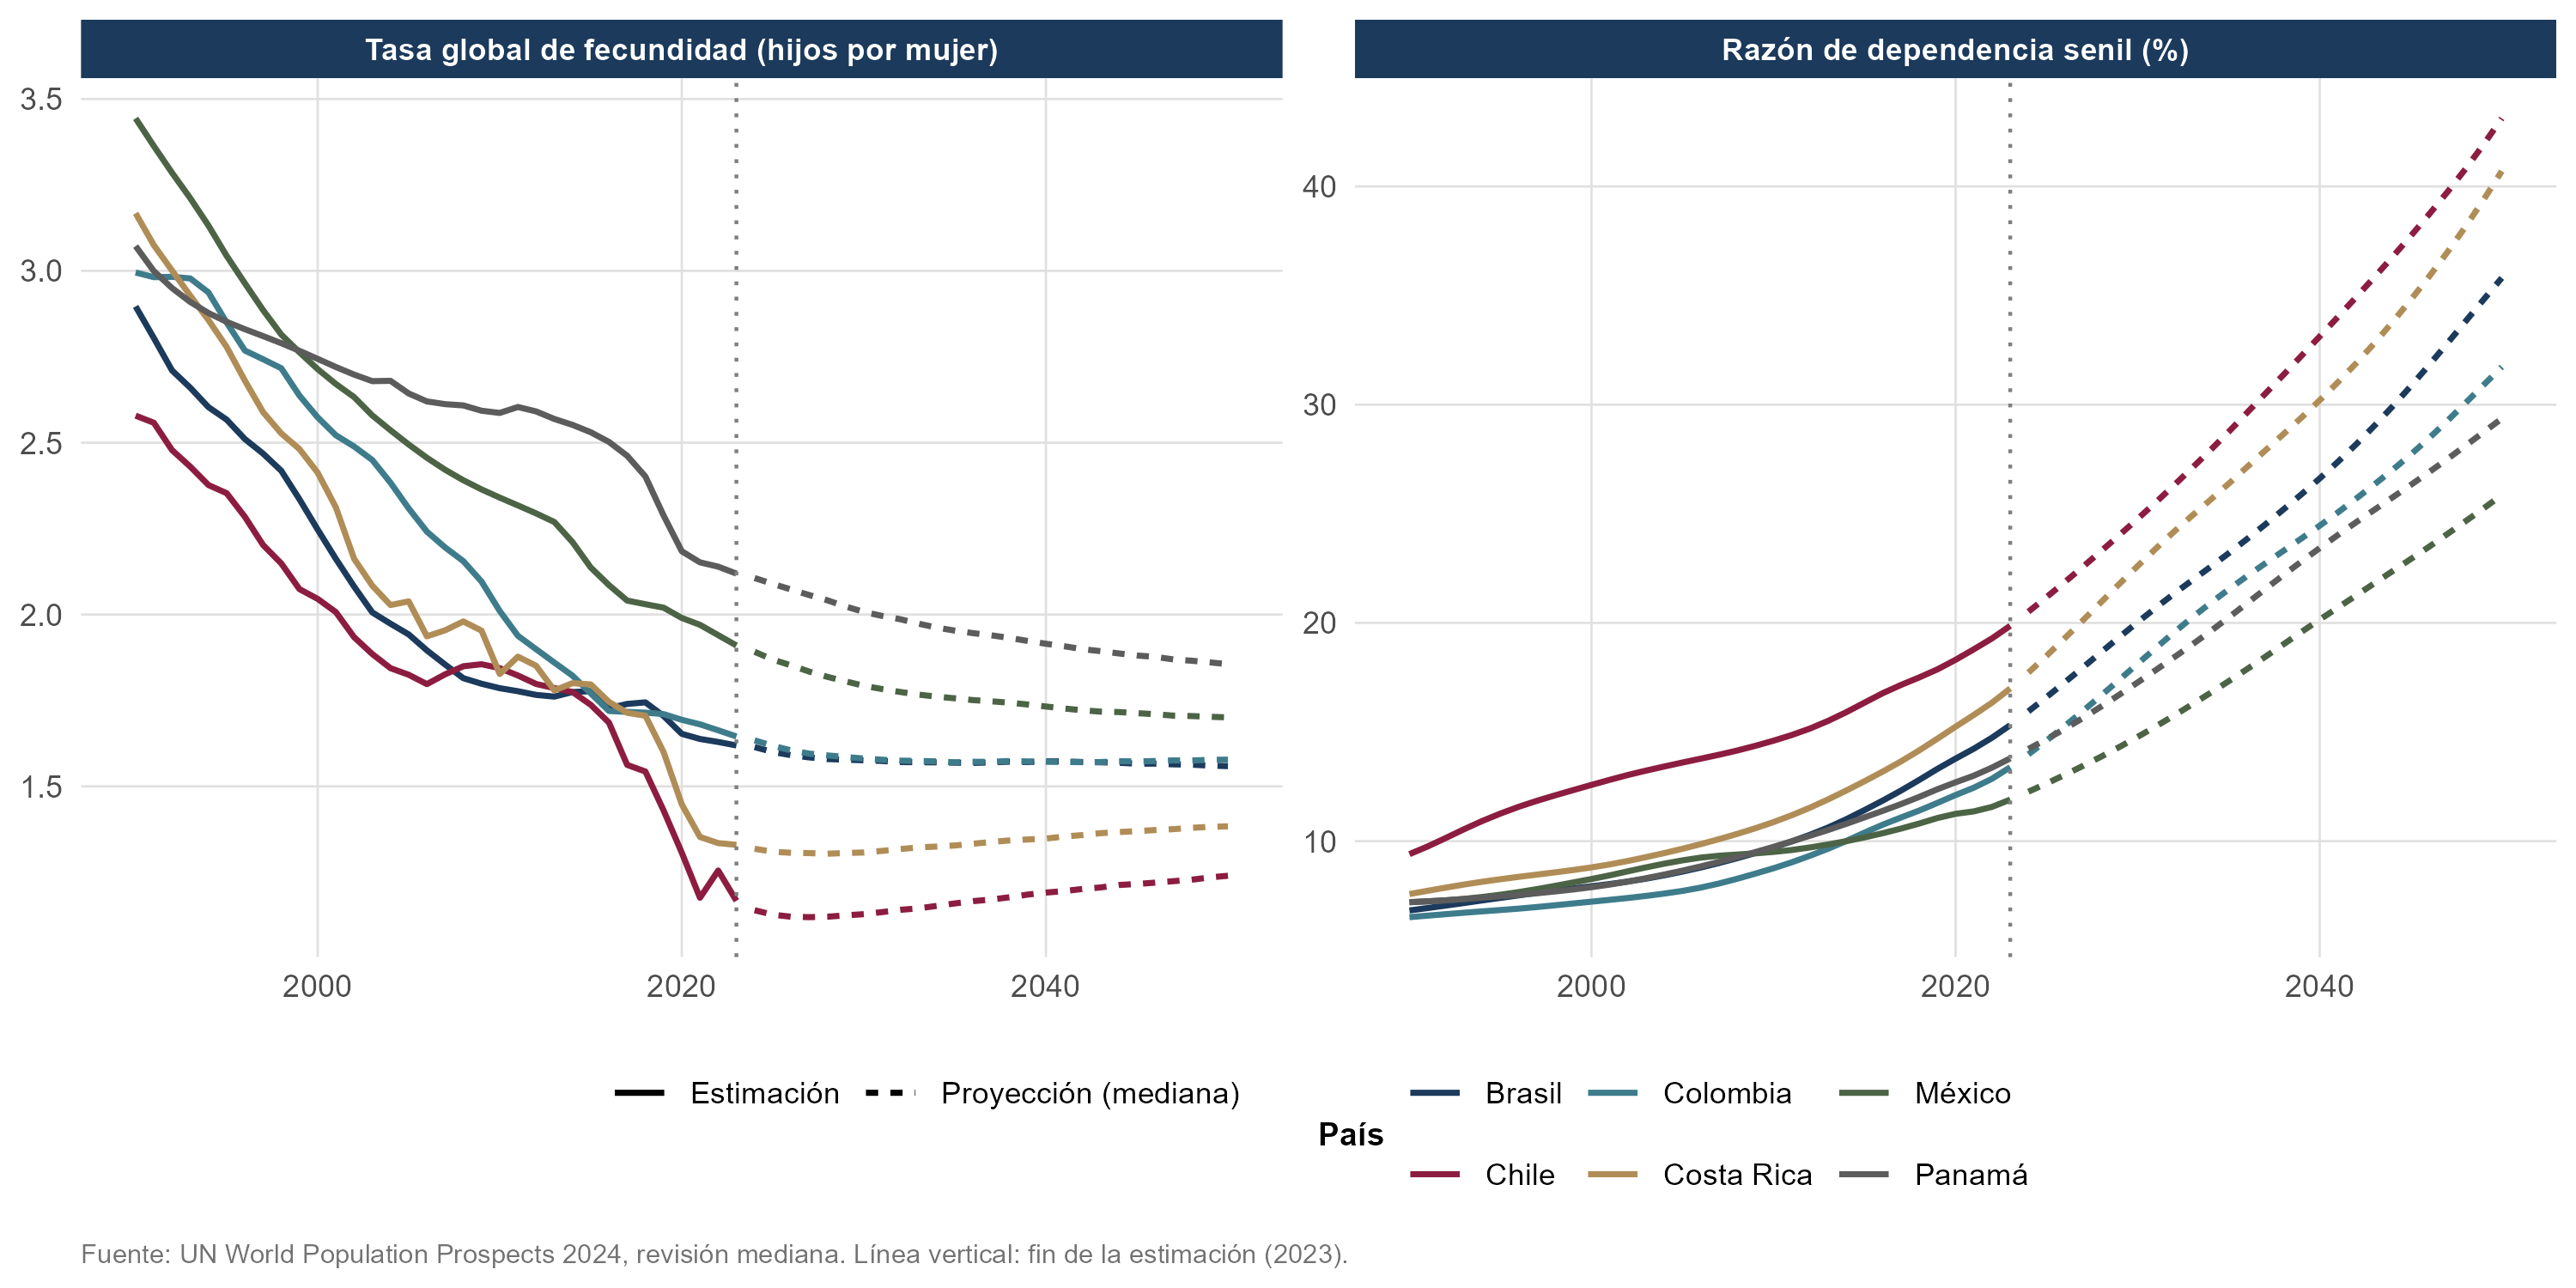
\includegraphics[width=\textwidth]{graficas/fig_demografia.png}
  \caption{Tasa global de fecundidad y razón de dependencia senil, seis países,
  1990--2050. Trazo continuo: estimación (hasta 2023). Trazo discontinuo: proyección
  de la variante mediana. Fuente: UN World Population Prospects 2024.}
  \label{fig:demografia}
\end{figure}

La Tabla~\ref{tab:demog} ya cuantificó el resultado: entre 2025 y 2050 los seis países
multiplican su razón de dependencia senil por un factor de 2,0 a 2,2, con trayectoria
estrictamente ascendente año a año. Conviene subrayar aquí una implicación que la
tabla no hace evidente por sí sola. La dependencia juvenil sigue trayectorias
decrecientes en los seis casos. El tramo final del
bono demográfico es el período en que la relación entre población en edad de trabajar y población dependiente alcanza su punto más favorable, y por tanto el período de mayor
capacidad relativa para generar ingresos tributarios, acumular reservas previsionales o reducir deuda pública. La sección fiscal que sigue evalúa en qué medida los seis países están utilizando esa ventana.

% ---------------------------------------------------------------------
\subsection{Posición fiscal: análisis descriptivo}
\label{sec:posicion-fiscal}
% ---------------------------------------------------------------------

El análisis fiscal se organiza en torno a cinco indicadores, todos expresados como
porcentaje del PIB. Tres describen la posición fiscal agregada —ingresos del gobierno, balance primario y deuda neta del gobierno— y provienen del
\textbf{Fondo Monetario Internacional, World Economic Outlook 2025}, con cobertura 2000--2024. Dos describen el gasto en las funciones directamente expuestas al envejecimiento —salud y pensiones— y provienen de la base de
\textbf{gasto público por función de CEPAL/FMI-GFS}, con cobertura de gobierno central
y disponibilidad que termina entre 2017 y 2020 según el país.

Se emplea deuda neta y no bruta porque descuenta los activos financieros del sector
público, entre ellos las reservas de los regímenes previsionales de capitalización
colectiva, cuya magnitud difiere sustancialmente entre los seis países y
distorsionaría la comparación de posición fiscal si se ignorara. La contrapartida
es que la deuda neta es menos comparable internacionalmente que la bruta, por la
heterogeneidad en la valuación de activos.

Los tres agregados del WEO forman un sistema contable articulado y por eso se presentan
juntos: los ingresos miden la capacidad de recaudación; el balance primario, el resultado de la gestión corriente antes del servicio de la deuda; y la deuda neta, el
resultado acumulado de esa gestión más el efecto de las condiciones financieras. Un balance primario deficitario sostenido se traduce en acumulación de deuda neta, y ésta
determina el margen disponible para absorber presiones futuras de gasto. La
incorporación de la deuda neta es la que permite conectar la fotografía de corto plazo
con la restricción intertemporal que la demografía impone.

Dos advertencias de medición condicionan la lectura y se mantienen vigentes en todo el
análisis posterior. Primera: en el WEO los valores de 2024 son estimación del FMI en
Brasil, Costa Rica y Panamá, y dato observado en Chile, Colombia y México. Segunda, más relevante: el gasto funcional tiene cobertura de \emph{gobierno central}. En los
países donde salud y pensiones se financian principalmente a través de instituciones de
seguridad social con autonomía presupuestaria —la CCSS en Costa Rica, la CSS en Panamá,
y de forma parcial IMSS e ISSSTE en México— los niveles registrados subestiman el gasto
público efectivo en esas funciones. Las series son internamente consistentes en el
tiempo, que es la propiedad que el análisis de series de tiempo requiere, pero sus
niveles no son directamente comparables entre países sin esta salvedad.

\subsubsection{Agregados fiscales}
\label{sec:agregados}

Las Figuras~\ref{fig:ingresos} a~\ref{fig:deuda} presentan la evolución de los tres agregados del WEO. La heterogeneidad de niveles es el primer rasgo a destacar: Brasil recauda de forma sostenida entre 35 y 40\,\% del PIB, mientras Costa Rica y Panamá se
sitúan en el rango de 13 a 17\,\%. Esta diferencia de más de veinte puntos porcentuales
del PIB en capacidad de recaudación es determinante de la capacidad de absorción del choque demográfico, y refuerza el punto planteado en la
Sección~\ref{sec:envejecer-antes} sobre el envejecimiento con bases tributarias estrechas.

\begin{figure}[htbp]
  \centering
  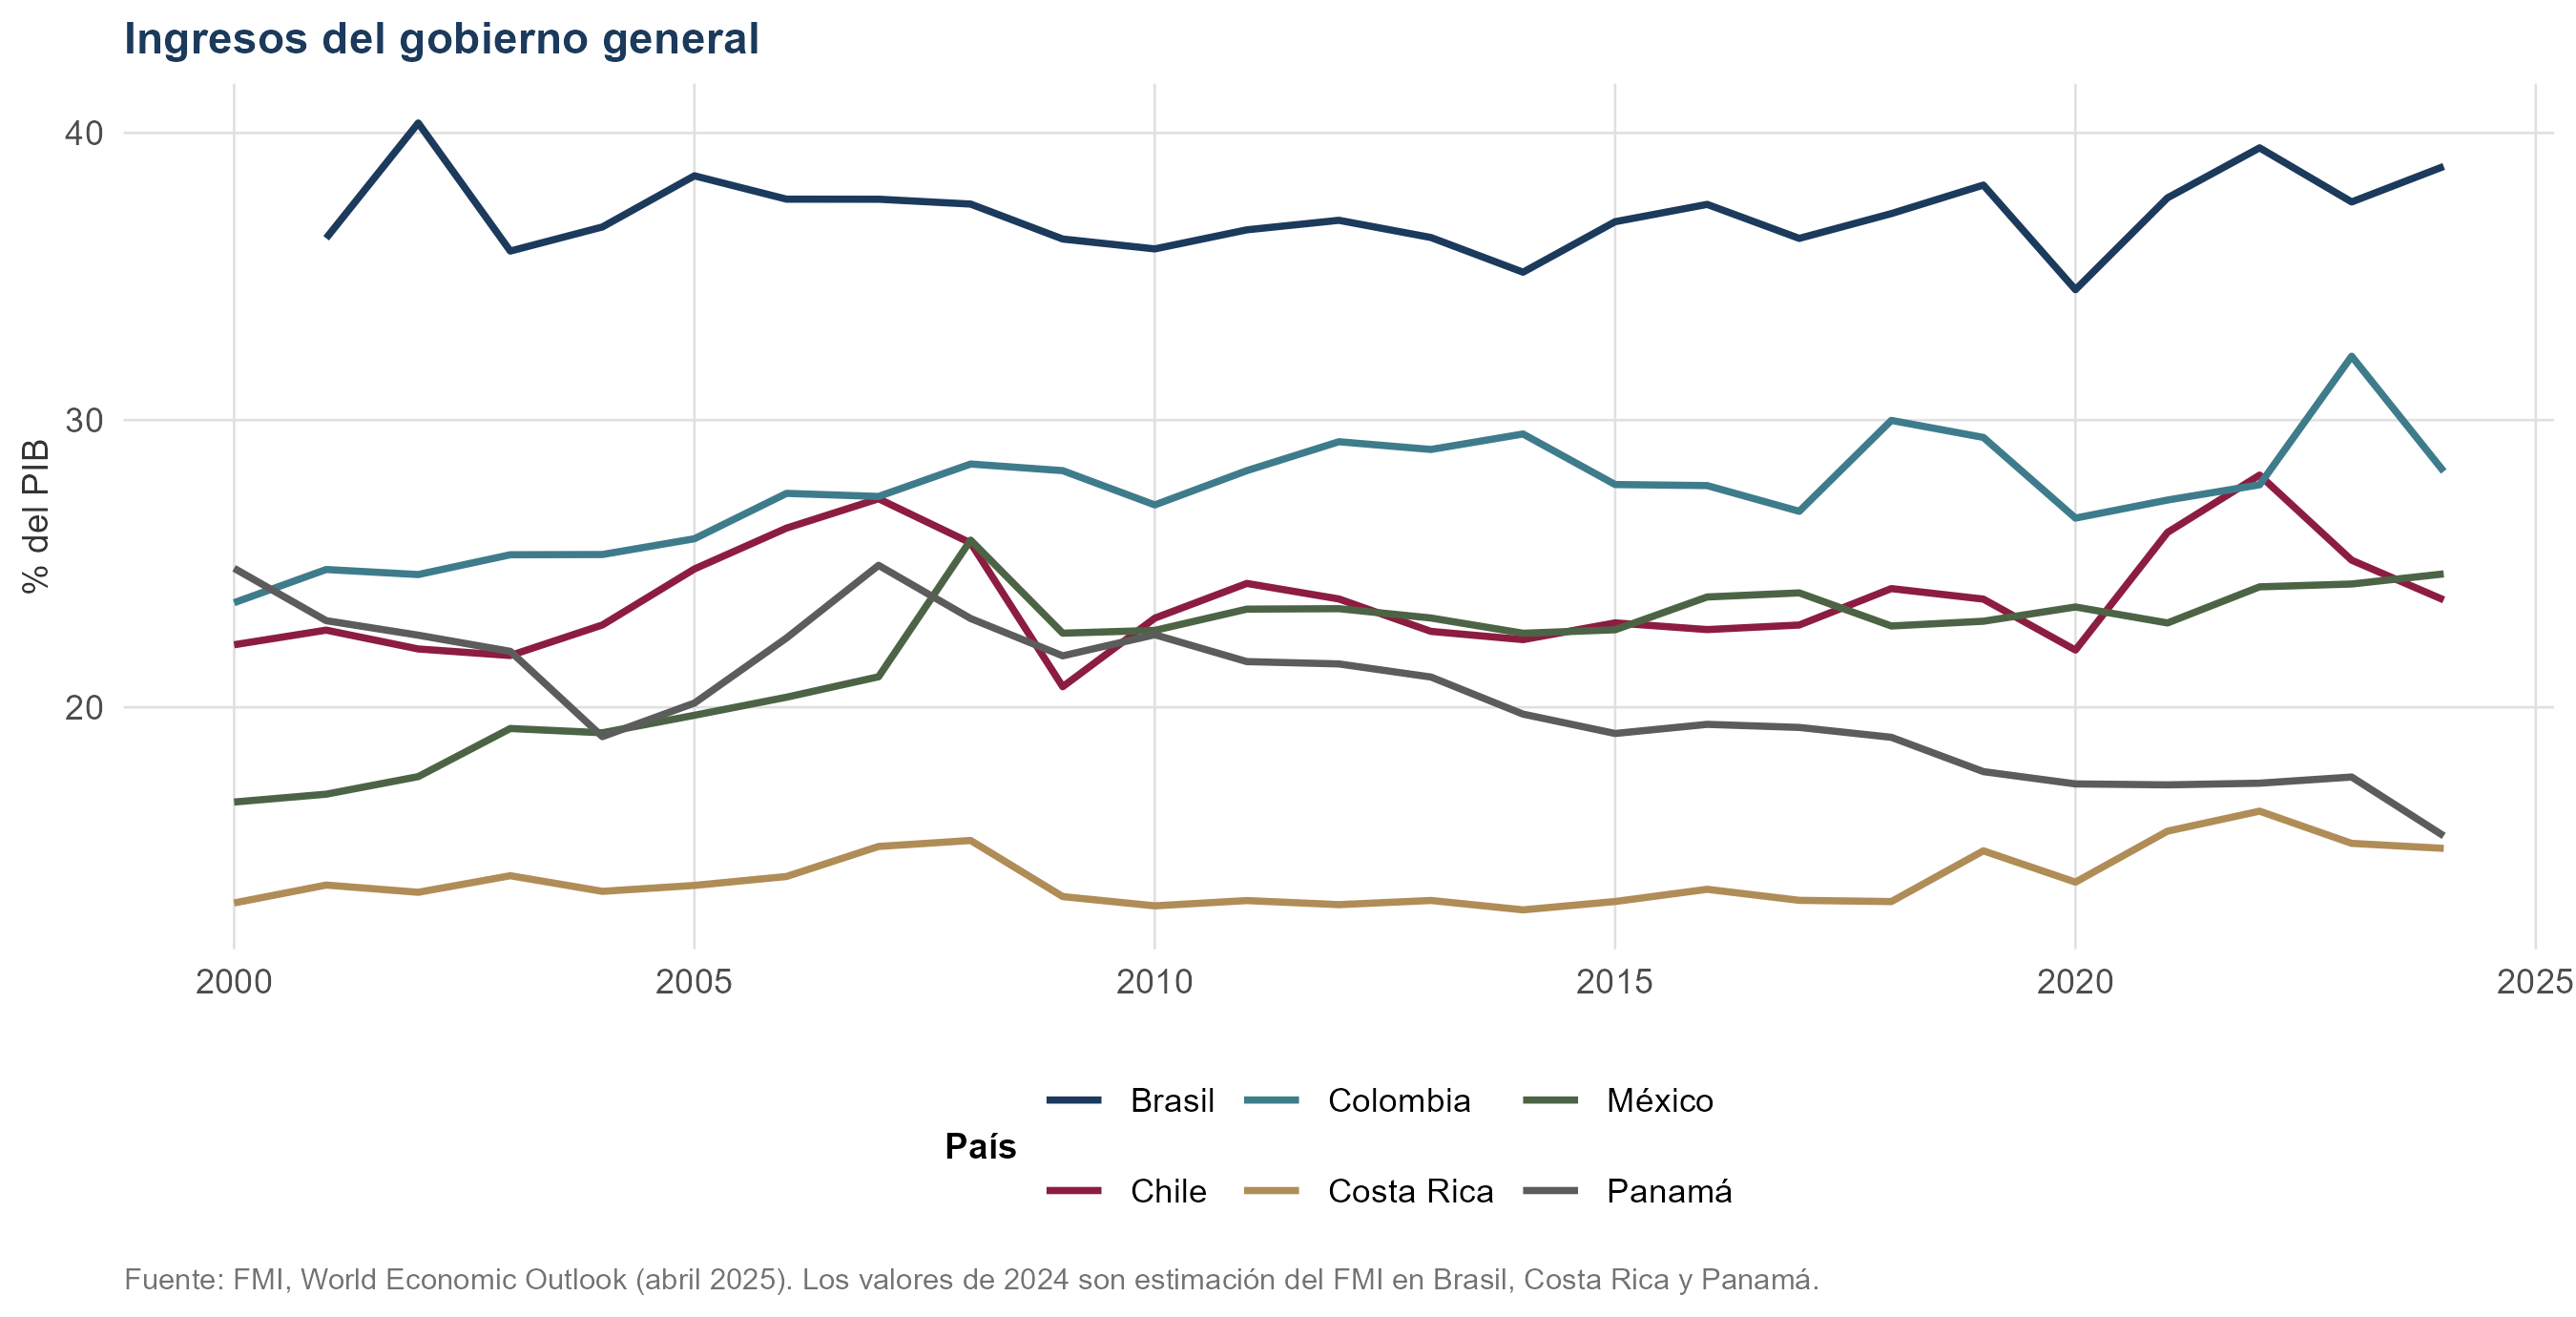
\includegraphics[width=0.92\textwidth]{graficas/fig_ingresos.png}
  \caption{Ingresos del gobierno general (\% del PIB), 2000--2024.
  Fuente: FMI, World Economic Outlook, abril de 2025.}
  \label{fig:ingresos}
\end{figure}

\begin{figure}[htbp]
  \centering
  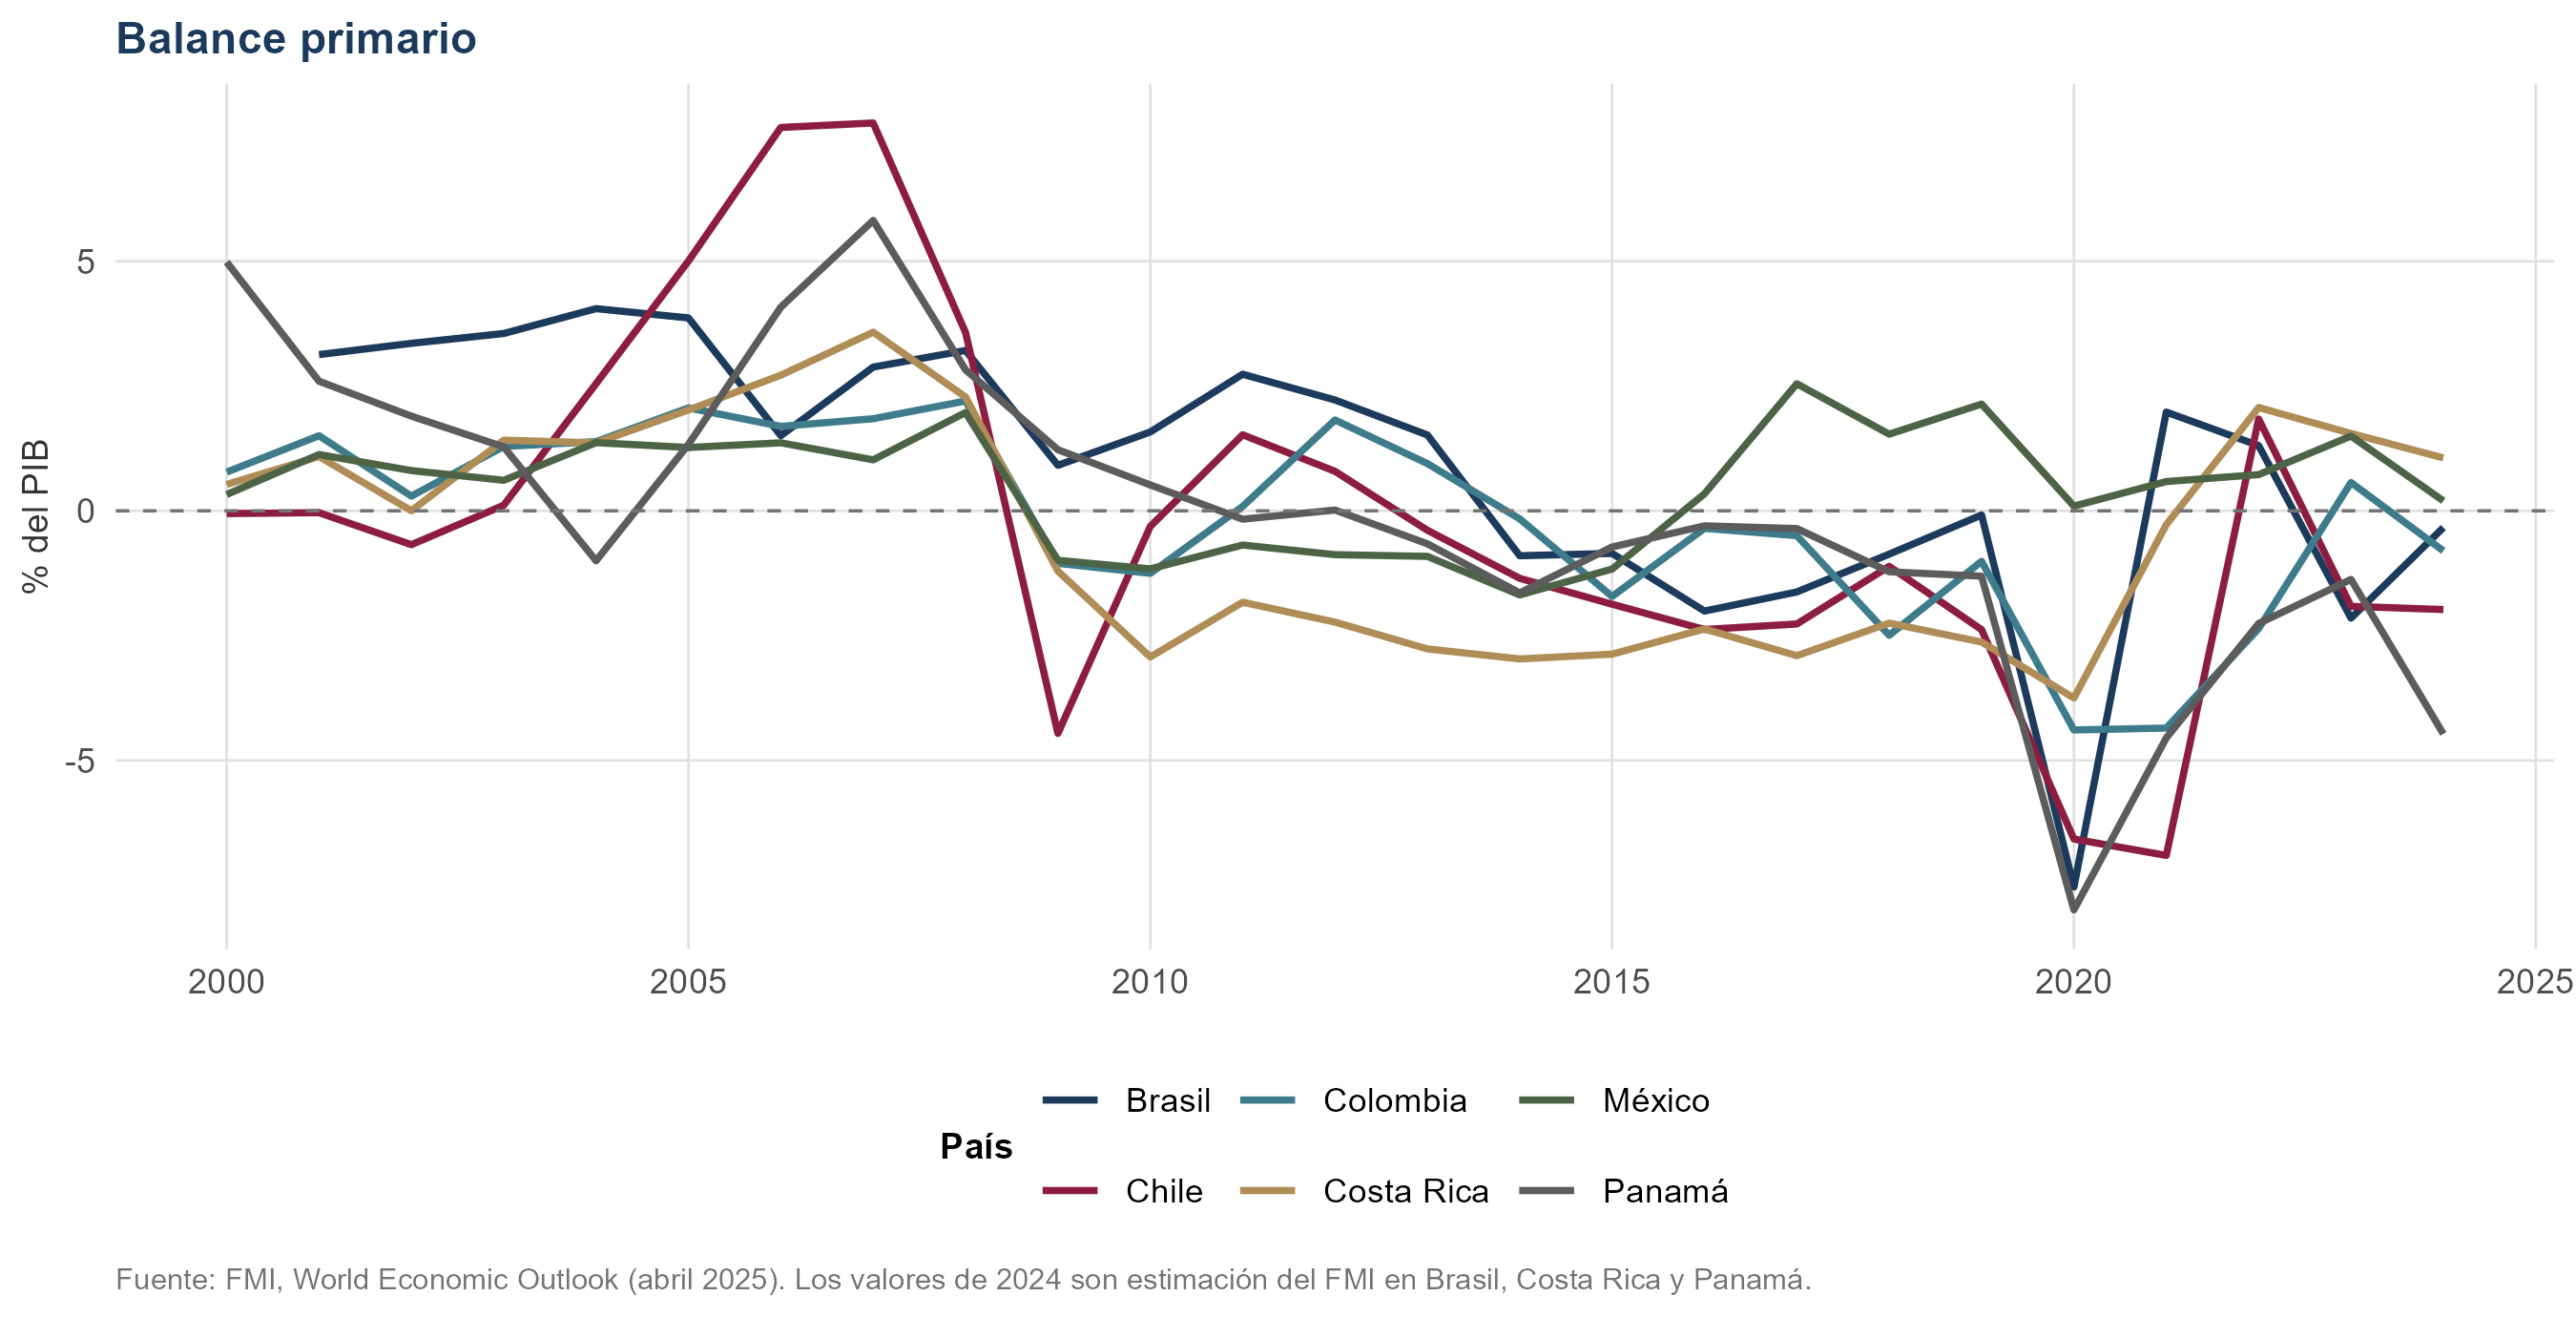
\includegraphics[width=0.92\textwidth]{graficas/fig_balance.png}
  \caption{Balance primario del gobierno general (\% del PIB), 2000--2024.
  Fuente: FMI, World Economic Outlook, abril de 2025.}
  \label{fig:balance}
\end{figure}

\begin{figure}[htbp]
  \centering
  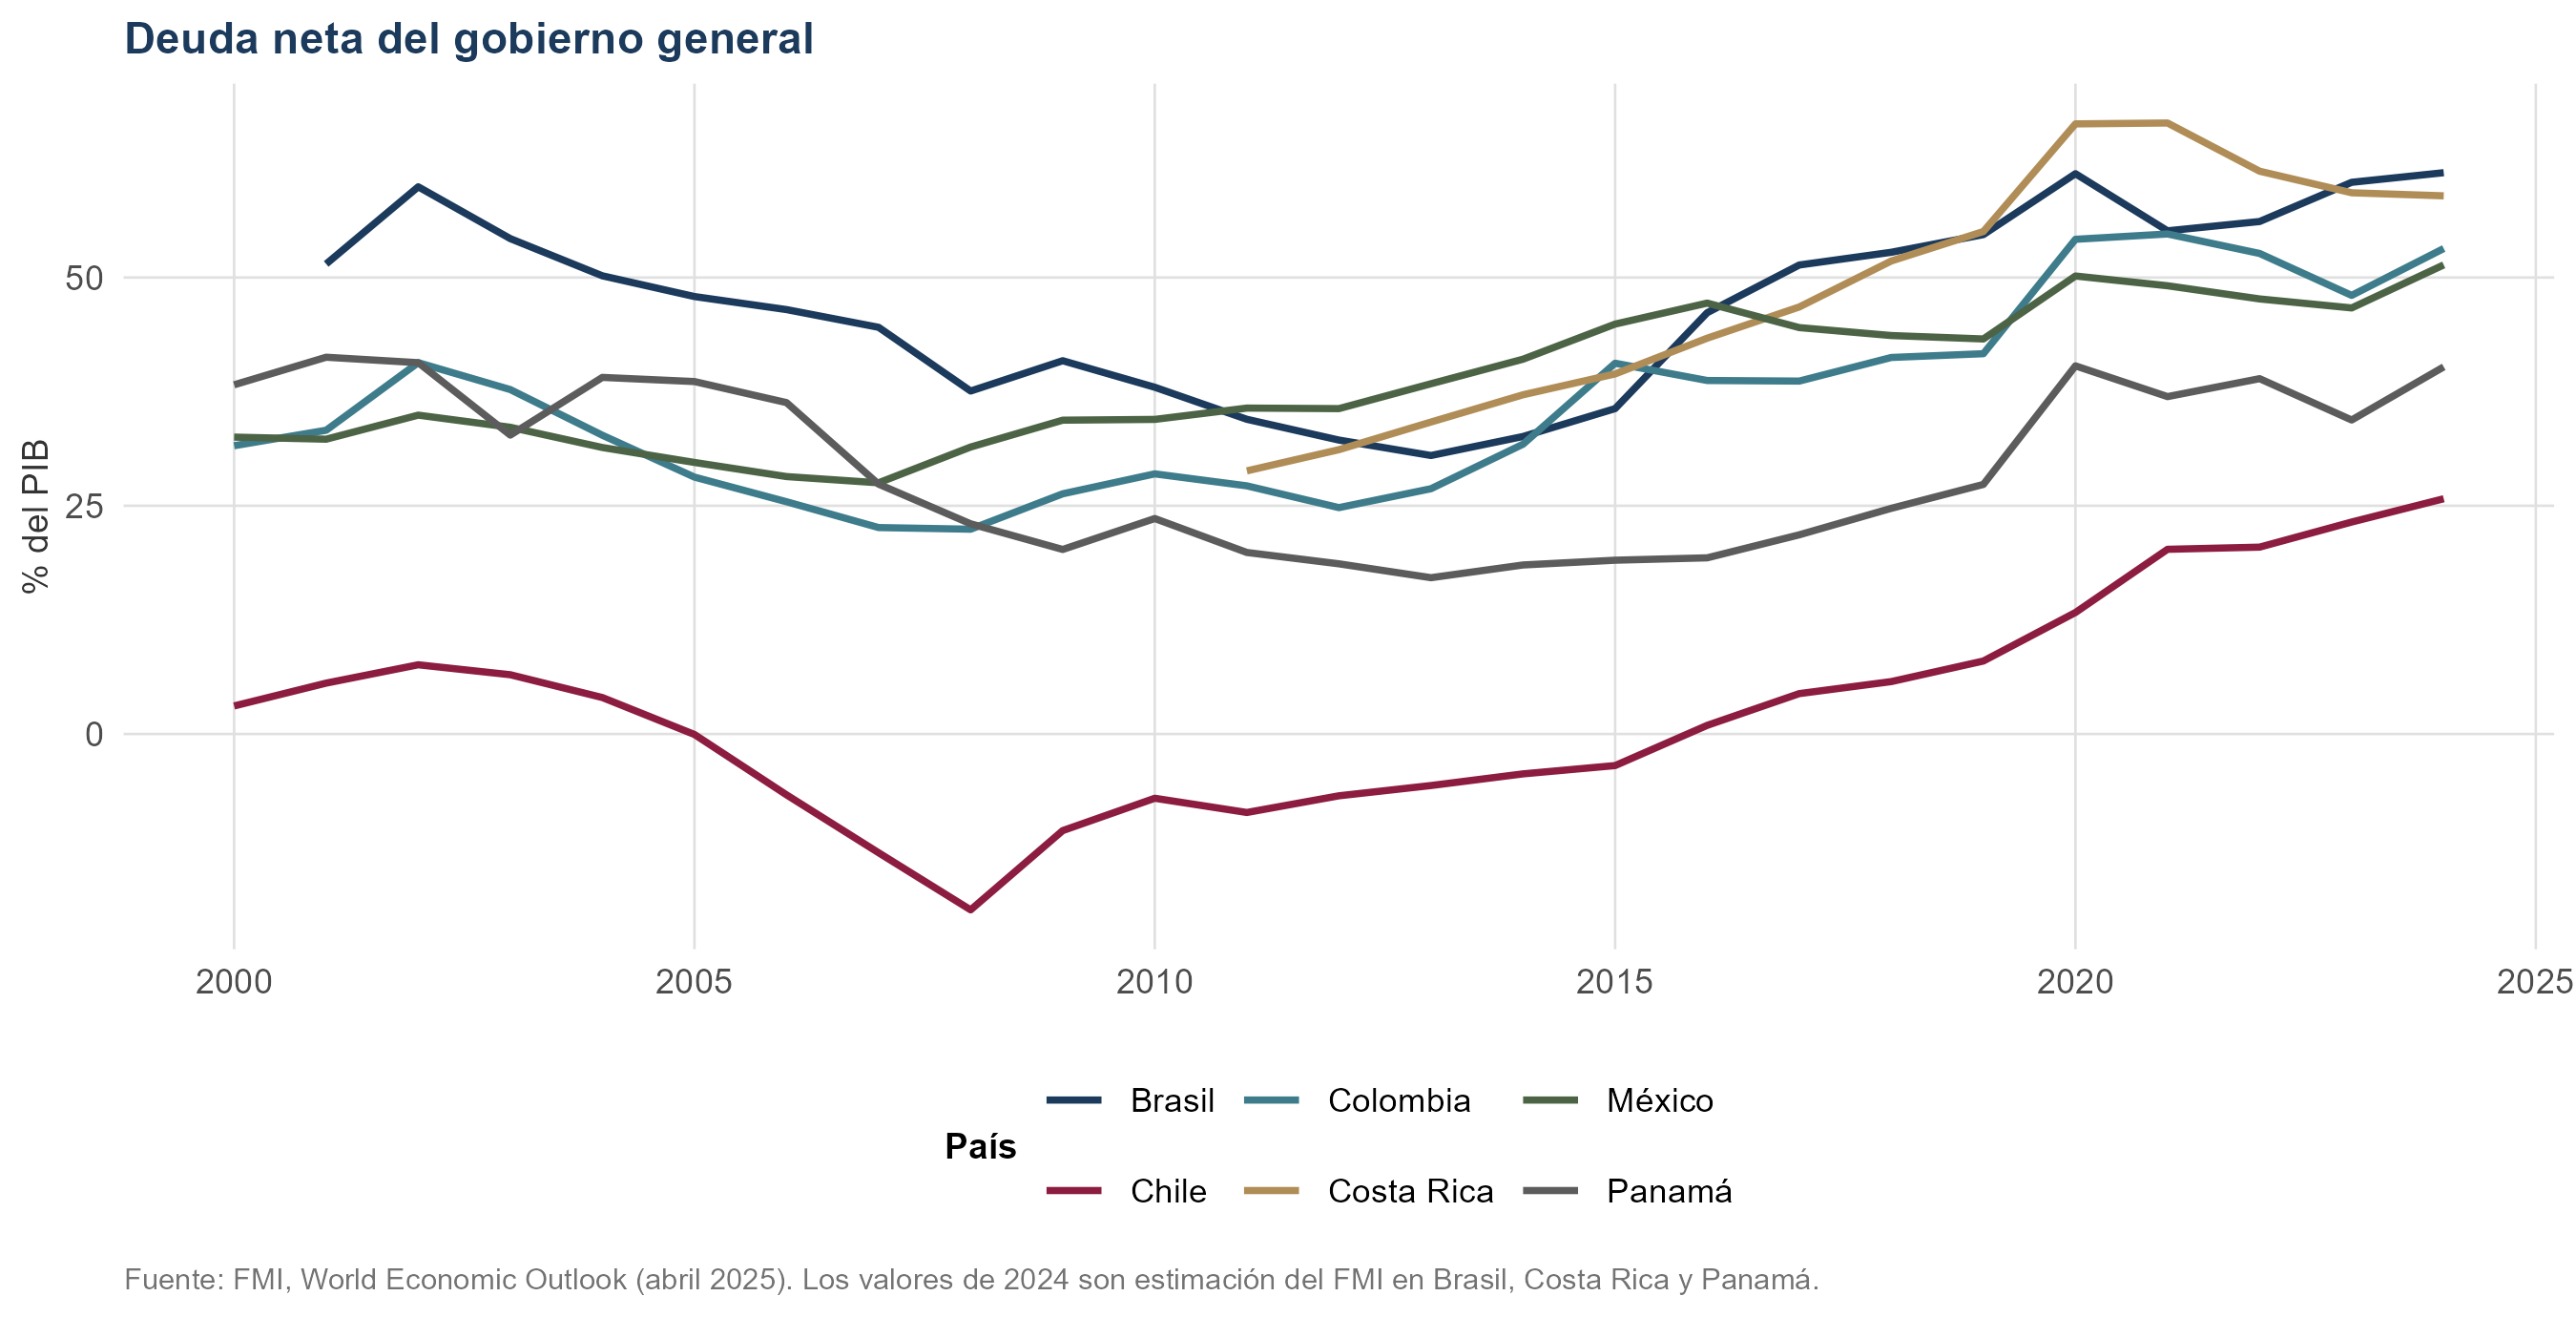
\includegraphics[width=0.92\textwidth]{graficas/fig_deuda.png}
  \caption{Deuda neta del gobierno general (\% del PIB), 2000--2024.
  Fuente: FMI, World Economic Outlook, abril de 2025.}
  \label{fig:deuda}
\end{figure}

El balance primario muestra el comportamiento procíclico esperable: mínimos históricos en 2020--2021 asociados al choque sanitario. La recuperación
posterior ha sido parcial y desigual. La deuda neta, en cambio, exhibe una trayectoria
ascendente que no revierte con la misma velocidad: el nivel alcanzado tras la pandemia
se consolida en la mayoría de los casos, y en 2024 supera el 50\,\% del PIB en cuatro de
los seis países.

La Tabla~\ref{tab:ultimo-weo} sintetiza la posición en el último año disponible. La variación se reporta como \emph{diferencia en puntos porcentuales} respecto al año previo: al estar las series ya expresadas en porcentaje del PIB, el cambio en puntos porcentuales es la métrica interpretable.

\begin{table}[htbp]
  \centering
  \caption{Agregados fiscales en 2024 y variación respecto a 2023
  (\% del PIB; variación en puntos porcentuales).}
  \label{tab:ultimo-weo}
  \begin{tabular}{lcccccc}
    \toprule
    & \multicolumn{2}{c}{Ingresos} & \multicolumn{2}{c}{Balance primario}
    & \multicolumn{2}{c}{Deuda neta} \\
    \cmidrule(lr){2-3}\cmidrule(lr){4-5}\cmidrule(lr){6-7}
    País & 2024 & $\Delta$ & 2024 & $\Delta$ & 2024 & $\Delta$ \\
    \midrule
    Brasil     & 38.8 & $+1.2$ & $-0.3$ & $+1.8$ & 61.5 & $+1.1$ \\
    Chile      & 23.7 & $-1.4$ & $-2.0$ & $-0.1$ & 25.8 & $+2.6$ \\
    Colombia   & 28.2 & $-4.0$ & $-0.8$ & $-1.4$ & 53.2 & $+5.1$ \\
    Costa Rica & 15.1 & $-0.2$ & $+1.1$ & $-0.5$ & 58.9 & $-0.3$ \\
    México     & 24.6 & $+0.4$ & $+0.2$ & $-1.3$ & 51.4 & $+4.7$ \\
    Panamá     & 15.5 & $-2.0$ & $-4.5$ & $-3.1$ & 40.2 & $+5.8$ \\
    \bottomrule
  \end{tabular}

  \vspace{2pt}
  \footnotesize
  Fuente: FMI, World Economic Outlook, abril de 2025. Los valores de 2024 son
  estimación del FMI en Brasil, Costa Rica y Panamá, y observados en Chile, Colombia
  y México.
\end{table}

El patrón de 2024 merece atención. Cinco de los seis países registran deterioro del
balance primario respecto a 2023, y cinco de seis aumentan su deuda neta. Los casos de
Panamá y Colombia son los más pronunciados: Panamá combina una caída de ingresos de 2,0 puntos con un deterioro del balance primario de 3,1 puntos y un aumento de deuda neta de 5,8 puntos en un solo ejercicio; Colombia registra la mayor contracción de
ingresos de la muestra (4,0 puntos) junto con un aumento de deuda de 5,1 puntos. Este deterioro ocurre en la fase en que la dependencia senil todavía se encuentra en niveles bajos respecto a su trayectoria proyectada, lo que significa que el punto de partida
fiscal se está debilitando precisamente durante la ventana en que sería más favorable fortalecerlo.

\subsubsection{Gasto en salud y pensiones}
\label{sec:gfs-funcional}

Antes de leer estas series conviene reconciliarlas con las de la
Sección~\ref{sec:esquemas-salud}. Los niveles de gasto público en salud que aquí se
reportan son sistemáticamente inferiores a los de la Tabla~\ref{tab:salud} porque
miden cosas distintas: la Tabla~\ref{tab:salud} recoge el gasto público total en
salud según la clasificación GHED de la Organización Mundial de la Salud, que
incorpora los esquemas de seguro social obligatorio con independencia de su
ubicación institucional; las series de esta sección proceden de la base de gasto
por función de CEPAL/FMI-GFS con \textbf{cobertura de gobierno central}, que
excluye a las instituciones de seguridad social con autonomía presupuestaria. La
brecha es mayor donde esa autonomía es mayor: Costa Rica registra 4,61\,\% del PIB
en la Tabla~\ref{tab:salud} y 0,69\,\% en la Tabla~\ref{tab:ultimo-gfs}, diferencia
que corresponde casi enteramente al Seguro de Enfermedad y Maternidad de la CCSS;
Panamá presenta la misma discrepancia por la CSS, y México una versión atenuada por
el IMSS y el ISSSTE. \textbf{Los niveles de esta sección no deben citarse como
medida del gasto público en salud de estos países; su utilidad es la consistencia
interna en el tiempo, que es la propiedad que requiere el análisis de series que
sigue.}

Las Figuras~\ref{fig:salud} y~\ref{fig:pensiones} presentan el gasto en las dos
funciones directamente expuestas al envejecimiento. La tendencia es creciente en la
mayoría de los países, con dos casos destacados: Chile, cuyo gasto público en salud
pasa de 1,8 a 6,0\,\% del PIB entre 1990 y 2020, y México, cuyo gasto en pensiones
crece hasta 3,0\,\% del PIB en 2020,
reflejo de la maduración del régimen de transición documentado en la Sección~\ref{sec:mexico}. Brasil presenta el nivel más alto de la muestra en pensiones (8,8\,\% del
PIB), consistente con un sistema de reparto de cobertura amplia y beneficio definido.

\begin{figure}[htbp]
  \centering
  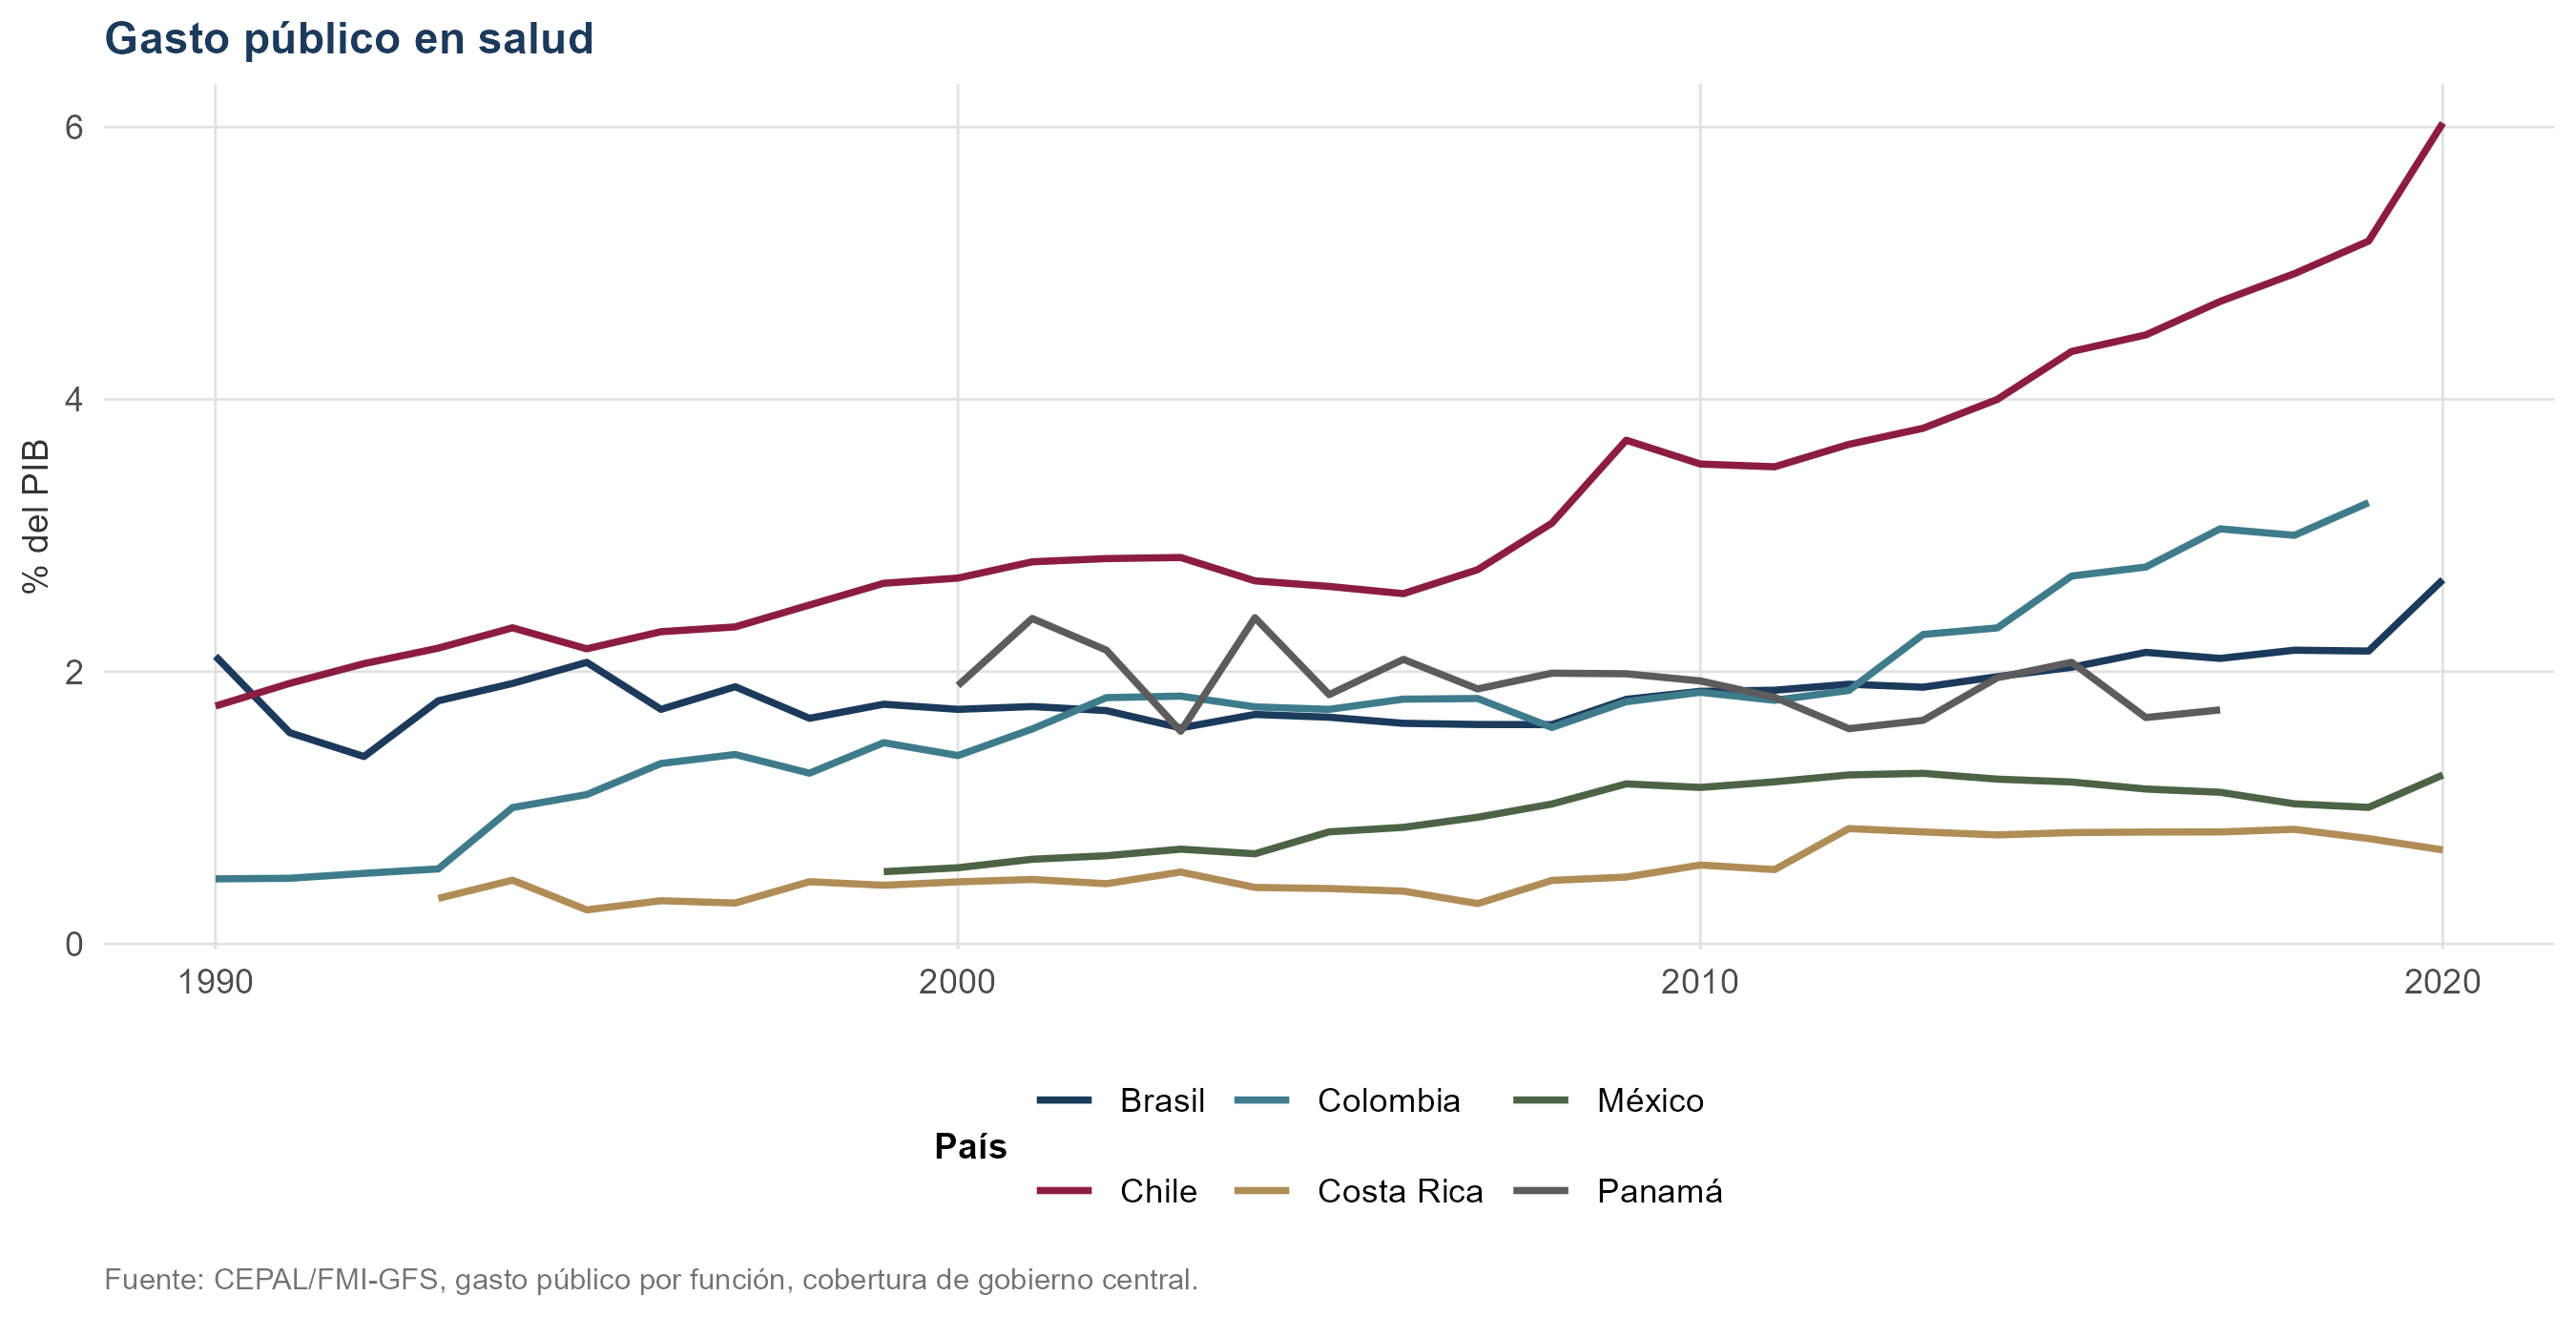
\includegraphics[width=0.92\textwidth]{graficas/fig_salud.png}
  \caption{Gasto público en salud (\% del PIB), gobierno central.
  Fuente: CEPAL/FMI-GFS, gasto público por función.}
  \label{fig:salud}
\end{figure}

\begin{figure}[htbp]
  \centering
  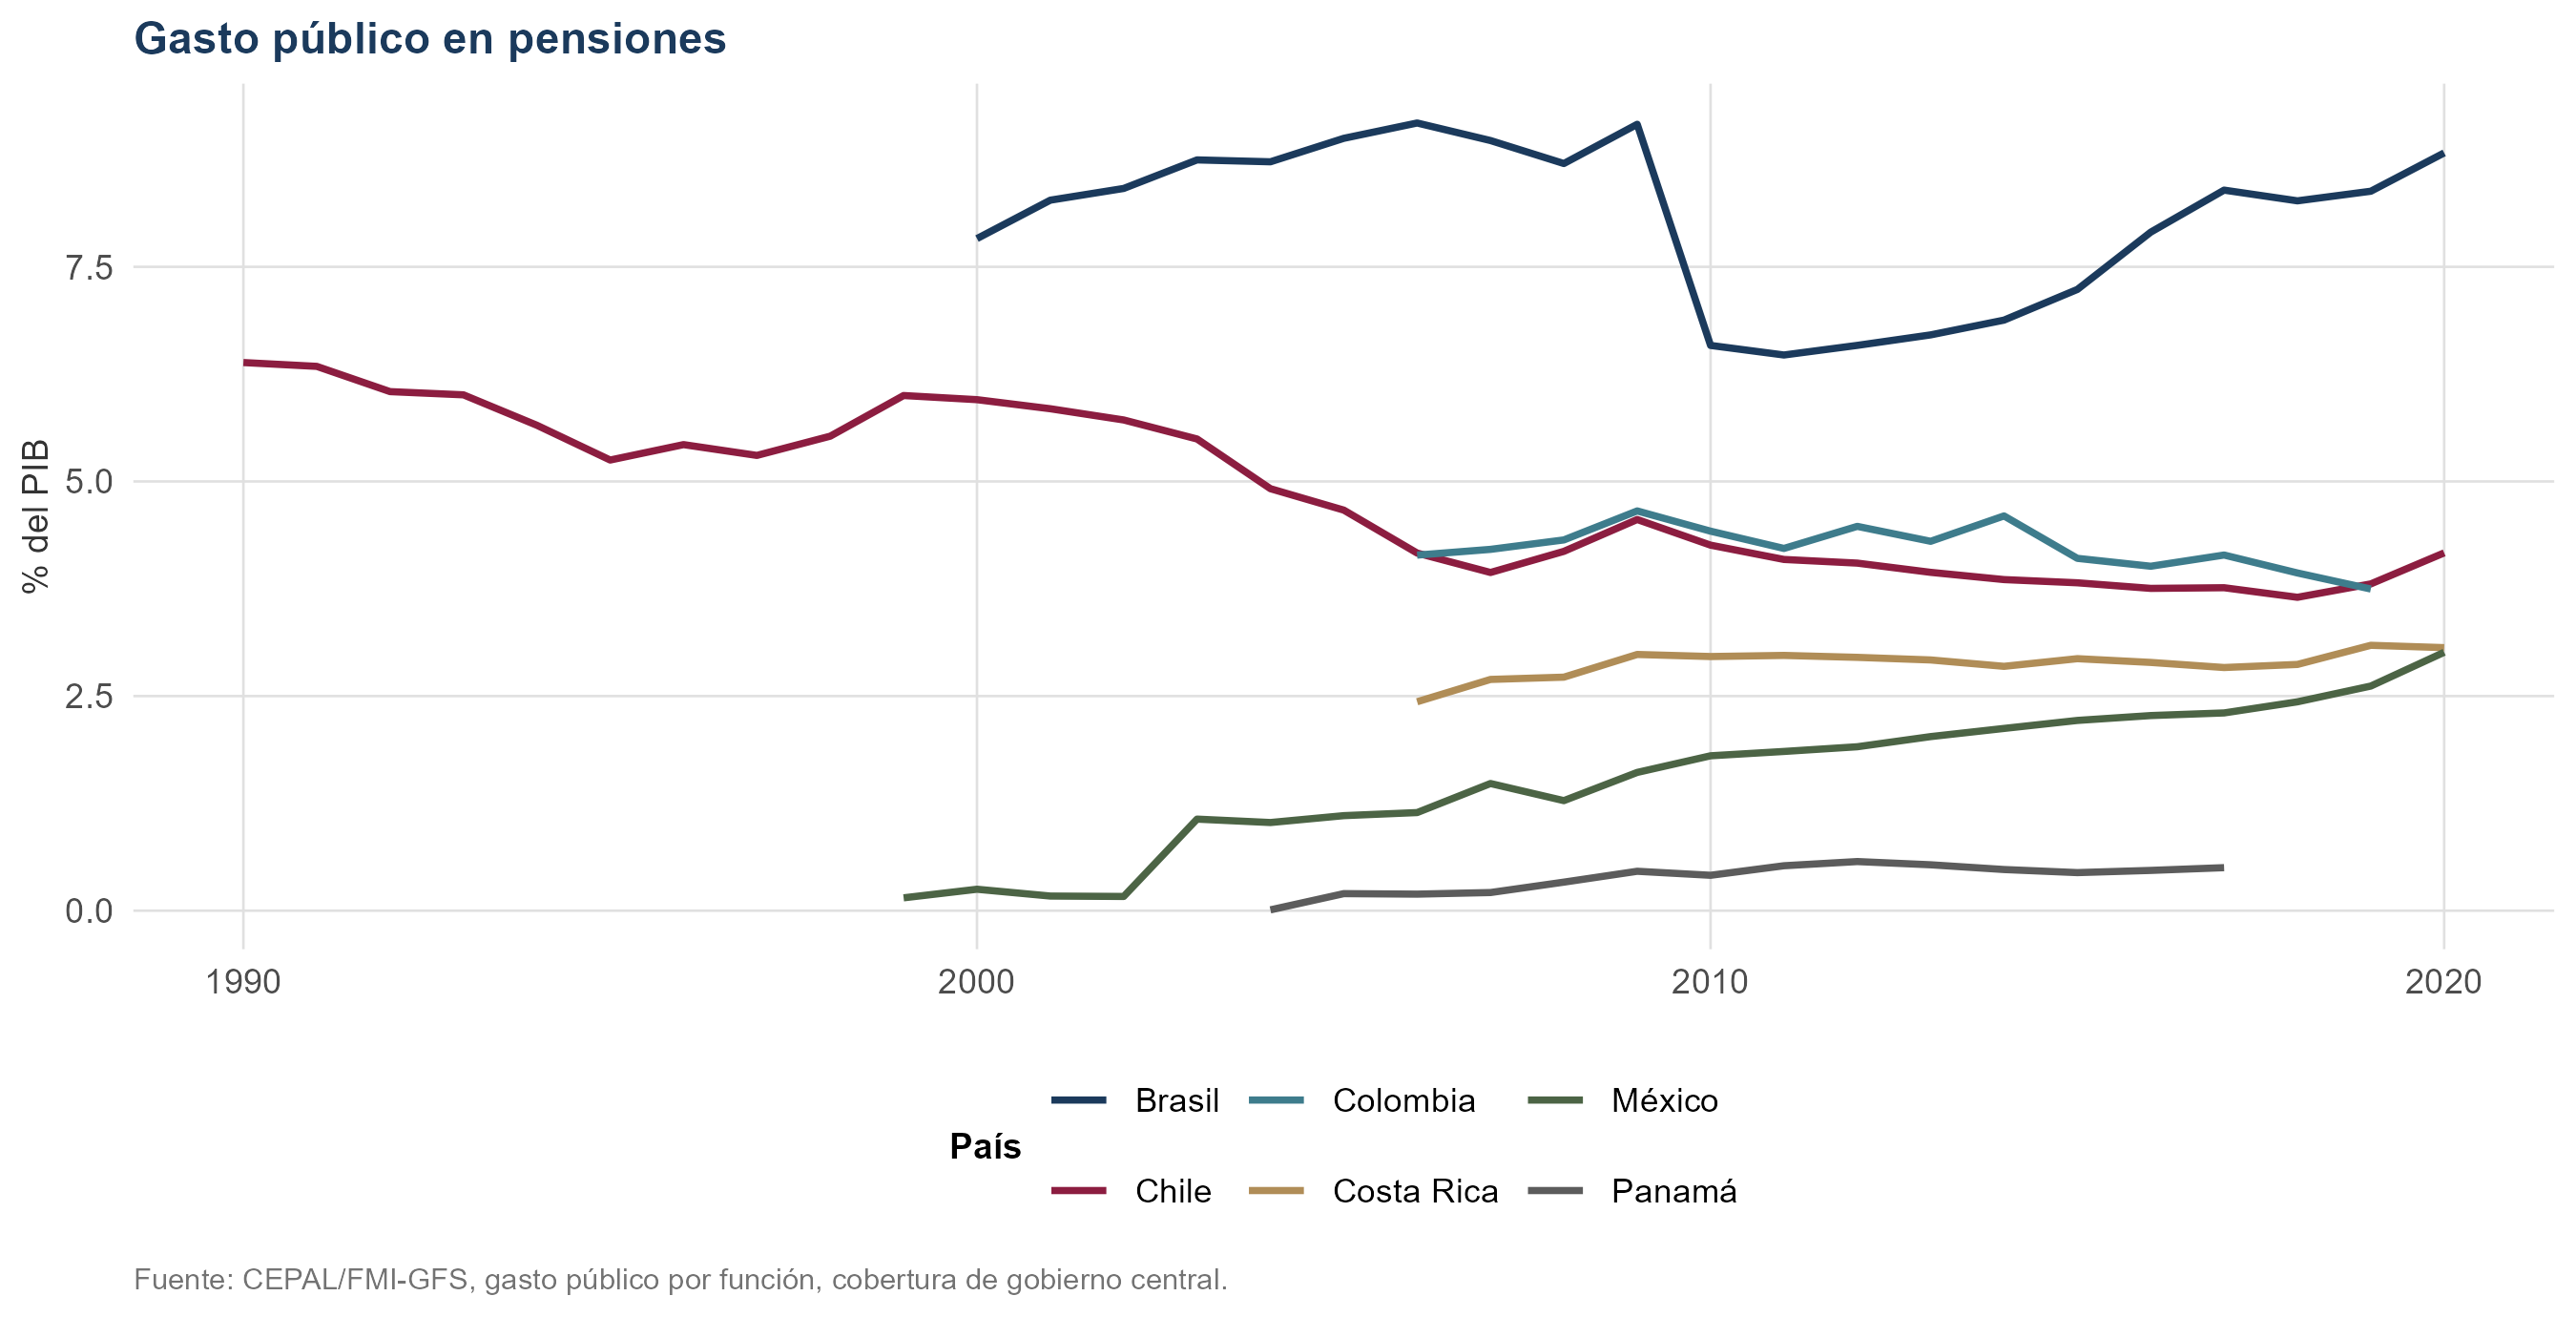
\includegraphics[width=0.92\textwidth]{graficas/fig_pensiones.png}
  \caption{Gasto público en pensiones (\% del PIB), gobierno central.
  Serie construida como suma de las funciones \emph{edad avanzada} y
  \emph{enfermedad e incapacidad} donde la cobertura de la segunda lo permite;
  en caso contrario, sólo \emph{edad avanzada}.
  Fuente: CEPAL/FMI-GFS, gasto público por función.}
  \label{fig:pensiones}
\end{figure}

La Tabla~\ref{tab:ultimo-gfs} reporta el último dato disponible y su variación. A diferencia de los agregados del WEO, aquí el año de corte difiere entre países, y en cuatro de los seis casos corresponde a 2020. Esto implica que la variación reportada captura el choque sanitario y no una tendencia estructural: los incrementos de salud en
Brasil (0,52 puntos) y Chile (0,87 puntos) reflejan la respuesta fiscal a la pandemia, no un cambio de régimen de gasto. La interpretación estructural de estas series debe
apoyarse en la trayectoria completa de las Figuras~\ref{fig:salud} y~\ref{fig:pensiones}, no en la última variación anual.

\begin{table}[htbp]
  \centering
  \caption{Gasto en salud y pensiones: último año disponible y variación respecto al
  año previo (\% del PIB; variación en puntos porcentuales).}
  \label{tab:ultimo-gfs}
  \begin{tabular}{lccccc}
    \toprule
    & & \multicolumn{2}{c}{Salud} & \multicolumn{2}{c}{Pensiones} \\
    \cmidrule(lr){3-4}\cmidrule(lr){5-6}
    País & Año & Nivel & $\Delta$ & Nivel & $\Delta$ \\
    \midrule
    Brasil     & 2020 & 2.67 & $+0.52$ & 8.83 & $+0.45$ \\
    Chile      & 2020 & 6.03 & $+0.87$ & 4.17 & $+0.36$ \\
    Colombia   & 2019 & 3.24 & $+0.24$ & 3.75 & $-0.19$ \\
    Costa Rica & 2020 & 0.69 & $-0.08$ & 3.06 & $-0.03$ \\
    México     & 2020 & 1.24 & $+0.24$ & 3.01 & $+0.39$ \\
    Panamá     & 2017 & 1.72 & $+0.06$ & 0.50 & $+0.03$ \\
    \bottomrule
  \end{tabular}

  \vspace{2pt}
  \footnotesize
  Fuente: CEPAL/FMI-GFS, gasto público por función, cobertura de gobierno central.
  Los niveles de Costa Rica y Panamá subestiman el gasto público efectivo por operar
  su seguridad social (CCSS y CSS) fuera del perímetro del gobierno central. En cuatro
  de los seis países el último año disponible es 2020, por lo que la variación captura
  el efecto de la pandemia. Los niveles no son comparables con los de la
  Tabla~\ref{tab:salud} (GHED, cobertura institucional completa); véase la
  reconciliación al inicio de esta subsección.
\end{table}

\subsubsection{Importancia relativa de pensiones y salud en el gasto público}
\label{sec:composicion}

La expresión del gasto como porcentaje del PIB mide la carga sobre la economía, pero no informa sobre su peso dentro del presupuesto. Esa segunda dimensión es la que determina el grado de rigidez presupuestaria: cuanto mayor sea la fracción del gasto público
comprometida en funciones cuya demanda está determinada demográficamente, menor es el margen de reasignación disponible ante un choque. La Tabla~\ref{tab:composicion} y la
Figura~\ref{fig:composicion} presentan la participación de salud y pensiones en el gasto
público total.

\begin{table}[htbp]
  \centering
  \caption{Participación de salud y pensiones en el gasto público total,
  último año con dato simultáneo.}
  \label{tab:composicion}
  \begin{tabular}{lccccccc}
    \toprule
    & & \multicolumn{3}{c}{\% del PIB} & \multicolumn{3}{c}{\% del gasto público} \\
    \cmidrule(lr){3-5}\cmidrule(lr){6-8}
    País & Año & Salud & Pens. & Gasto tot. & Salud & Pens. & Suma \\
    \midrule
    Chile      & 2020 & 6.03 & 4.17 & 29.1 & 20.7 & 14.3 & 35.1 \\
    Brasil     & 2020 & 2.67 & 8.83 & 46.2 & 5.8  & 19.1 & 24.9 \\
    Colombia   & 2019 & 3.24 & 3.75 & 32.9 & 9.9  & 11.4 & 21.3 \\
    Costa Rica & 2020 & 0.69 & 3.06 & 22.3 & 3.1  & 13.7 & 16.8 \\
    México     & 2020 & 1.24 & 3.01 & 27.8 & 4.5  & 10.8 & 15.3 \\
    Panamá     & 2017 & 1.72 & 0.50 & 21.2 & 8.1  & 2.4  & 10.5 \\
    \bottomrule
  \end{tabular}

  \vspace{2pt}
  \footnotesize
  Fuentes: CEPAL/FMI-GFS (gasto funcional, gobierno central) y FMI-WEO
  (gasto total del gobierno general, abril de 2025). Las participaciones combinan
  numerador de gobierno central con denominador de gobierno general, por lo que
  constituyen una \textbf{cota inferior} del peso presupuestario efectivo,
  particularmente en Costa Rica y Panamá, donde la seguridad social opera fuera del
  perímetro del gobierno central. Los valores son comparables en el tiempo dentro de
  cada país, no estrictamente entre países. El numerador de salud no es comparable
  con el gasto público en salud de la Tabla~\ref{tab:salud} (GHED); véase la
  reconciliación al inicio de la Sección~\ref{sec:gfs-funcional}.
\end{table}

\begin{figure}[htbp]
  \centering
  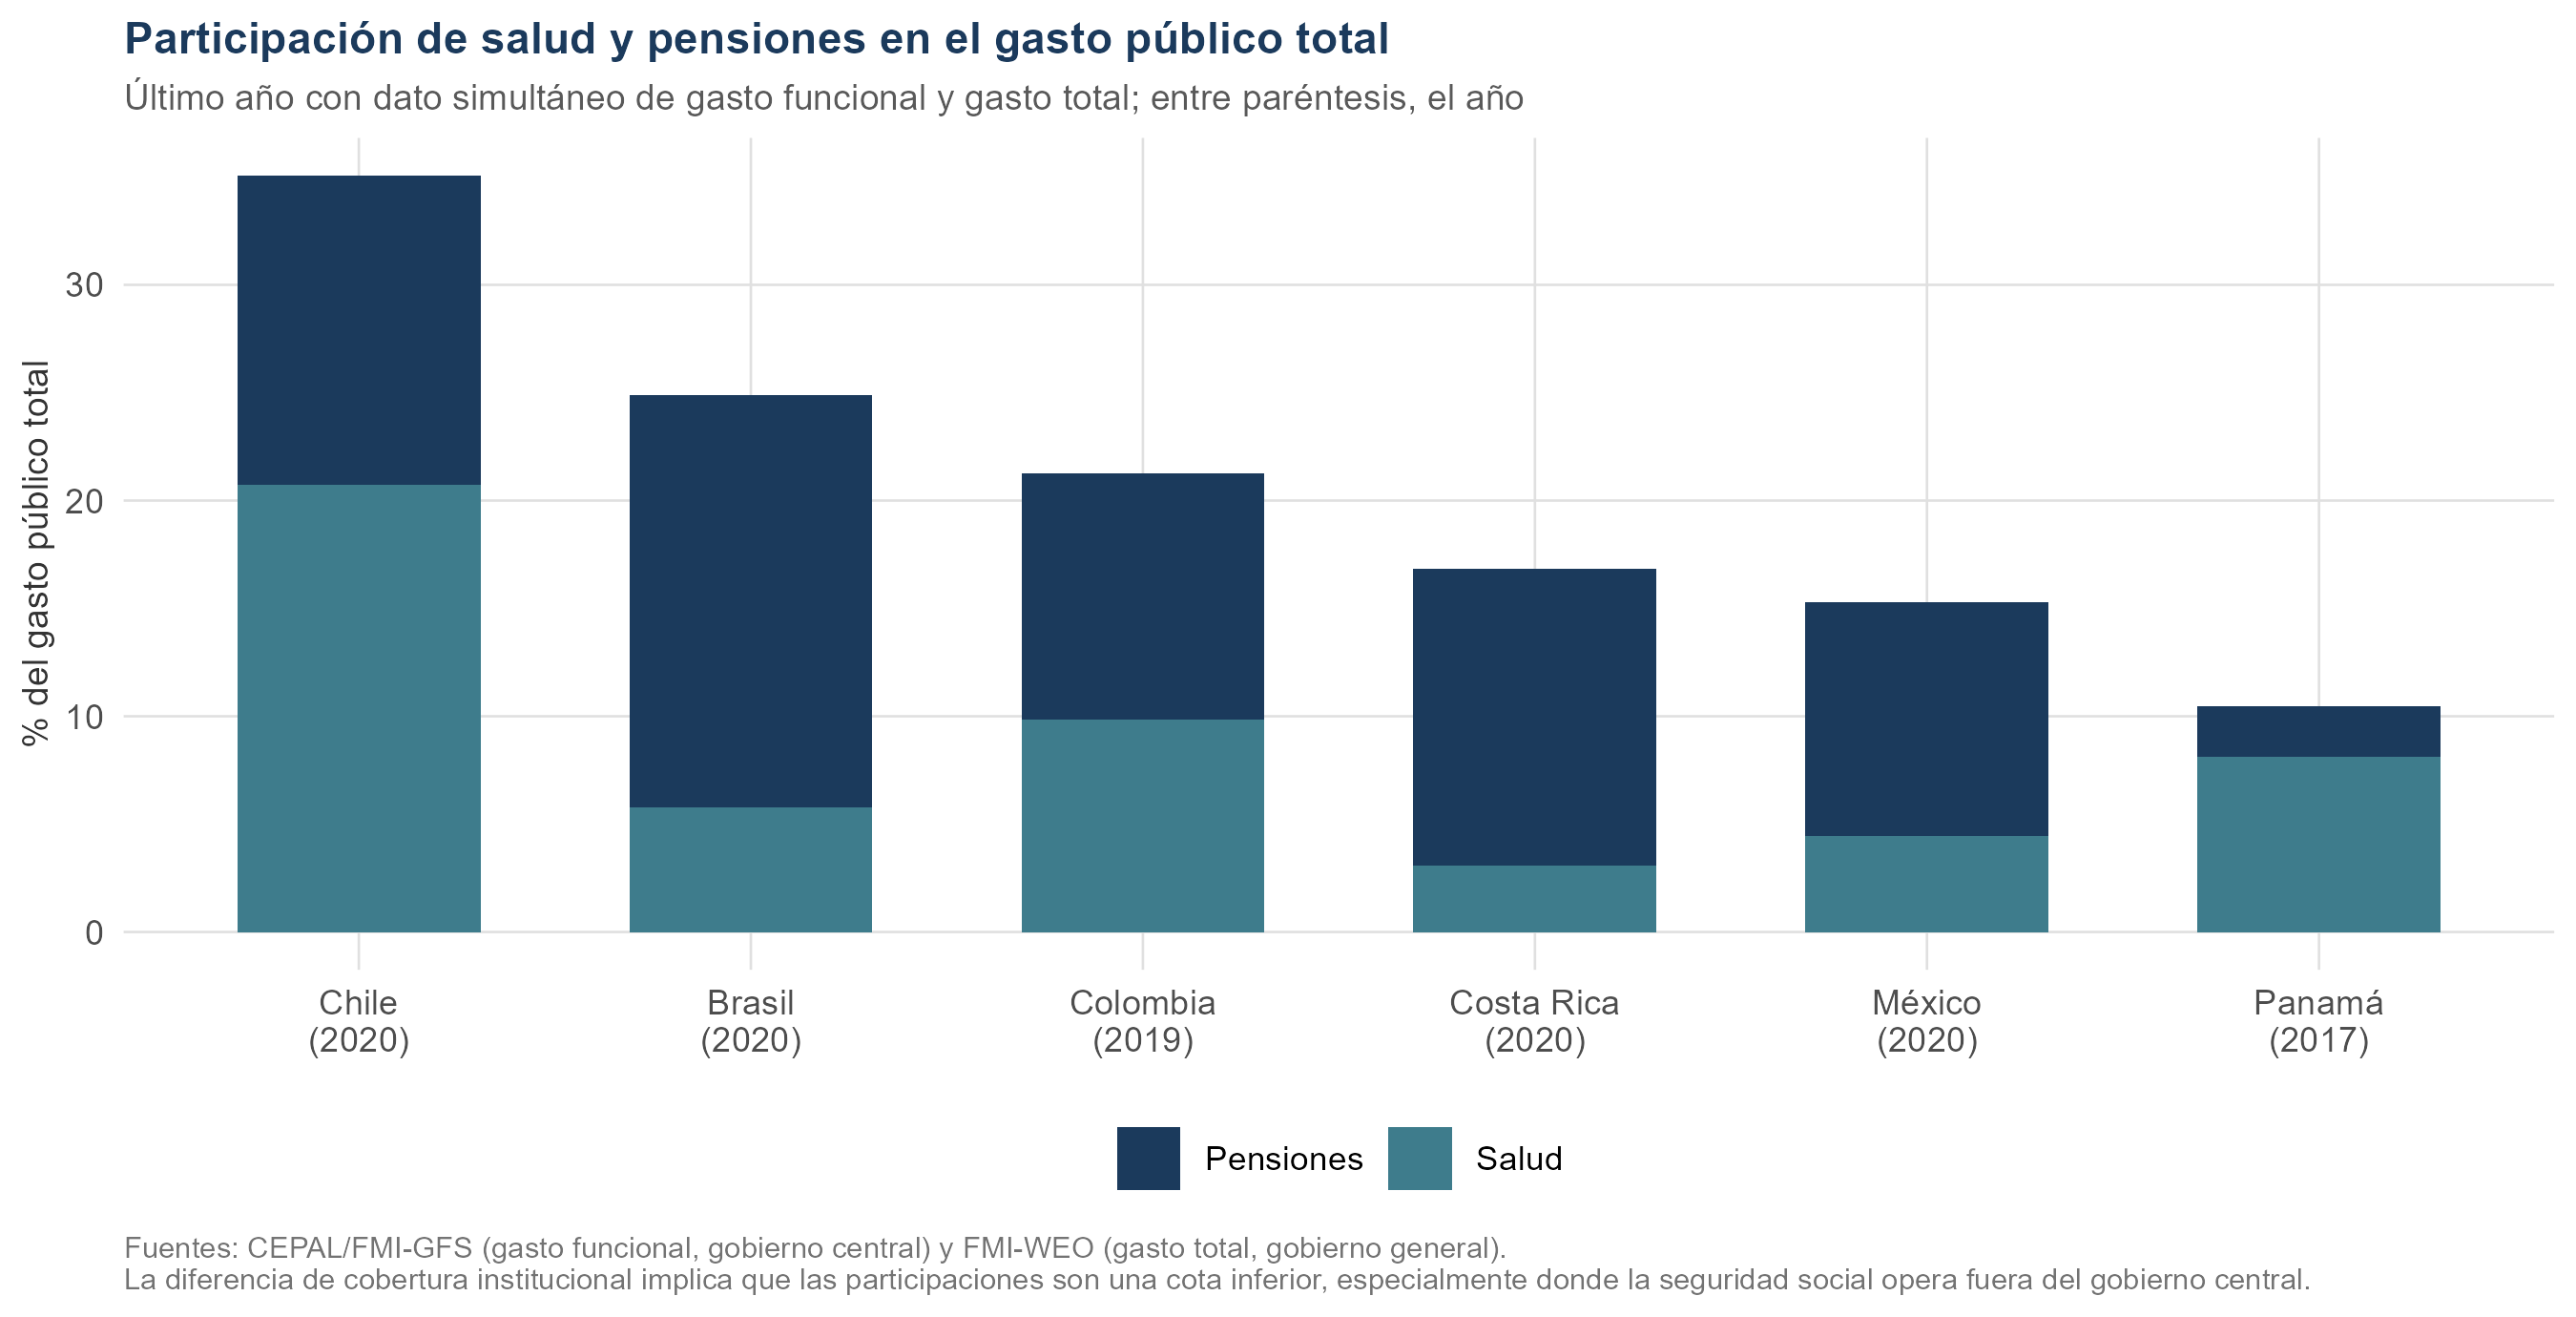
\includegraphics[width=0.92\textwidth]{graficas/fig_composicion_gasto.png}
  \caption{Participación de salud y pensiones en el gasto público total,
  último año con dato simultáneo.}
  \label{fig:composicion}
\end{figure}

Tres lecturas se desprenden. Primero, Chile y Brasil destinan a estas dos funciones
una fracción del presupuesto notablemente superior al resto —35,1 y 24,9\,\%
respectivamente— y son también, junto con Costa Rica, los países en etapa más avanzada
de la transición demográfica. La correspondencia entre etapa demográfica y rigidez
presupuestaria es el mecanismo central que este documento busca cuantificar.

Segundo, la composición interna difiere de manera reveladora. En Chile domina el
componente de salud (20,7\,\% del gasto frente a 14,3\,\% de pensiones), coherente con
un sistema de pensiones de capitalización individual en el que el pasivo previsional no
transita por el presupuesto público en la misma magnitud que en un régimen de reparto.
En Brasil ocurre lo contrario: pensiones representa 19,1\,\% del gasto frente a 5,8\,\%
de salud, reflejo directo del RGPS/RPPS de reparto y beneficio definido descrito en la
Sección~\ref{sec:brasil}.

Tercero, las cifras bajas de Costa Rica y Panamá deben leerse contemplando la limitación en cobertura ya señalada. En ambos casos el grueso del financiamiento de salud y pensiones
transita por instituciones de seguridad social —CCSS y CSS— que no forman parte del gobierno central, de modo que la participación reportada es una cota inferior. 

% ---------------------------------------------------------------------
\subsection{Proyecciones fiscales}
\label{sec:proyecciones}
% ---------------------------------------------------------------------

\subsubsection{Procedimiento}
\label{sec:procedimiento}

Las proyecciones se construyen mediante un procedimiento univariado uniforme para las treinta series fiscales (cinco indicadores por seis países), con selección de modelo
basada en desempeño fuera de muestra. La elección de un enfoque univariado responde al
alcance de este producto: el objetivo es caracterizar la inercia de cada serie, no
estimar elasticidades estructurales.

El procedimiento consta de cuatro etapas. En la primera se determina el orden de integración de cada serie mediante las pruebas de Dickey-Fuller aumentada
(H$_0$: raíz unitaria) y KPSS (H$_0$: estacionariedad), sintetizadas en el criterio
\texttt{ndiffs} \citep{hyndman2021}. La evidencia sobre datos anuales es la esperable para series fiscales: los agregados de nivel —ingresos, deuda neta, gasto en
salud y en pensiones— requieren en general una diferencia regular por presentar tendencia estocástica, mientras que el balance primario resulta estacionario o próximo
a serlo, consistente con su naturaleza de flujo que revierte alrededor de cero. Esta
diferencia de comportamiento entre indicadores es relevante: implica que la deuda neta
y el gasto funcional son series con memoria larga, en las que un choque desplaza el
nivel de forma persistente, mientras que el balance primario tiende a retornar a su
media tras una perturbación. La Tabla~\ref{tab:integracion} resume el resultado por
indicador.

\begin{table}[htbp]
  \centering
  \caption{Orden de integración sugerido (\texttt{ndiffs}): número de países por
  indicador.}
  \label{tab:integracion}
  
\begin{tabular}{lrrr}
\toprule
Indicador & d = 0 & d = 1 & d = 2\\
\midrule
Balance primario & 2 & 4 & 0\\
Deuda neta del gobierno general & 2 & 4 & 0\\
Gasto público en pensiones & 1 & 5 & 0\\
Gasto público en salud & 1 & 4 & 1\\
Ingresos del gobierno general & 3 & 3 & 0\\
\bottomrule
\end{tabular}

  \vspace{2pt}
  \footnotesize
  $d$: número de diferencias regulares requeridas según la combinación de las
  pruebas ADF y KPSS. Elaboración propia.
\end{table}

En la segunda etapa se estiman tres familias de modelo sobre cada serie. ARIMA, bajo
la metodología Box-Jenkins con selección de órdenes por AICc mediante búsqueda
exhaustiva, incorpora la diferenciación de forma endógena y captura la estructura
autorregresiva y de medias móviles. ETS, con selección automática de componentes por
máxima verosimilitud, modela nivel y tendencia de manera explícita sin requerir
estacionariedad previa, lo que le confiere ventaja en series cortas. Holt con
amortiguación introduce un parámetro que atenúa progresivamente la pendiente
proyectada; su inclusión responde a una consideración sustantiva y no meramente
técnica: en horizontes de diez años, una extrapolación lineal de la tendencia reciente
produce trayectorias implausibles para razones acotadas como las aquí analizadas, y la
amortiguación impone una convergencia gradual que resulta más congruente con el
comportamiento observado de los agregados fiscales.

En la tercera etapa se reserva una ventana de cuatro años de cada serie como
conjunto de validación y se selecciona, para cada una, el modelo con menor raíz del
error cuadrático medio fuera de muestra. Para los agregados del WEO, que llegan a
2024, la ventana son los últimos cuatro años observados (2021--2024). Para las
series de gasto funcional la ventana son los cuatro años \emph{anteriores a 2020}
(2016--2019): en la versión intermedia de este documento la validación incluía el
año del choque sanitario y la selección favorecía especificaciones de tendencia no
amortiguada que extrapolaban el incremento de 2020 como si fuera estructural, lo
que el control de rango del propio procedimiento detectó en tres series. Excluir
2020 de la validación ---no de la estimación final--- corrige la selección en la
serie de pensiones de México, donde la proyección converge ahora a
3{,}0\,\% del PIB en lugar de escalar a 5{,}3\,\%; en las series de salud de Chile y
de México la selección no cambia de forma que apague el control de rango, y sus
trayectorias conservan la advertencia textual que las acompaña. Se reporta
adicionalmente el error absoluto medio escalado (MASE). La cuarta etapa reestima el
modelo seleccionado sobre la muestra completa ---incluido 2020 donde existe--- y
proyecta a diez años, validando la especificación mediante la prueba de Ljung-Box
sobre los residuales (H$_0$: ausencia de autocorrelación).

El criterio de selección se aplica serie por serie y no de forma agregada. Esta decisión es deliberada: aplicar una única especificación a las treinta series por
conveniencia operativa —típicamente ARIMA automático— ignoraría que las series con
tendencia dominante y muestra corta se ajustan mejor mediante suavizamiento exponencial,
y que un ARIMA cuyos residuales conservan autocorrelación produce intervalos de
pronóstico mal calibrados. La Tabla~\ref{tab:modelos} documenta la especificación
seleccionada para cada serie y su desempeño.

\begin{table}[htbp]
  \centering
  \caption{Modelo seleccionado por serie, desempeño fuera de muestra y diagnóstico
  de residuales.}
  \label{tab:modelos}
  \begin{adjustbox}{max width=\textwidth}
  
\begin{tabular}{lrrrrrrrr}
\toprule
Indicador & País & n & Modelo & RMSE & MASE & Ljung-Box (p) & Ventana & Figura\\
\midrule
Ingresos del gobierno general & Brasil & 24 & ETS & 1.704 & 1.13 & 0.657 & 2021-2024 & sí\\
Ingresos del gobierno general & Chile & 25 & ARIMA & 3.097 & 2.24 & 0.961 & 2021-2024 & no (n.i.)\\
Ingresos del gobierno general & Colombia & 25 & ETS & 2.476 & 1.63 & 0.233 & 2021-2024 & sí\\
Ingresos del gobierno general & Costa Rica & 25 & ETS & 1.644 & 2.89 & 0.988 & 2021-2024 & no (n.i.)\\
Ingresos del gobierno general & México & 25 & ETS & 0.696 & 0.77 & 0.406 & 2021-2024 & sí\\
Ingresos del gobierno general & Panamá & 25 & Holt amortiguado & 0.744 & 0.49 & 0.638 & 2021-2024 & sí\\
Balance primario & Brasil & 24 & Holt amortiguado & 5.358 & 4.23 & 0.866 & 2021-2024 & no (n.i.)\\
Balance primario & Chile & 25 & Holt amortiguado & 5.329 & 2.37 & 0.696 & 2021-2024 & no (n.i.)\\
Balance primario & Colombia & 25 & ETS & 2.153 & 1.63 & 0.498 & 2021-2024 & sí\\
Balance primario & Costa Rica & 25 & ETS & 4.928 & 5.59 & 0.922 & 2021-2024 & no (n.i.)\\
Balance primario & México & 25 & Holt amortiguado & 0.555 & 0.53 & 0.312 & 2021-2024 & sí\\
Balance primario & Panamá & 25 & ETS & 5.025 & 3.26 & 0.134 & 2021-2024 & no (n.i.)\\
Deuda neta del gobierno general & Brasil & 24 & ARIMA & 3.904 & 0.95 & 0.623 & 2021-2024 & sí\\
Deuda neta del gobierno general & Chile & 25 & Holt amortiguado & 3.099 & 0.89 & 0.400 & 2021-2024 & sí\\
Deuda neta del gobierno general & Colombia & 25 & ETS & 3.220 & 0.66 & 0.284 & 2021-2024 & sí\\
Deuda neta del gobierno general & Costa Rica & 14 & Holt amortiguado & 36.586 & 7.38 & 0.534 & 2021-2024 & no (n.i.)\\
Deuda neta del gobierno general & México & 25 & ETS & 2.299 & 1.01 & 0.441 & 2021-2024 & sí\\
Deuda neta del gobierno general & Panamá & 25 & ETS & 3.480 & 0.77 & 0.631 & 2021-2024 & sí\\
Gasto público en salud & Brasil & 31 & Holt amortiguado & 0.188 & 1.49 & 0.657 & 2016-2019 & sí\\
Gasto público en salud & Chile & 31 & ARIMA & 0.210 & 1.28 & 0.441 & 2016-2019 & sí\\
Gasto público en salud & Colombia & 30 & ETS & 0.355 & 2.28 & 0.830 & 2016-2019 & no (n.i.)\\
Gasto público en salud & Costa Rica & 28 & ETS & 0.025 & 0.27 & 0.273 & 2016-2019 & sí\\
Gasto público en salud & México & 22 & ETS & 0.131 & 2.09 & 0.830 & 2016-2019 & no (n.i.)\\
Gasto público en salud & Panamá & 18 & ETS & 0.176 & 0.55 & 0.967 & 2014-2017 & sí\\
Gasto público en pensiones & Brasil & 21 & ARIMA & 1.019 & 2.60 & 0.420 & 2016-2019 & no (n.i.)\\
Gasto público en pensiones & Chile & 31 & Holt amortiguado & 0.066 & 0.25 & 0.456 & 2016-2019 & sí\\
Gasto público en pensiones & Colombia & 14 & ARIMA & 0.405 & 1.57 & 0.783 & 2016-2019 & sí\\
Gasto público en pensiones & Costa Rica & 15 & Holt amortiguado & 0.098 & 1.00 & 0.742 & 2016-2019 & sí\\
Gasto público en pensiones & México & 22 & Holt amortiguado & 0.063 & 0.35 & 0.448 & 2016-2019 & sí\\
Gasto público en pensiones & Panamá & 14 & ETS & 0.065 & 0.78 & 0.952 & 2014-2017 & sí\\
\bottomrule
\end{tabular}
  \end{adjustbox}

  \vspace{2pt}
  \footnotesize
  RMSE y MASE calculados sobre la ventana de validación indicada en la columna
  \emph{Ventana}, excluida de la estimación en esa etapa. MASE inferior a la unidad
  indica desempeño superior al método ingenuo de persistencia; sobre la
  interpretación de los valores superiores a la unidad, véase la primera precisión
  de la Sección~\ref{sec:alcance-proy}. Ljung-Box: valor $p$ superior a 0.05 indica
  ausencia de autocorrelación residual. \emph{Figura}: ``no (n.i.)'' identifica las
  series con MASE superior a dos, que se consideran no informativas, se retiran de
  las figuras de proyección y se conservan en esta tabla y en la base de datos con
  esa marca. El balance primario no se grafica en ningún caso (véase el texto).
  Elaboración propia.
\end{table}

\subsubsection{Resultados}

Las Figuras~\ref{fig:proj-ingresos} a~\ref{fig:proj-pensiones} presentan las
trayectorias proyectadas de cuatro de los cinco indicadores. Cada panel identifica
en su encabezado el país y el modelo seleccionado, de modo que la especificación
que genera cada trayectoria resulta inmediatamente identificable. Los paneles
correspondientes a series con MASE superior a dos ---ingresos de Chile y Costa
Rica, deuda neta de Costa Rica, salud de Colombia y México, pensiones de Brasil---
se omiten de las figuras: su especificación no supera a la regla de persistencia y
la trayectoria dibujada no aportaría información. Sus filas se conservan en la
Tabla~\ref{tab:modelos} con la marca correspondiente. El balance primario no se
grafica en absoluto, y la razón merece explicitarse: es la única de las cinco
series que resulta estacionaria o próxima a serlo (Tabla~\ref{tab:integracion}),
revierte a una media cercana a cero por su naturaleza de flujo, y su extrapolación
univariada no aporta información más allá de esa media; cuatro de sus seis series
presentan, además, MASE superior a dos. La lectura informativa del balance primario
es la de su posición de 2024 (Tabla~\ref{tab:ultimo-weo}) y la de su brecha respecto
del nivel que estabiliza la deuda, que se calcula en la Sección~\ref{sec:espacio}.
Las proyecciones se presentan como estimación puntual,
sin banda de intervalo: la finalidad es exponer el escenario central y su ordenamiento
relativo entre países, no cuantificar la incertidumbre, que crece de forma sustancial
con el horizonte. La lectura de estas trayectorias como cotas y no como pronósticos
se desarrolla en la Sección~\ref{sec:alcance-proy}.

\begin{figure}[htbp]
  \centering
  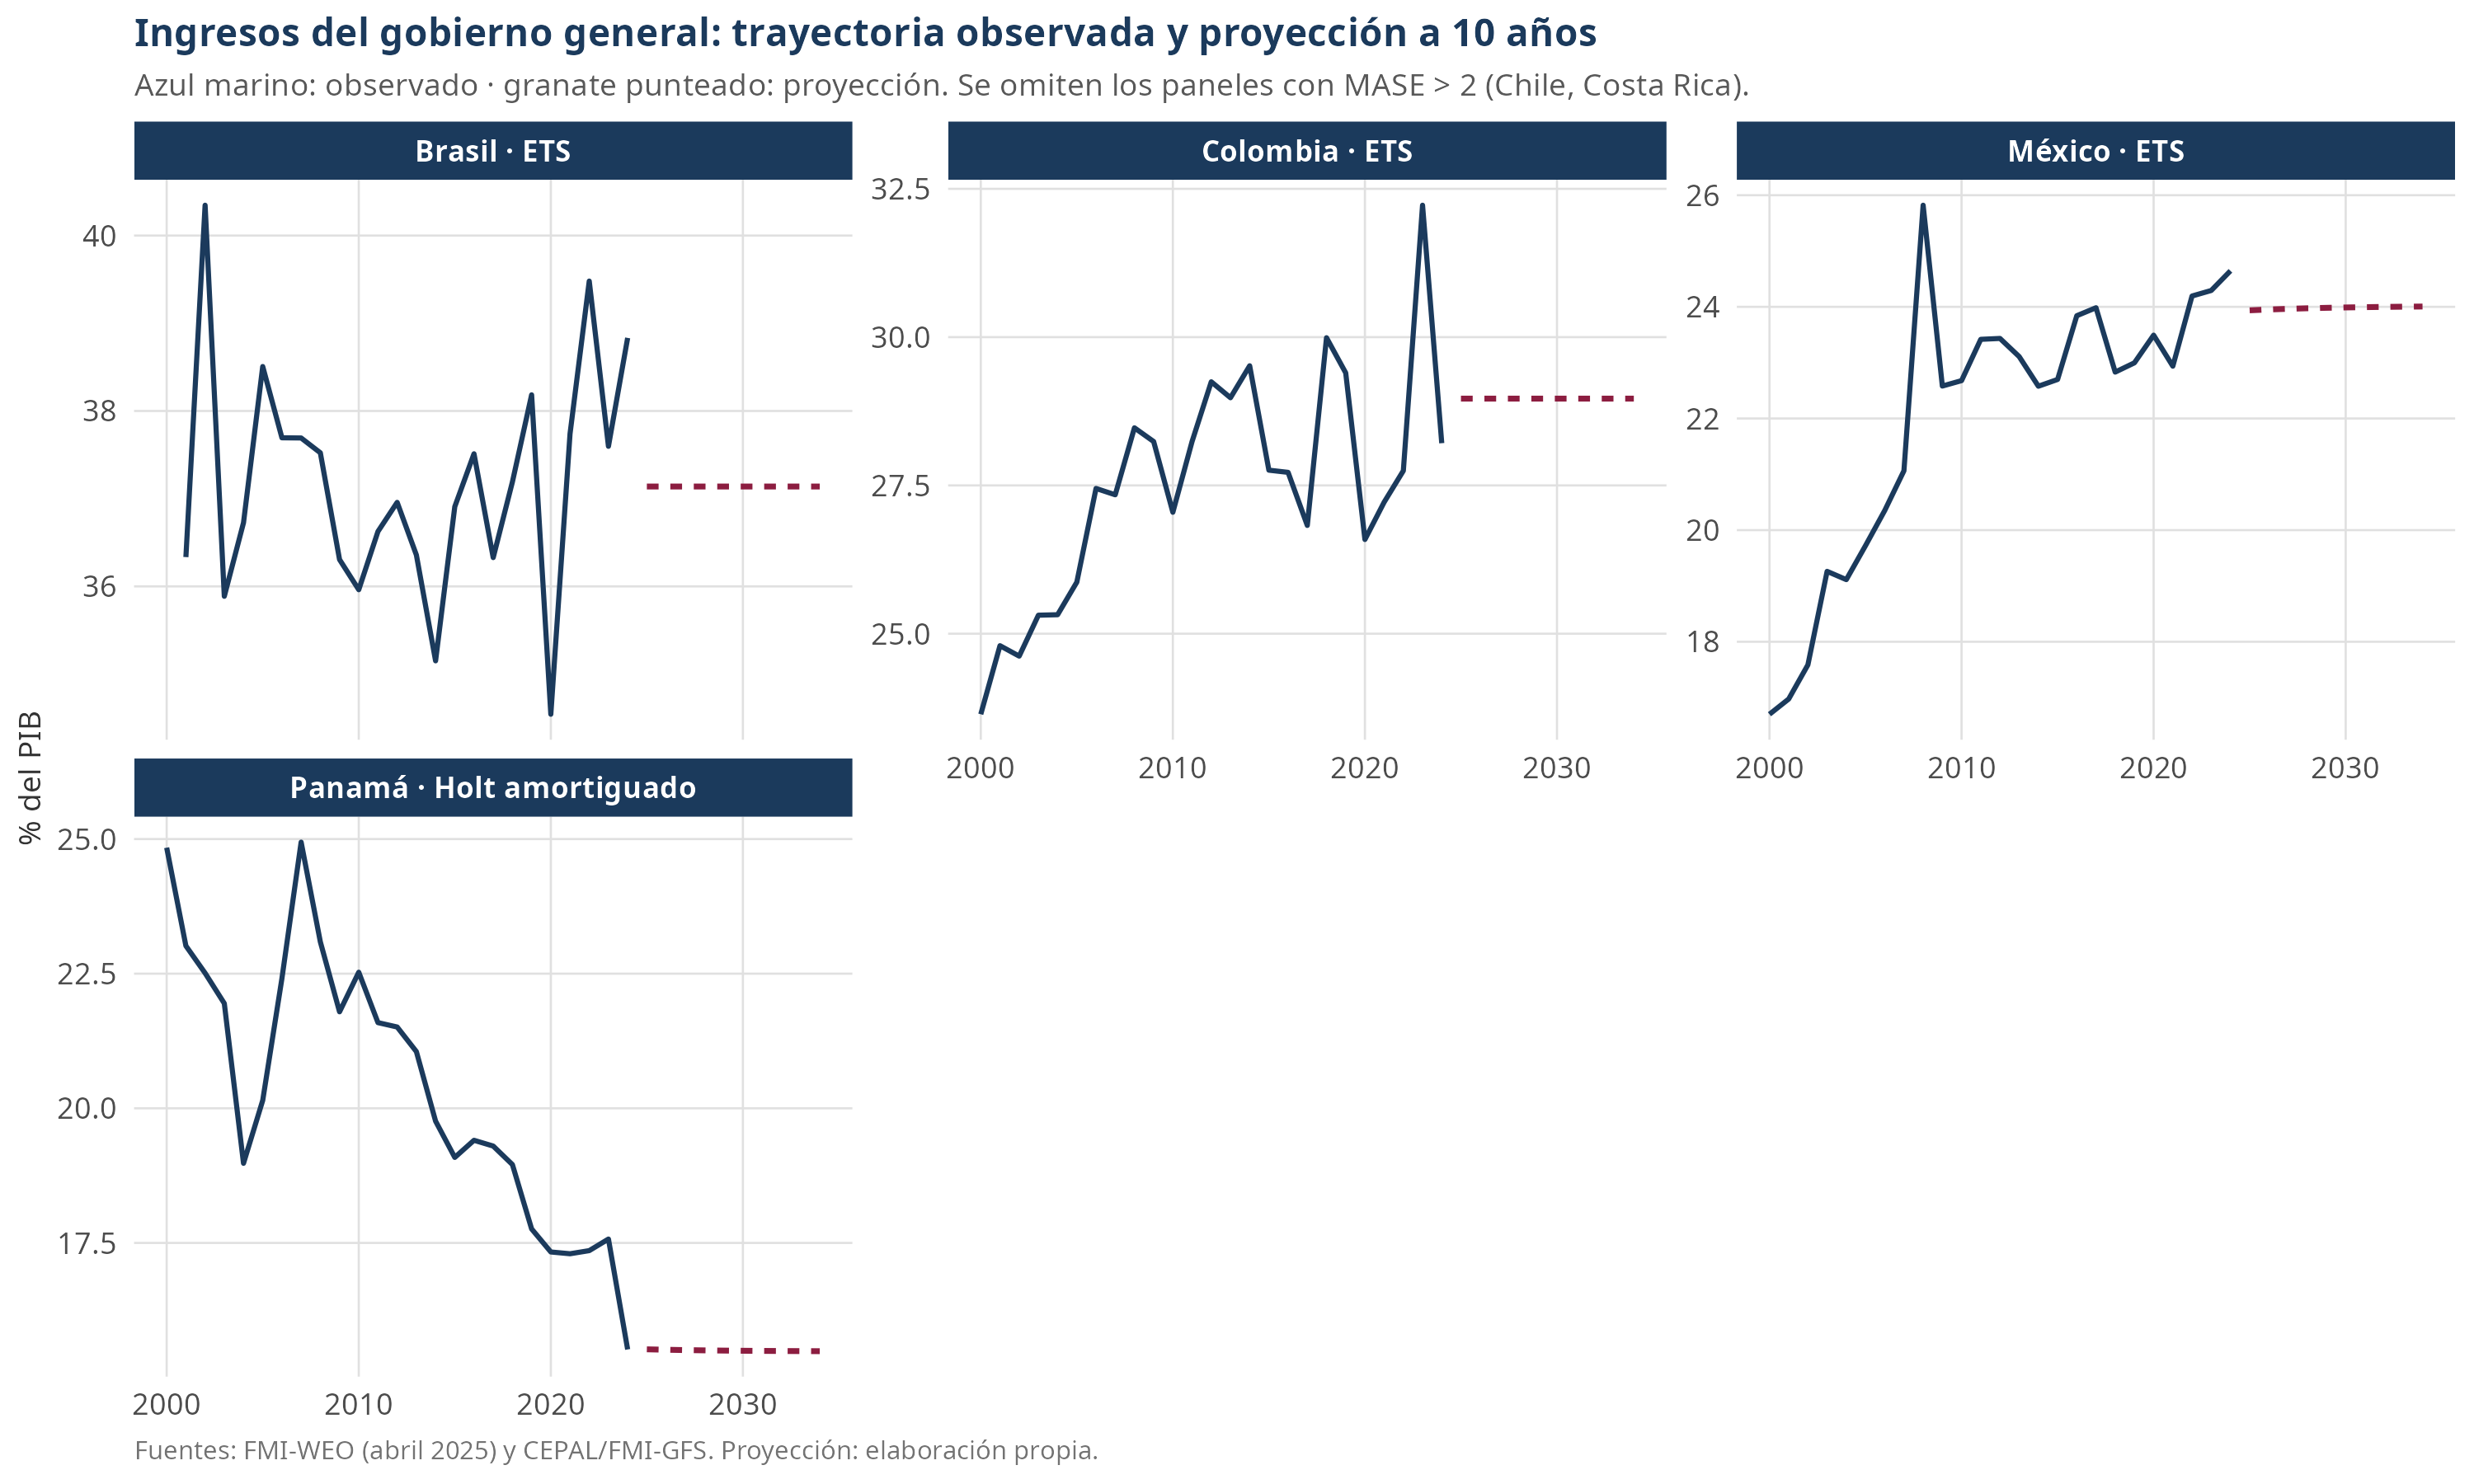
\includegraphics[width=\textwidth]{graficas/fig_proj_ingresos.png}
  \caption{Ingresos del gobierno general: trayectoria observada y proyección a diez
  años. Elaboración propia sobre FMI-WEO. Se omiten Chile y Costa Rica (MASE
  superior a dos).}
  \label{fig:proj-ingresos}
\end{figure}

\begin{figure}[htbp]
  \centering
  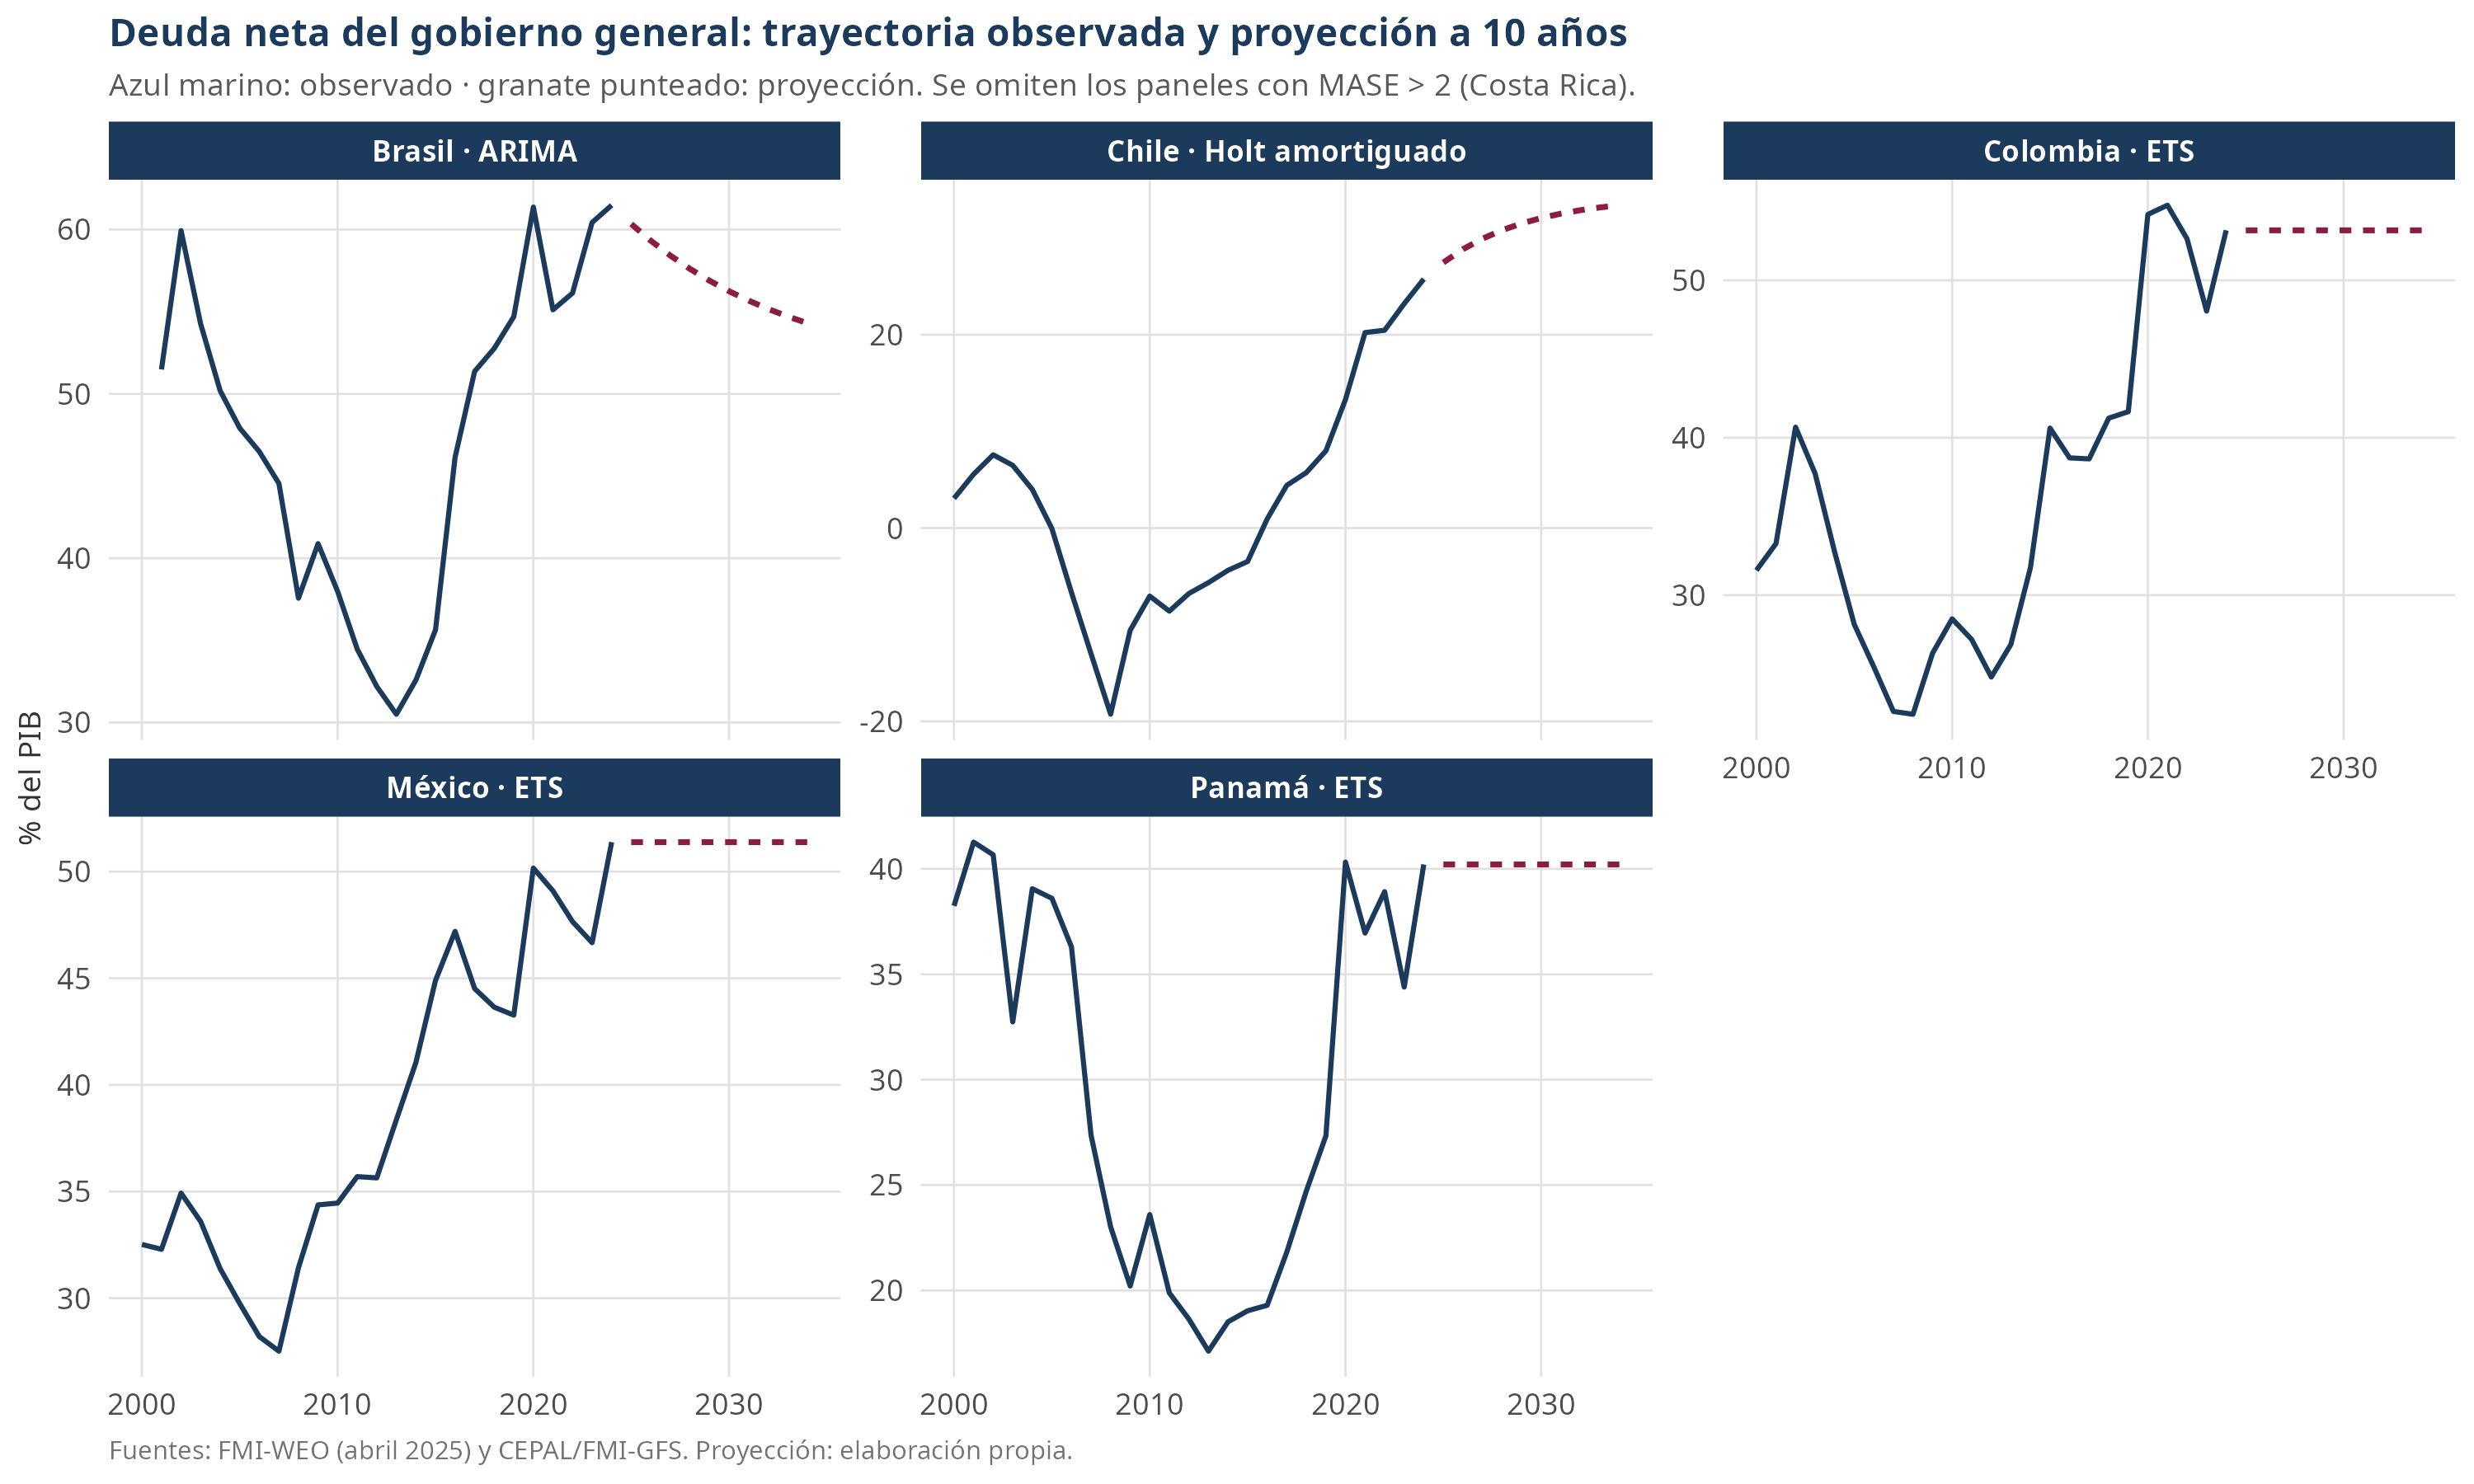
\includegraphics[width=\textwidth]{graficas/fig_proj_deuda.png}
  \caption{Deuda neta del gobierno general: trayectoria observada y proyección a diez
  años. Elaboración propia sobre FMI-WEO. Se omite Costa Rica (MASE superior a
  dos sobre catorce observaciones).}
  \label{fig:proj-deuda}
\end{figure}

\begin{figure}[htbp]
  \centering
  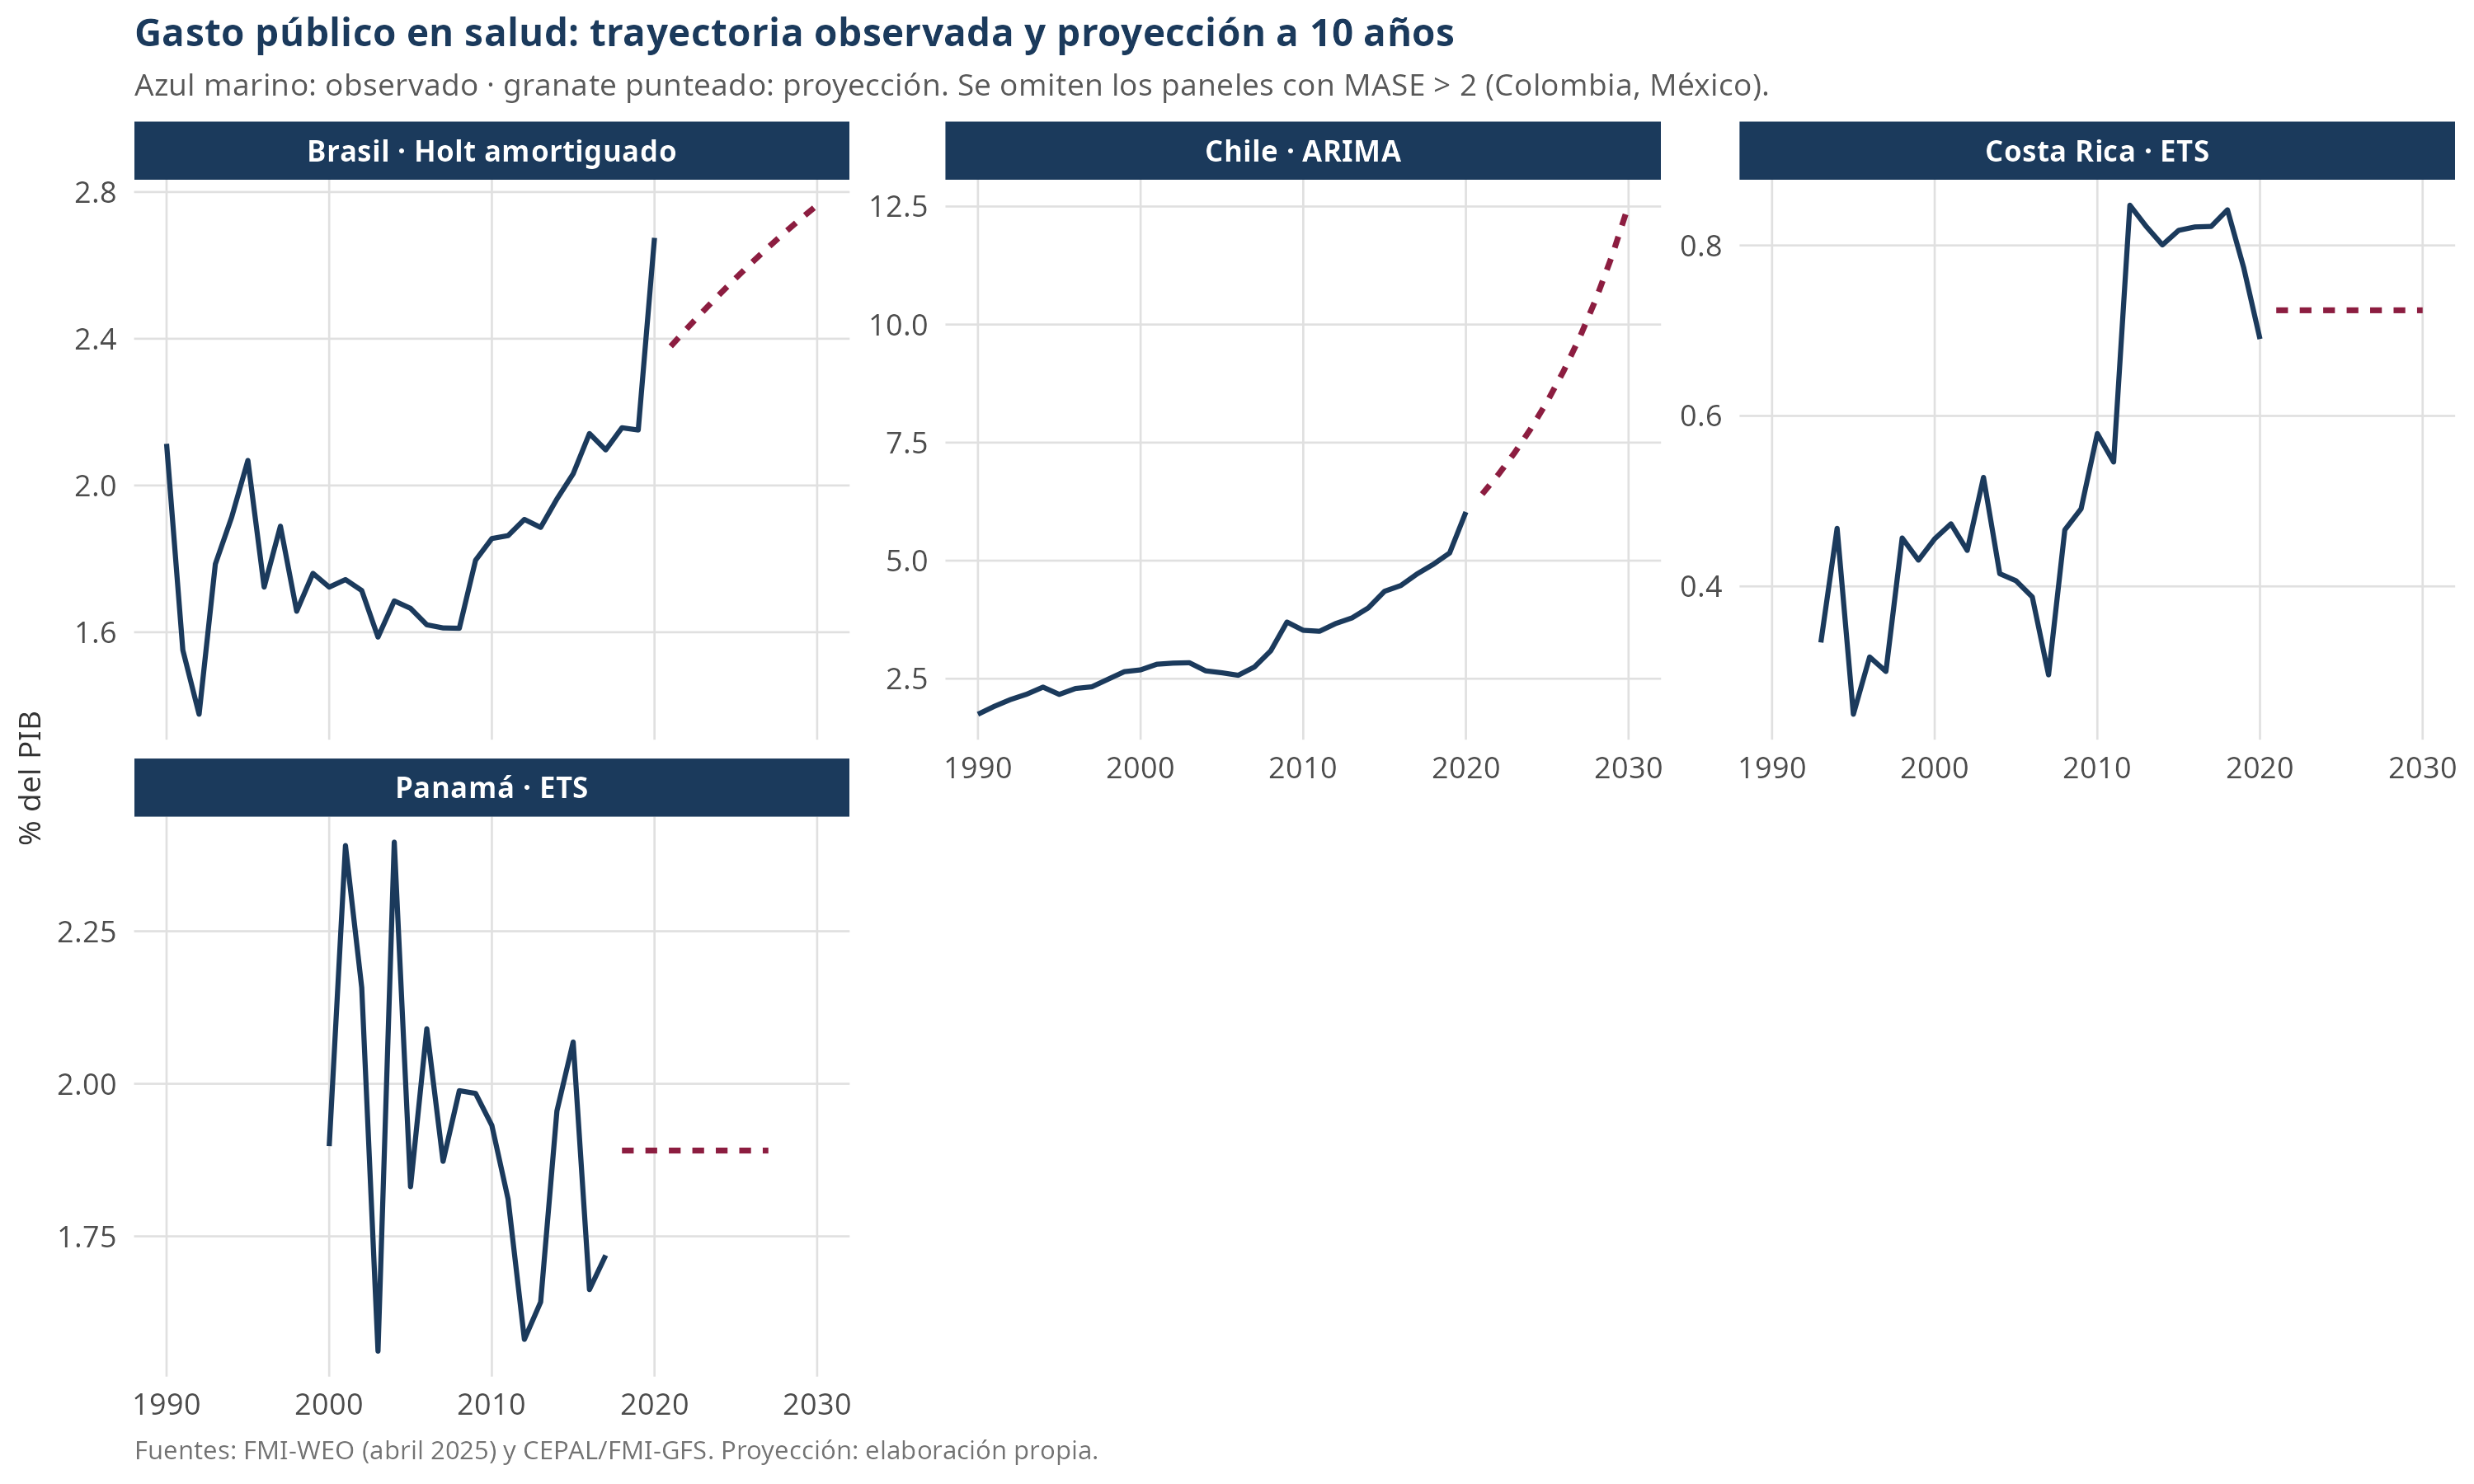
\includegraphics[width=\textwidth]{graficas/fig_proj_salud.png}
  \caption{Gasto público en salud: trayectoria observada y proyección a diez años.
  Elaboración propia sobre CEPAL/FMI-GFS. Se omiten Colombia y México (MASE
  superior a dos). La trayectoria proyectada para Chile ---que extiende el nivel
  observado de 6,0\,\% del PIB en 2020 hacia valores sustancialmente superiores al
  final del horizonte--- es resultado de la extrapolación de una tendencia
  histórica pronunciada y sostenida, sin restricción de plausibilidad ni
  amortiguación de la pendiente, y persiste tras excluir 2020 de la ventana de
  validación. Constituye una caracterización de la inercia de la serie, no un
  escenario de gasto, y el control de rango del procedimiento la señala como tal.}
  \label{fig:proj-salud}
\end{figure}

\begin{figure}[htbp]
  \centering
  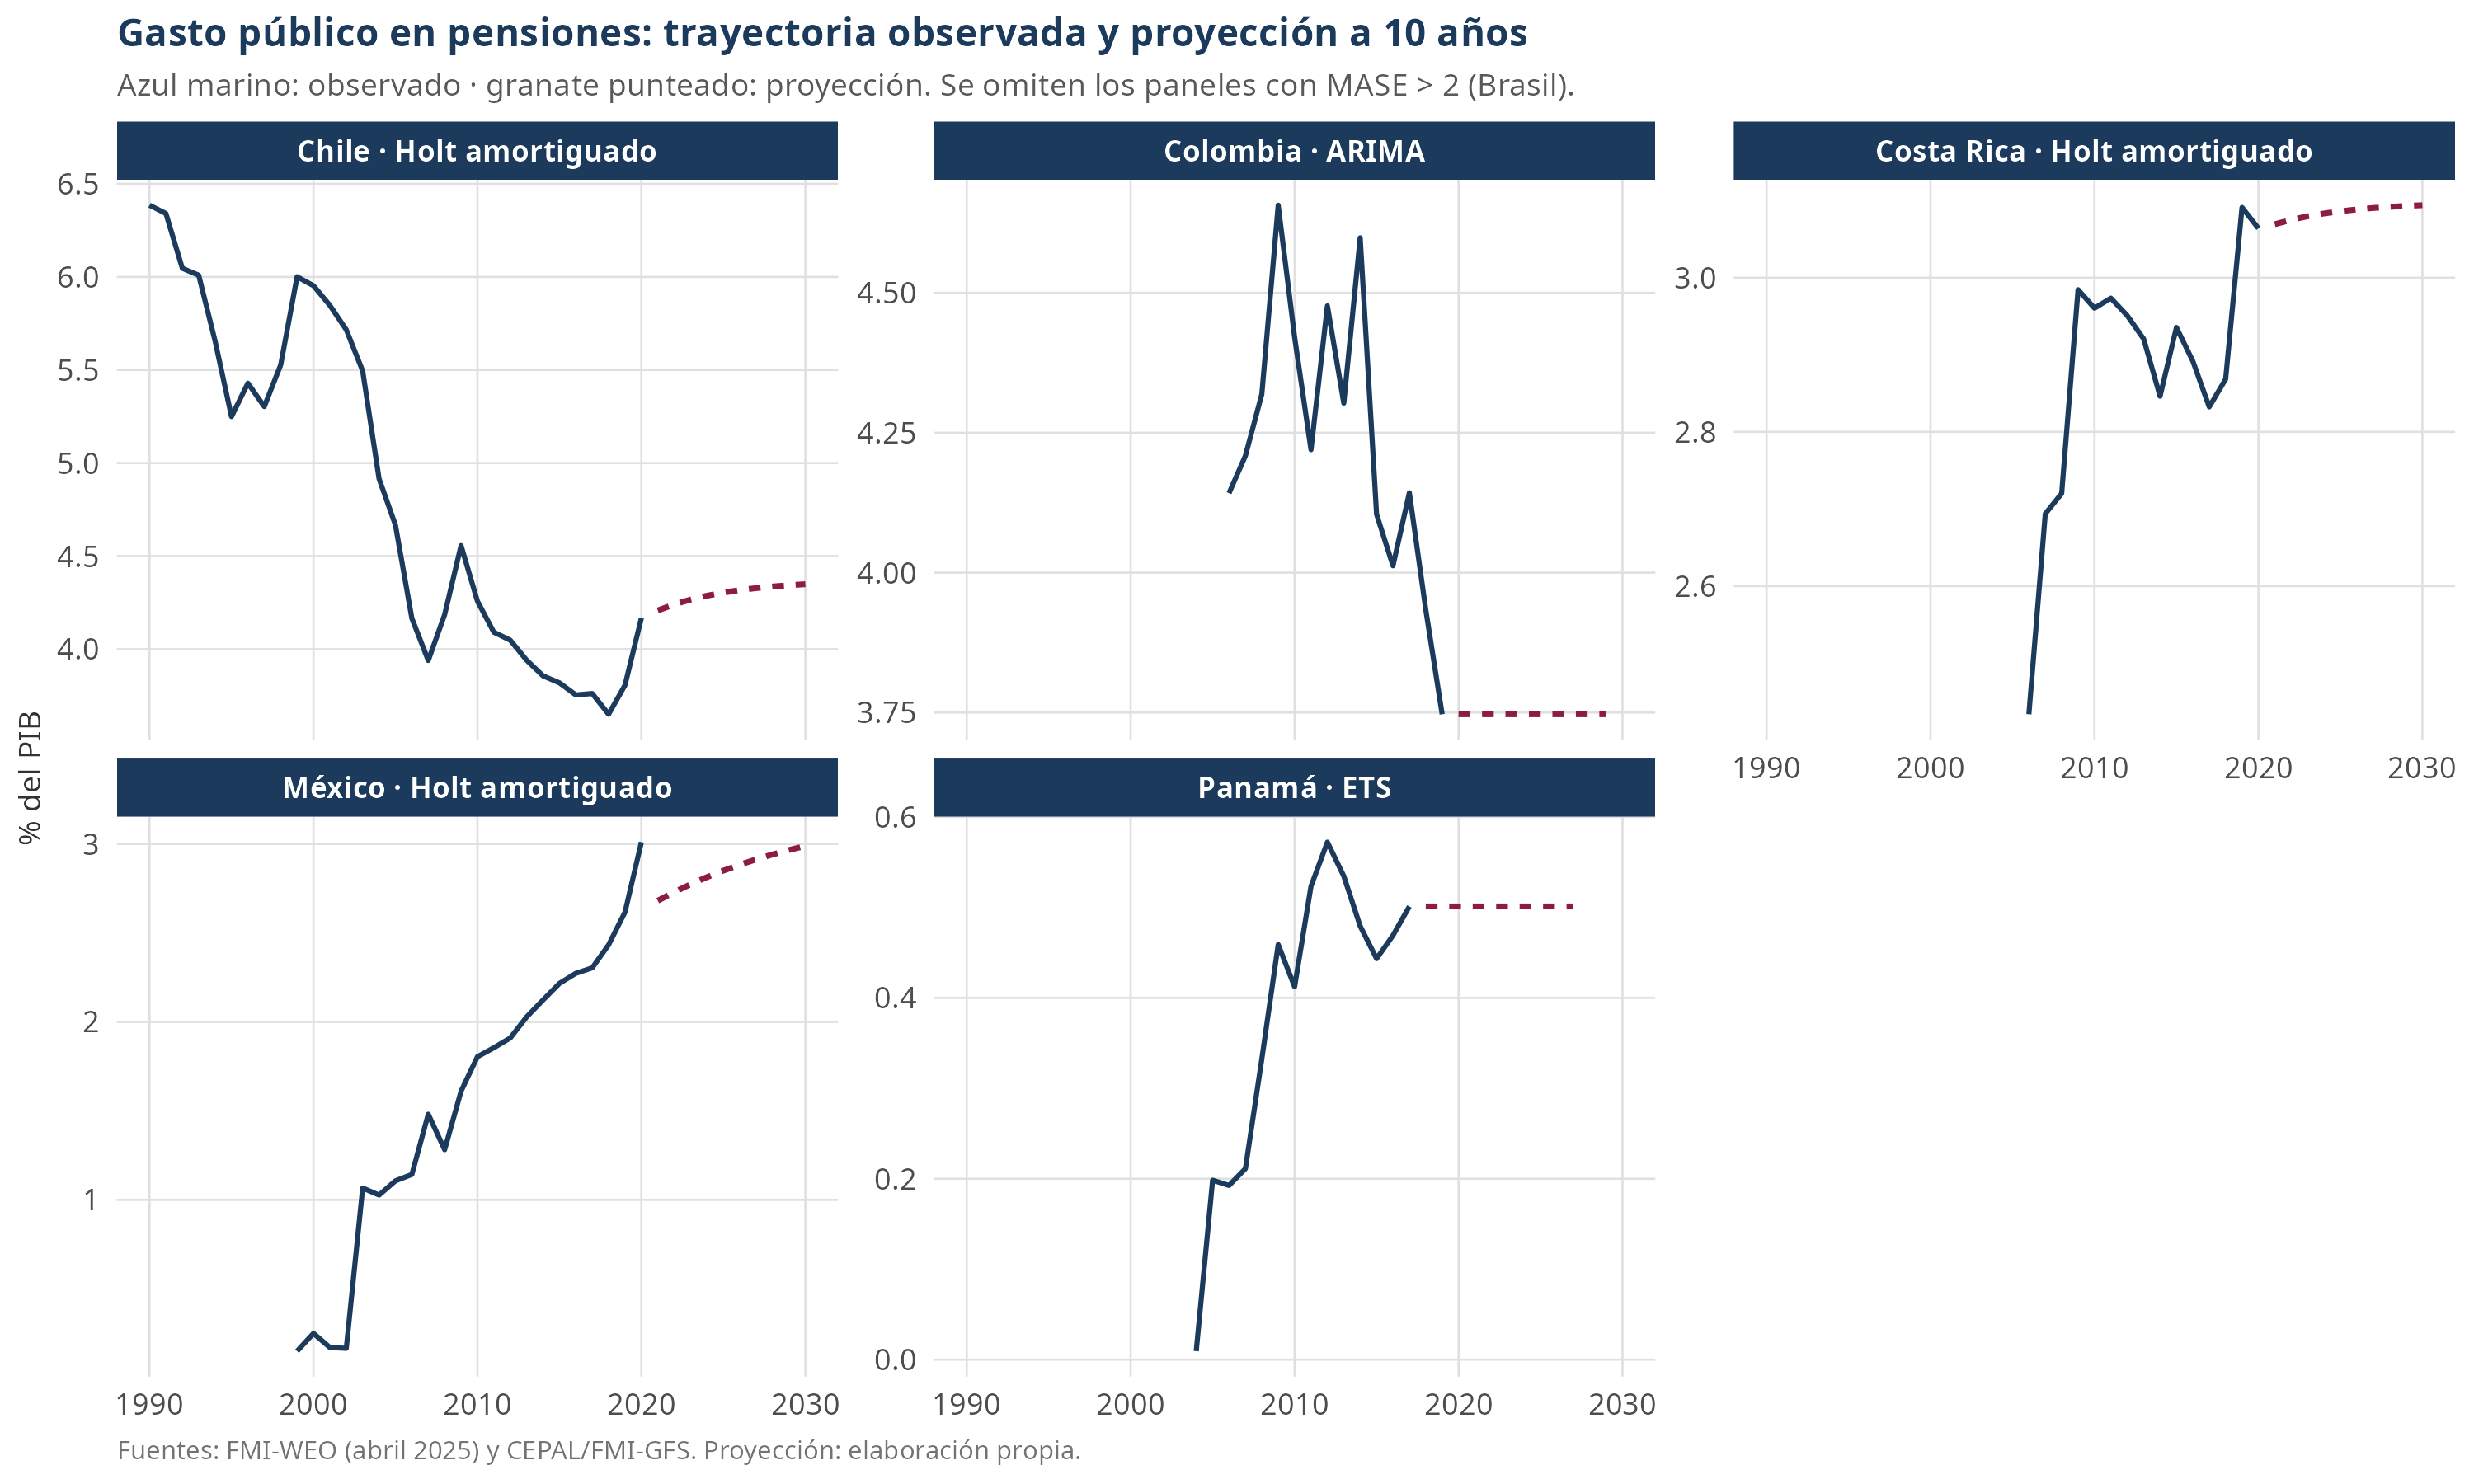
\includegraphics[width=\textwidth]{graficas/fig_proj_pensiones.png}
  \caption{Gasto público en pensiones: trayectoria observada y proyección a diez años.
  Elaboración propia sobre CEPAL/FMI-GFS. Se omite Brasil (MASE superior a dos).
  La proyección para México, seleccionada con ventana de validación anterior a
  2020, es ahora de tendencia amortiguada y converge a 3{,}0\,\% del PIB; la serie
  histórica refleja la maduración del régimen de transición documentada en la
  Sección~\ref{sec:mexico}, cuyo agotamiento previsible por cohorte no incorpora
  ningún modelo univariado.}
  \label{fig:proj-pensiones}
\end{figure}

\subsubsection{Alcance e interpretación}
\label{sec:alcance-proy}

Cuatro precisiones delimitan el alcance de estas proyecciones. La primera y más
importante concierne al desempeño desigual de los modelos entre series. El error
absoluto medio escalado (MASE) reportado en la Tabla~\ref{tab:modelos} compara cada
modelo con el método ingenuo de persistencia: un valor superior a la unidad indica
que la especificación seleccionada no supera a la regla de suponer que la serie
mantiene su último valor observado. Ese es el caso en poco más de la mitad de las
treinta series. En diez de ellas la discrepancia es de una magnitud que las
inhabilita como estimación puntual: la deuda neta de Costa Rica, estimada sobre
catorce observaciones, arroja un MASE de 7,38 y una raíz del error cuadrático medio
de 36,6 puntos del PIB; el balance primario de Costa Rica (5,59), Brasil (4,23),
Panamá (3,26) y Chile (2,37) muestra un patrón análogo, igual que los ingresos de
Costa Rica (2,89) y Chile (2,24), el gasto en salud de Colombia (2,28) y México
(2,09) y el gasto en pensiones de Brasil (2,60). \textbf{Las series con MASE
superior a dos se consideran no informativas: se retiran de las figuras de
proyección, se conservan en la Tabla~\ref{tab:modelos} y en la base de datos con
esa marca, y no deben leerse como pronóstico ni citarse como estimación puntual.}
La lectura informativa de este ejercicio se concentra en las series de nivel con
memoria larga ---deuda neta, ingresos y gasto funcional--- en los países donde la
muestra es suficiente. Debe añadirse una advertencia específica sobre las dos
series de salud que, con MASE inferior a dos, siguen excediendo el rango histórico
observado según el control automático del procedimiento: Chile (de 6,0 a 12,5\,\% del
PIB al final del horizonte) y, en menor medida, México. Se conservan con su
advertencia textual porque ninguna de las dos correcciones ensayadas ---ventana de
validación anterior a 2020 y restricción a especificaciones amortiguadas--- apagó
la alerta, y forzar una tercera habría sustituido un criterio uniforme por uno
\emph{ad hoc}. Deben leerse como cota superior de un escenario inercial, no como
estimación central.

La segunda es de naturaleza metodológica: al tratarse de modelos univariados, las
trayectorias extrapolan la inercia de cada serie sin incorporar la demografía como
determinante. Constituyen, por tanto, un escenario inercial —qué ocurriría si cada
serie mantuviera su dinámica histórica— y no una proyección condicionada al
envejecimiento. La comparación entre este escenario inercial y la presión
demográfica documentada en las Secciones~\ref{sec:demografia}
y~\ref{sec:salud-envejecimiento} se realiza en la Sección~\ref{sec:riesgos} por la
vía de la estática comparada ---incremento mecánico del gasto por cambio en la
estructura por edades---, no mediante modelos de series de tiempo con determinantes
demográficos explícitos, que quedan fuera del alcance de este documento.

La tercera es de cobertura temporal. Las series de gasto funcional terminan entre 2017
y 2020, de modo que sus proyecciones parten de una base anterior a la normalización
posterior a la pandemia y no incorporan la información fiscal más reciente. Esta
asimetría respecto a los agregados del WEO —que llegan a 2024— debe considerarse al
comparar trayectorias entre indicadores. Adicionalmente, dado que las series de
gasto funcional terminan entre 2017 y 2020, un horizonte de proyección de diez años
cubre en parte años ya transcurridos. El tramo inicial de esas trayectorias no es
pronóstico sino reconstrucción inercial de un período observable por otras fuentes.

La cuarta concierne a la estabilidad paramétrica. Las series fiscales de la región
presentan quiebres estructurales asociados a reformas tributarias, ciclos de
precios de materias primas y al choque de 2020. Esta afirmación tiene ahora
contenido empírico: el Apéndice~\ref{ap:tecnico} aplica a las treinta series la
prueba supF de constancia de parámetros y el procedimiento de Bai-Perron, y
encuentra que veintidós de las veinticinco series evaluables rechazan la constancia
de la media al 5\,\%, con fechas de quiebre que se concentran en 2004--2005,
2008--2010 y 2019--2020. Los modelos aquí empleados no incorporan estos quiebres de
forma explícita, por lo que la extrapolación del pasado más lejano debe
interpretarse con cautela, particularmente en las series cuya dinámica reciente
difiere del promedio histórico.

Con estas salvedades, el ejercicio cumple su función dentro de la arquitectura del
estudio: establece el punto de partida cuantitativo y la trayectoria inercial sobre
los cuales la Sección~\ref{sec:riesgos} evalúa el impacto diferencial de la
transición demográfica bajo las distintas configuraciones institucionales
documentadas en las Secciones~\ref{sec:pensiones} y~\ref{sec:salud}.







\newpage
% =======================================================================
\section{Análisis heurístico de riesgos macrofiscales}
\label{sec:riesgos}
% =======================================================================

\subsection{Marco del análisis}
\label{sec:marco-riesgos}

Por riesgo macrofiscal demográfico se entiende aquí la probabilidad de que la
transición demográfica, mediada por la arquitectura institucional de cada país,
obligue a un ajuste fiscal de magnitud o velocidad que la posición de partida no
puede absorber sin deterioro de la sostenibilidad de la deuda o sin recorte de otras
funciones del gasto. El análisis que sigue es \emph{heurístico} y no actuarial. No
proyecta sistema por sistema con reglas paramétricas y cohortes, ni cuantifica
pasivos previsionales. Ordena la exposición relativa de los seis países combinando
tres dimensiones que el documento ya documentó por separado: la arquitectura
institucional de pensiones y salud (Secciones~\ref{sec:pensiones}
y~\ref{sec:salud}), la presión demográfica (Secciones~\ref{sec:demografia}
y~\ref{sec:wpp}) y el espacio fiscal de partida
(Sección~\ref{sec:posicion-fiscal}). El resultado es un \textbf{ordenamiento
comparado}, no una cuantificación de pasivos, y debe leerse con esa modestia.

La elección del enfoque no es sólo una restricción de alcance. Un ejercicio
actuarial produce cifras precisas condicionadas a supuestos que, en seis países con
reformas en curso o suspendidas ---Colombia bajo el Auto A-841, Panamá bajo la Ley
462, Chile bajo la Ley 21.735---, tendrían vida corta. Un ordenamiento heurístico
sobre magnitudes observadas y una regla de conversión explícita es menos preciso
pero más robusto a esa inestabilidad, y es el tipo de información que un reporte
macroeconómico regional puede citar sin comprometerse con la calibración de un
modelo.

El eje que articula las tres dimensiones es el que la Sección~\ref{sec:sspsas}
dejó planteado: si el componente no contributivo opera como complemento o como
sustituto del contributivo. Esa pregunta determina por qué canal la demografía se
convierte en riesgo fiscal. Donde el Pilar 0 sustituye, el valor que el trabajador
atribuye a cotizar se reduce, la base contributiva se erosiona y el peso del
financiamiento se desplaza hacia las rentas generales precisamente cuando la razón
de dependencia se duplica. La literatura reciente sobre formalización en la región
muestra que la valoración que el trabajador hace del beneficio contributivo, junto
con la cuña tributaria y los costos de cumplimiento, es determinante de la decisión
de cotizar, y que esa valoración depende de la credibilidad de la promesa
previsional tanto como de su generosidad nominal \citep{wb2025}. En términos del
análisis de riesgo, esto significa que la presión demográfica no llega al fisco por
un solo canal: llega por el gasto (más beneficiarios) y por el ingreso (menos
cotizantes efectivos por cada trabajador en edad activa), y el diseño institucional
decide cuánto pesa cada uno.

\subsection{Espacio fiscal: la métrica}
\label{sec:espacio}

La métrica principal de espacio fiscal es la \textbf{brecha de balance primario
estabilizador de deuda}. Sea $b$ la deuda neta del gobierno general como
proporción del PIB, $r$ la tasa de interés implícita sobre esa deuda y $g$ el
crecimiento nominal del PIB. El balance primario que mantiene constante la razón de
deuda es
\begin{equation}
  pb^{*} = b \cdot \frac{r - g}{1 + g},
  \qquad\text{y la brecha es}\qquad
  \text{brecha} = pb^{*} - pb_{\text{observado}}.
  \label{eq:pbstar}
\end{equation}
Una brecha positiva mide, en puntos del PIB, el ajuste primario que el país tendría
que realizar para que su deuda neta dejara de crecer con la política actual; una
brecha negativa indica que el balance observado ya estabiliza o reduce la deuda. Es
la métrica de espacio fiscal más simple que conecta la fotografía de 2024 con la
restricción intertemporal, y es la que permite después preguntar qué fracción de
ese ajuste explica la demografía por sí sola.

\paragraph{Datos y supuestos.} La base de datos del documento contiene $b$ y $pb$
pero no el crecimiento nominal ni la tasa implícita. Ambos se obtuvieron de la
misma fuente y vintage que los agregados fiscales ---FMI, \emph{World Economic
Outlook}, abril de 2025--- y se incorporaron a la base con su tipo, fuente y
cobertura (Apéndice~\ref{ap:tecnico}): el crecimiento nominal como variación anual
del PIB a precios corrientes en moneda nacional, y el pago neto de intereses como
diferencia entre el balance primario y el balance global del gobierno general. La
tasa implícita es el pago neto de intereses del año dividido por la deuda neta del
año anterior. Para amortiguar el ruido de años individuales ---en particular el de
2020--2022, con caídas y rebotes del PIB nominal de dos dígitos--- el diferencial
$(r-g)$ se calcula sobre la ventana 2015--2024 como razón de sumas: la suma de
intereses pagados en la ventana sobre la suma de deuda neta inicial de cada año,
menos la media geométrica del crecimiento nominal. Como sensibilidad se reporta el
mismo cálculo sobre la proyección del propio WEO para 2025--2030. Los dos supuestos
que el lector debe tener presentes son que la tasa implícita histórica es la
relevante para el futuro y que $b$ es la deuda \emph{neta}, no la bruta.

\begin{table}[htbp]
  \centering
  \caption{Brecha de balance primario estabilizador de deuda, 2024 (\% del PIB;
  ordenada por brecha con ventana histórica).}
  \label{tab:espacio}
  \small
  \begin{tabular}{lrrrrrrrr}
\toprule
& & & \multicolumn{3}{c}{Ventana histórica 2015--2024} & \multicolumn{3}{c}{Proyección WEO 2025--2030} \\
\cmidrule(lr){4-6}\cmidrule(lr){7-9}
País & $b_{2024}$ & $pb_{2024}$ & $(r-g)$ & $pb^{*}$ & Brecha & $(r-g)$ & $pb^{*}$ & Brecha \\
\midrule
Panamá & 40.2 & $-$4.5 & 1.8 & 0.7 & \textbf{5.2} & 1.7 & 0.7 & 5.1 \\
Brasil & 61.5 & $-$0.3 & 4.8 & 2.8 & \textbf{3.1} & 4.2 & 2.4 & 2.8 \\
México & 51.4 & 0.2 & 3.5 & 1.7 & \textbf{1.5} & 4.2 & 2.0 & 1.8 \\
Chile & 25.8 & $-$2.0 & $-$2.4 & $-$0.6 & \textbf{1.4} & $-$1.4 & $-$0.3 & 1.6 \\
Costa Rica & 58.9 & 1.1 & 2.2 & 1.2 & \textbf{0.2} & 0.7 & 0.4 & $-$0.7 \\
Colombia & 53.2 & $-$0.8 & $-$1.6 & $-$0.8 & \textbf{0.0} & 1.2 & 0.6 & 1.4 \\
\bottomrule
\end{tabular}


  \vspace{2pt}
  \footnotesize
  $b_{2024}$: deuda neta del gobierno general; $pb_{2024}$: balance primario;
  $(r-g)$: diferencial entre tasa de interés implícita sobre deuda neta y
  crecimiento nominal del PIB, en puntos porcentuales; $pb^{*}$: balance primario
  estabilizador según la ecuación~\eqref{eq:pbstar}; brecha $= pb^{*} - pb_{2024}$.
  Ventana histórica: $r$ como razón de sumas 2015--2024, $g$ como media geométrica
  2015--2024. Proyección WEO: mismo cálculo sobre 2025--2030 con las proyecciones
  del FMI. \textbf{Advertencias.} El documento usa deuda \emph{neta}; la comparación
  internacional de $b$ es menos directa que con deuda bruta por la heterogeneidad
  en la valuación de activos (Sección~\ref{sec:posicion-fiscal}), y la tasa
  implícita sobre deuda neta es inestable cuando ésta es pequeña, como en Chile
  antes de 2018. Los valores de 2024 son estimación del FMI en Brasil, Costa Rica y
  Panamá, y observados en Chile, Colombia y México. Fuente: elaboración propia
  sobre FMI-WEO, abril de 2025.
\end{table}

La Tabla~\ref{tab:espacio} ordena los seis países. Tres lecturas se desprenden.

\textbf{Panamá y Brasil tienen las brechas mayores, por razones opuestas.} La
brecha panameña (5,2 puntos del PIB) proviene casi enteramente del déficit
primario de 2024 ($-4{,}5$\,\%), no de la dinámica de la deuda: su diferencial
$(r-g)$ es moderado (1,8 puntos) y su deuda neta es la tercera más baja del grupo.
La brecha brasileña (3,1 puntos) proviene en cambio del diferencial: con un pago
neto de intereses de 6,3\,\% del PIB en 2024 y una tasa implícita del orden de
12\,\% nominal, Brasil necesita un superávit primario cercano a 3\,\% del PIB para
estabilizar una deuda neta de 61,5\,\%, y registra un déficit de 0,3\,\%. Es la
única brecha del grupo cuya corrección exige sostener superávits primarios, no
sólo eliminar déficits.

\textbf{México y Chile ocupan una posición intermedia, con brechas de 1,5 y 1,4
puntos.} En México la brecha es de diferencial, como en Brasil, pero sobre una
deuda diez puntos menor y con balance primario ya en equilibrio. En Chile el
diferencial es negativo ---la tasa implícita sobre una deuda neta pequeña es
inferior al crecimiento nominal--- y la brecha proviene del déficit primario de
2024 ($-2{,}0$\,\%); es el único país del grupo que estabilizaría su deuda con un
déficit primario moderado, lo que refleja el activo que representan sus fondos
soberanos, descontados en la deuda neta.

\textbf{Costa Rica y Colombia no presentan brecha con la ventana histórica, y la
lectura debe ser cautelosa en ambos casos.} Costa Rica registra el mayor superávit
primario del grupo (1,1\,\%) y es el único país cuya deuda neta cayó en 2024; su
ajuste fiscal posterior a la regla fiscal de 2018 está hecho, y la sensibilidad con
la proyección del FMI ($-0{,}7$) lo confirma. Colombia es el caso inverso: su brecha
nula con la ventana histórica se debe a que el crecimiento nominal 2015--2024
incluye los años de inflación elevada de 2021--2022, que abaratan la deuda en
términos de PIB; con la proyección del FMI para 2025--2030, en que la inflación
converge y el diferencial se vuelve positivo, la brecha colombiana pasa a 1,4
puntos, y el ordenamiento la sitúa junto a México y Chile. Ese salto de una columna
a otra es en sí mismo la información relevante: el espacio fiscal colombiano
depende de un diferencial que está cambiando de signo, sobre un balance primario
que se deterioró 1,4 puntos en un solo año.

\subsection{Presión demográfica sobre pensiones y salud}
\label{sec:presion}

La segunda dimensión es el \textbf{incremento mecánico del gasto por cambio en la
estructura por edades}, a costo por edad constante. Es estática comparada: compara
dos destinos ---la estructura de 2025 y la de 2050--- y no la senda entre ellos.

Para \textbf{pensiones} se aplica elasticidad unitaria respecto de la razón de
dependencia senil. El supuesto está justificado teóricamente por la identidad de
cierre de un sistema de reparto que se desarrolla en el Apéndice~\ref{ap:eg}: la
tasa de contribución de equilibrio es la tasa de reemplazo escalada por la razón de
dependencia del sistema, de modo que, a tasa de reemplazo y regla de elegibilidad
constantes, el gasto en pensiones escala uno a uno con la razón de dependencia. Por
tanto
\begin{equation}
  \Delta\,\text{gasto}_{\text{pensiones}}
  = \text{gasto}_{t_0} \times \left(\frac{RD_{2050}}{RD_{2025}} - 1\right),
  \label{eq:dpen}
\end{equation}
donde $t_0$ es el último año observado de la serie de gasto funcional (2020 en
cuatro países, 2019 en Colombia y 2017 en Panamá; la base no contiene gasto
funcional para 2024, y se usa el último observado en lugar de completarlo) y
$RD_{2050}/RD_{2025}$ es el factor de la Tabla~\ref{tab:demog}: Brasil 2,16, Chile
2,04, Colombia 2,17, Costa Rica 2,20, México 2,05 y Panamá 2,00.

Para \textbf{salud} la elasticidad unitaria \emph{no} es defendible: el gasto en
salud recae sobre toda la población, no sólo sobre los mayores de 65 años, y su
respuesta al envejecimiento depende del perfil de gasto por edad, que este
documento no tiene para los seis países (Sección~\ref{sec:salud-envejecimiento}).
La única opción honesta es una \textbf{banda ilustrativa} con dos elasticidades
explícitas respecto de la razón de dependencia senil, $\varepsilon = 0{,}5$ y
$\varepsilon = 1{,}0$:
\begin{equation}
  \Delta\,\text{gasto}_{\text{salud}}
  = \text{gasto}_{t_0} \times \varepsilon \times
    \left(\frac{RD_{2050}}{RD_{2025}} - 1\right).
  \label{eq:dsal}
\end{equation}
La banda es ilustrativa y no una estimación; su estrechamiento requiere cuentas de
salud por grupo etario o perfiles de Cuentas Nacionales de Transferencias para cada
país. No se presenta un punto central.

\begin{table}[htbp]
  \centering
  \caption{Incremento mecánico del gasto en pensiones y salud entre 2025 y 2050 a
  costo por edad constante, y ajuste total requerido (\% del PIB).}
  \label{tab:presion}
  \small
  \begin{adjustbox}{max width=\textwidth}
  \begin{tabular}{lcrrrrrrr}
\toprule
& & \multicolumn{2}{c}{Pensiones} & \multicolumn{3}{c}{Salud} & \multicolumn{2}{c}{Ajuste total a 2050} \\
\cmidrule(lr){3-4}\cmidrule(lr){5-7}\cmidrule(lr){8-9}
País & $\dfrac{RD_{2050}}{RD_{2025}}$ & Gasto & $\Delta$ & Gasto & $\Delta_{\varepsilon=0.5}$ & $\Delta_{\varepsilon=1}$ & mín. & máx. \\
\midrule
Brasil (2020) & 2.16 & 8.83 & 10.2 & 2.67 & 1.5 & 3.1 & \textbf{14.8} & \textbf{16.4} \\
Chile (2020) & 2.04 & 4.17 & 4.3 & 6.03 & 3.1 & 6.2 & \textbf{8.8} & \textbf{12.0} \\
Colombia (2019) & 2.17 & 3.75 & 4.4 & 3.24 & 1.9 & 3.8 & \textbf{6.3} & \textbf{8.2} \\
Costa Rica (2020) & 2.20 & 3.06 & 3.7 & 0.69 & 0.4 & 0.8 & \textbf{4.3} & \textbf{4.7} \\
México (2020) & 2.05 & 3.01 & 3.1 & 1.24 & 0.6 & 1.3 & \textbf{5.3} & \textbf{5.9} \\
Panamá (2017) & 2.00 & 0.50 & 0.5 & 1.72 & 0.9 & 1.7 & \textbf{6.5} & \textbf{7.4} \\
\bottomrule
\end{tabular}

  \end{adjustbox}

  \vspace{2pt}
  \footnotesize
  Entre paréntesis, el último año observado del gasto funcional ($t_0$). Gasto:
  nivel observado en $t_0$, cobertura de gobierno central (CEPAL/FMI-GFS).
  $\Delta$: incremento según las ecuaciones~\eqref{eq:dpen} y~\eqref{eq:dsal}.
  Ajuste total a 2050: brecha de la Tabla~\ref{tab:espacio} (ventana histórica) más
  el incremento demográfico de pensiones y de salud, con la elasticidad de salud
  en 0,5 (mín.) y 1,0 (máx.). \textbf{Advertencias.} Las series de gasto funcional
  tienen cobertura de gobierno central y subestiman el gasto efectivo en Costa Rica
  y Panamá, donde la CCSS y la CSS operan fuera del perímetro, y en menor medida en
  México (reconciliación en la Sección~\ref{sec:gfs-funcional}); los incrementos de
  esos países son cotas inferiores. El ejercicio compara destinos, no trayectos.
  Fuente: elaboración propia sobre CEPAL/FMI-GFS, FMI-WEO abril 2025 y UN WPP 2024.
\end{table}

La Tabla~\ref{tab:presion} reúne los resultados. La pregunta que da sentido a la
sección es \textbf{qué fracción de la brecha de espacio fiscal absorbe este
incremento demográfico}, y la respuesta ordena a los países de forma distinta que
la brecha sola.

En \textbf{Brasil}, el incremento demográfico del gasto en pensiones (10,2 puntos
del PIB sobre un nivel de 8,8) es por sí solo más de tres veces la brecha de
espacio fiscal; sumado a la banda de salud, el ajuste total requerido a 2050 con
política constante se sitúa entre 14,8 y 16,4 puntos del PIB. Es, con diferencia,
la mayor magnitud del grupo, y proviene de la combinación de un sistema de reparto
de beneficio definido ya maduro con el tercer factor de duplicación más alto. En
\textbf{Chile}, el incremento demográfico (entre 7,4 y 10,6 puntos, sumando
pensiones y salud) es entre cinco y siete veces la brecha; aquí la salud pesa tanto
o más que las pensiones, coherente con la composición del gasto documentada en la
Sección~\ref{sec:composicion}. Debe advertirse que la elasticidad unitaria de
pensiones sobreestima el caso chileno: el gasto en pensiones del gobierno central
combina el sistema antiguo de reparto, en extinción por cohorte, con la PGU, cuyo
gasto sí escala con la población de 65 años y más; el incremento es una cota
superior para el componente en extinción y una aproximación razonable para la PGU.
En \textbf{México}, el incremento demográfico (3,8 a 4,4 puntos) es entre dos y
media y tres veces la brecha; el nivel de partida es bajo pero la pensión
constitucional universal, financiada con rentas generales, escala directamente con
la población de 65 años y más con independencia de la historia contributiva, y la
serie de gasto funcional termina en 2020, antes de la mayor parte de su expansión,
de modo que el incremento es una cota inferior.

En \textbf{Colombia} y \textbf{Costa Rica} la brecha actual es cercana a cero, y
por ello el cociente no está definido: el incremento demográfico \emph{es} el
ajuste requerido. En Colombia, entre 6,3 y 8,2 puntos del PIB; en Costa Rica,
entre 4,3 y 4,7 sobre series de gobierno central que excluyen la CCSS, es decir,
una cota inferior severa. El caso costarricense ilustra la limitación de cobertura
con claridad: el país con la mayor aceleración demográfica del grupo (factor 2,20)
y la mayor integración institucional de salud y pensiones aparece con el menor
incremento absoluto, porque el grueso de ese gasto no transita por el gobierno
central. En \textbf{Panamá} ocurre lo contrario del resto: el incremento
demográfico (1,4 a 2,2 puntos) es apenas entre un cuarto y dos quintos de la brecha
de 5,2 puntos. El problema fiscal panameño de 2024 no es demográfico; es de flujo
corriente, y la reforma paramétrica de 2025 opera sobre un sistema cuyo gasto
registrado en el gobierno central es el más bajo del grupo, también por el
perímetro de la CSS.

\subsection{La calidad del insumo demográfico}
\label{sec:insumo}

La Sección~\ref{sec:wpp} declara que sobre las series de \emph{World Population
Prospects} no se ajusta modelo propio, porque remodelarlas sería redundante y
metodológicamente inferior al insumo original. Esta subsección no revierte esa
decisión: el WPP sigue siendo la base del documento, y todo lo que precede y sigue
está construido sobre él. Lo que se introduce es una calificación sobre la
\emph{dirección} del error del insumo, que hasta ahora no existía en el documento
y que afecta la lectura de todo el análisis de riesgo.

La fuente es la presentación de Jesús Fernández-Villaverde (University of
Pennsylvania, NBER y CEPR), \emph{A Recent Population History of Latin America and
the Caribbean}, del 15 de septiembre de 2026 \citep{fv2026}. Se trata de material
de presentación, no de una publicación arbitrada, y se cita como tal. Por esa
razón cada cifra concreta se ancla además en el registro vital nacional del que
procede, de modo que el argumento se sostenga aunque el lector no tenga acceso al
material. El desarrollo tiene cuatro movimientos.

\paragraph{1. La discrepancia.} El WPP estima nacimientos por encima de los
registros vitales oficiales incluso donde el propio sistema de Naciones Unidas
califica la cobertura del registro como superior al 90\,\%. El caso documentado es
Colombia en 2023: el registro del DANE contabilizó 515\,549 nacimientos frente a
una estimación de la División de Población de 705\,000, un exceso de 37\,\%
\citep{fv2026}. La discrepancia no es un episodio aislado sino una propiedad del
método: las proyecciones del WPP descansan, para los países en régimen de baja
fecundidad, en un proceso autorregresivo con reversión a una media específica de
país, que produce un rebote de la fecundidad con independencia de la velocidad de
la caída observada. Chile es el ejemplo más próximo: su tasa global de fecundidad
cayó 0,37 entre 2018 y 2023, y la revisión de 2024 del WPP proyecta que pierda sólo
0,05 adicionales antes de recuperarse. La Tabla~\ref{tab:nacimientos} presenta la
prueba fuera de muestra que la presentación ofrece para 2024: para los 37 países
con población superior a un millón y registro que Naciones Unidas considera al
menos 90\,\% completo, se compara la proyección publicada en julio de 2024 con el
registro efectivo del mismo año. Sólo cuatro países ---ninguno latinoamericano---
quedaron por encima de la proyección; el total agregado quedó 9,3\,\% por debajo.

\begin{table}[htbp]
  \centering
  \caption{Nacimientos de 2024: registro vital frente a la proyección del WPP 2024
  publicada en julio de 2024, cuatro países de la muestra.}
  \label{tab:nacimientos}
  \small
  \begin{tabular}{lrrr}
\toprule
País & Nacimientos registrados 2024 & Proyección WPP 2024 & Desviación (\%) \\
\midrule
Brasil & 2\,376\,901 & 2\,572\,000 & $-$7.6 \\
Chile & 154\,441 & 172\,000 & $-$10.2 \\
Colombia & 445\,011 & 701\,000 & $-$36.5 \\
Costa Rica & n.d. & n.d. & n.d. \\
México & n.d. & n.d. & n.d. \\
Panamá & 59\,729 & 72\,000 & $-$17.0 \\
\bottomrule
\end{tabular}


  \vspace{2pt}
  \footnotesize
  n.d.: Costa Rica y México no figuran en la comparación de la fuente (37 países
  con registro calificado como al menos 90\,\% completo y población superior a un
  millón). Fuente: \citet{fv2026}, sobre registros vitales nacionales y UN WPP
  2024.
\end{table}

\paragraph{2. La magnitud para nuestra muestra.} La Tabla~\ref{tab:demog} reporta,
del WPP, una tasa global de fecundidad de 1,63 para Colombia y 1,14 para Chile en
2024. Los registros vitales dan, para 2025, 1,01 y 0,99 respectivamente. La
Tabla~\ref{tab:contraste} presenta el contraste para los seis países en tres
columnas: la cifra del WPP que usa este documento, la cifra de registro vital que
reporta la presentación, y la cifra del último boletín oficial del instituto
nacional de estadística correspondiente. Las dos últimas columnas no coinciden en
año ni, en algunos casos, en valor, y esa diferencia es informativa: la tercera
columna es la que este documento considera verificable. En Colombia y Chile la
diferencia con el WPP es de orden, no de decimales: entre 0,5 y 0,6 hijos por
mujer sobre niveles ya inferiores a 1,2. En Costa Rica, México y Panamá la
diferencia es menor pero del mismo signo. Brasil queda como pendiente: no se identificó
para este documento una publicación primaria del IBGE con una tasa de registro
comparable con las demás fuentes de la tabla, y se reporta como tal en lugar de
completarlo.

\begin{table}[htbp]
  \centering
  \caption{Tasa global de fecundidad: WPP 2024 frente a registros vitales
  nacionales (hijos por mujer).}
  \label{tab:contraste}
  \small
  \begin{adjustbox}{max width=\textwidth}
  \begin{tabular}{lccl}
\toprule
País & TFR WPP 2024 & TFR registro vital & Registro vital primario \\
& (Tabla~\ref{tab:demog}) & (Fernández-Villaverde, 2026) & (fuente nacional, último año publicado) \\
\midrule
Brasil & 1.61 & 1.52 (2025) & \textit{Pendiente}\textsuperscript{(a)} \\
Chile & 1.14 & 0.99 (2025) & 1.03 (2024, provisional; INE) \\
Colombia & 1.63 & 1.01 (2025) & 1.1 (2024, preliminar; DANE) \\
Costa Rica & 1.32 & 1.12 (2025) & 1.12 (2024; INEC) \\
México & 1.89 & 1.51 (2025)\textsuperscript{(b)} & 1.60 (2023, ENADID; INEGI)\textsuperscript{(c)} \\
Panamá & 2.11 & 1.79 (2024) & 1.8 (2023; INEC) \\
\bottomrule
\end{tabular}

  \end{adjustbox}

  \vspace{2pt}
  \footnotesize
  \textsuperscript{(a)}~Brasil: no se identificó publicación primaria del IBGE con
  tasa de registro comparable; la cifra de la presentación (1,52 para 2025) se
  reporta sólo como corroboración. \textsuperscript{(b)}~México: la fuente advierte
  que la cifra de 2025 es una extrapolación, dado que aproximadamente 72\,\% de los
  nacimientos se registran en su año de ocurrencia. \textsuperscript{(c)}~La cifra
  del INEGI procede de la Encuesta Nacional de la Dinámica Demográfica 2023, no del
  registro administrativo. Fuentes: UN WPP 2024; \citet{fv2026}; \citet{ine2025};
  \citet{dane2025}; \citet{ineccr2025}; \citet{inegi2024}; \citet{inecpan2025}.
\end{table}

\paragraph{3. La dirección del sesgo es unívoca.} Es lo más importante de esta
subsección. Todos los errores identificados apuntan en el mismo sentido:
sobreestimar nacimientos y fecundidad futura, y por tanto \textbf{subestimar} la
velocidad del envejecimiento. En la comparación fuera de muestra de la
Tabla~\ref{tab:nacimientos} no hay un país de la región en que el WPP subestime;
en la muestra completa de 37 países, los cuatro casos de subestimación son
europeos o del Golfo y de magnitud pequeña. En consecuencia, las razones de
dependencia senil de la Tabla~\ref{tab:demog}, los factores de duplicación de la
Tabla~\ref{tab:presion} y todo el análisis de las Secciones~\ref{sec:espacio}
y~\ref{sec:presion} construido sobre ellos deben leerse como \textbf{cota inferior
del riesgo}. No se dispone de una cuantificación de cuánto más rápido; la
información disponible sólo autoriza a fijar el signo, y el signo es suficiente
para la lectura del ordenamiento.

\paragraph{4. La implicación para el apéndice de equilibrio general.} Por la
identidad de cierre de un sistema de reparto que desarrolla el
Apéndice~\ref{ap:eg}, la tasa de contribución de equilibrio escala con la razón de
dependencia del sistema. Si el denominador demográfico está sesgado a la baja, la
tasa de contribución de equilibrio bajo demografía de 2050 es \emph{mayor} que la
que reporta el ejercicio del BID que allí se resume. El apéndice hereda, por
tanto, la misma asimetría que este análisis de riesgo.

Conviene cerrar con el tono que corresponde. Esto no es una objeción al WPP como
fuente ni una recomendación de abandonarlo: no existe alternativa con la misma
cobertura y coherencia interna, el documento lo sigue usando y explica por qué. Es
una calificación sobre la dirección del error, que permite leer los resultados
como piso y no como estimación central. Los registros vitales nacionales son la
fuente contra la cual esa calificación debe actualizarse a medida que se publiquen.

\subsection{Reporte de riesgo por país}
\label{sec:fichas}

Las seis fichas que siguen se construyen exclusivamente con información ya
compilada en las Secciones~\ref{sec:demografia} a~\ref{sec:sostenibilidad} y en las
Secciones~\ref{sec:espacio} a~\ref{sec:insumo}; no introducen ningún dato nuevo. Su
estructura es idéntica para que sean comparables: posición demográfica,
arquitectura y exposición, salud, espacio fiscal, vector de riesgo dominante y
señal de alerta temprana. El quinto punto es el que aporta valor: la oración que
sintetiza por dónde se materializa el riesgo en ese país.

\subsubsection{Brasil}

\textbf{Posición demográfica.} Razón de dependencia senil de 16,6\,\% en 2025 y
35,8\,\% en 2050 (factor 2,16); TFR de 1,61 según WPP, 1,52 según el registro
citado en la Sección~\ref{sec:insumo}. Transición avanzada, con aceleración en las
últimas dos décadas.

\textbf{Arquitectura y exposición.} Reparto puro de beneficio definido (RGPS y
RPPS) sin Pilar 2 obligatorio, y con Pilar 1-B constitucionalmente prohibido. Todo
el pasivo previsional transita por el presupuesto. Cobertura contributiva de 65
años y más de 81,0\,\%, la mayor de la muestra, sostenida por el piso de un salario
mínimo y la cobertura rural. El Pilar 0 (BPC) es focalizado y no opera como
sustituto general.

\textbf{Salud.} Sistema universal financiado con rentas generales (SUS): gasto
público de 4,29\,\% del PIB, casi enteramente presupuestario (4,23 frente a 0,07
contributivo); gasto de bolsillo de 2,55\,\%. El financiamiento del SUS está sujeto
al marco fiscal general (Lei Complementar 200/2023).

\textbf{Espacio fiscal.} Recaudación de 38,8\,\% del PIB, la más alta del grupo,
pero deuda neta de 61,5\,\%, también la más alta, y pago neto de intereses de
6,3\,\% del PIB. Brecha de balance primario estabilizador de 3,1 puntos: es el
único país que necesita superávits primarios sostenidos, no sólo eliminar el
déficit. Pensiones y salud absorben 24,9\,\% del gasto público, con pensiones en
19,1\,\%.

\textbf{Vector de riesgo dominante.} \emph{El riesgo brasileño es de rigidez
presupuestaria, no de cobertura}: un gasto en pensiones que ya es el mayor de la
muestra (8,8\,\% del PIB), que escala uno a uno con una razón de dependencia que
se duplica, y que compite por espacio con el servicio de una deuda cara. El
incremento demográfico mecánico (10,2 puntos en pensiones) es más de tres veces la
brecha de espacio fiscal; ningún otro país del grupo enfrenta un ajuste requerido a
2050 de la magnitud de Brasil (14,8 a 16,4 puntos del PIB con política constante).

\textbf{Señal de alerta temprana.} La tasa implícita sobre la deuda neta: cada
punto de diferencial $(r-g)$ sobre una deuda de 61,5\,\% son 0,6 puntos de
superávit primario adicional requerido. Un diferencial que no converja hacia el
promedio proyectado por el FMI (4,2) desde el histórico (4,8) es la señal de que la
restricción financiera se cierra antes que la demográfica.

\subsubsection{Chile}

\textbf{Posición demográfica.} Razón de dependencia senil de 21,2\,\% en 2025 y
43,1\,\% en 2050, la más alta del grupo en ambos años (factor 2,04). TFR de 1,14
según WPP; 1,03 provisional para 2024 según el INE y 0,99 para 2025 según el
registro citado. Es la transición más avanzada de la muestra y la que más se ha
alejado de la proyección.

\textbf{Arquitectura y exposición.} Capitalización individual obligatoria (AFP)
con nuevo Seguro Social Previsional (Ley 21.735 de 2025) y PGU que cumple a la vez
las funciones de Pilar 0 y Pilar 1-B. El pasivo previsional que transita por el
presupuesto es el de la PGU ---universal por edad para el 90\,\% de la población de
65 años y más, con monto máximo en aumento hasta 2027--- y el del sistema antiguo
en extinción. Informalidad de 26,4\,\%, la más baja del grupo. Cobertura de 65 años
y más pendiente por ausencia en SEDLAC.

\textbf{Salud.} Gasto total de 10,17\,\% del PIB, el más alto del grupo; público
de 5,25\,\%, dominantemente contributivo (5,83 en HF.1.2); gasto de bolsillo de
3,52\,\%, también el más alto, pese al volumen de recursos. Segmentación por
elección regulada FONASA/ISAPRE con selección adversa estructural. La salud
representa 20,7\,\% del gasto público, frente a 14,3\,\% de pensiones.

\textbf{Espacio fiscal.} Deuda neta de 25,8\,\%, la más baja del grupo, con
diferencial $(r-g)$ negativo; recaudación de 23,7\,\%, con caída de 1,4 puntos en
2024. Brecha de 1,4 puntos, íntegramente atribuible al déficit primario de 2024
($-2{,}0$\,\%).

\textbf{Vector de riesgo dominante.} \emph{El riesgo chileno migró de pensiones a
salud.} La capitalización individual mantiene el pasivo previsional fuera del
presupuesto en la magnitud que un reparto lo tendría, y la reforma de 2025 lo
refuerza con cotización patronal. Pero el gasto en salud ya es la quinta parte del
gasto público, es el que escala con la población mayor en cualquiera de las dos
elasticidades de la banda (3,1 a 6,2 puntos del PIB), y su proyección inercial es la
que el control de rango del documento señala como fuera de rango histórico. A ello
se suma la PGU, cuyo gasto escala con la población de 65 años y más y cuya
generosidad está en aumento por ley.

\textbf{Señal de alerta temprana.} La participación de la salud en el gasto público
total (Tabla~\ref{tab:composicion}) y el gasto de bolsillo: si la primera sigue
creciendo sin que el segundo caiga, la presión demográfica se está absorbiendo por
la vía fiscal sin mejorar la protección financiera, y ésa es la combinación que
más rápido cierra el espacio.

\subsubsection{Colombia}

\textbf{Posición demográfica.} Razón de dependencia senil de 14,6\,\% en 2025 y
31,7\,\% en 2050 (factor 2,17, el segundo más alto). TFR de 1,63 según WPP frente a
1,1 preliminar para 2024 según el DANE y 1,01 para 2025 según el registro citado:
la mayor discrepancia de la muestra, y el caso documentado de sobreestimación de
nacimientos por el WPP (37\,\% en 2023).

\textbf{Arquitectura y exposición.} Régimen dual RPM/RAIS bajo Ley 100/797, con
Pilar 1-B explícito (Fondo de Garantía de Pensión Mínima, con garantía soberana) y
reforma de cuatro pilares (Ley 2381 de 2024) en suspensión constitucional.
Informalidad de 56,0\,\%; cobertura contributiva de 65 años y más de 28,6\,\%, la
segunda más baja. Edades de retiro de 57 y 62 años, las más bajas del grupo junto
con las de Panamá antes de la reforma.

\textbf{Salud.} Gasto público de 5,74\,\% del PIB, el más alto del grupo,
dominantemente contributivo (5,99 en HF.1.2 como cota superior); gasto de bolsillo
de 1,19\,\%, el más bajo. Es el mejor perfil de protección financiera de la muestra,
sostenido sobre un régimen contributivo cuya base es la mitad de la ocupación.

\textbf{Espacio fiscal.} Deterioro agudo en 2024: ingresos $-4{,}0$ puntos, la mayor
contracción de la muestra; balance primario $-1{,}4$ puntos; deuda neta $+5{,}1$
puntos hasta 53,2\,\%. Brecha nula con la ventana histórica pero de 1,4 puntos con
la proyección del FMI: el diferencial $(r-g)$ está cambiando de signo.

\textbf{Vector de riesgo dominante.} \emph{El riesgo colombiano es de incertidumbre
institucional sobre un punto de partida que se debilita.} La arquitectura
pensional que regirá la próxima década no está definida; el espacio fiscal que
parecía disponible depende de un diferencial que la inflación de 2021--2022
abarató transitoriamente; y el insumo demográfico sobre el que se calcula la
presión es, en este país, el más sesgado a la baja del grupo. Ninguna de las tres
dimensiones es por sí sola la peor de la muestra, pero las tres se mueven en la
misma dirección al mismo tiempo.

\textbf{Señal de alerta temprana.} La resolución del Auto A-841 de 2025 y el
diseño que finalmente entre en vigor para el pilar semicontributivo: un subsidio
de 20 a 30\,\% sobre saldos ahorrados para quienes no alcanzan las semanas
requeridas convierte parte del pasivo contingente del FGPM en gasto corriente
sobre una base de cotizantes que es la mitad de la ocupación.

\subsubsection{Costa Rica}

\textbf{Posición demográfica.} Razón de dependencia senil de 18,5\,\% en 2025 y
40,7\,\% en 2050 (factor 2,20, el más alto del grupo). TFR de 1,32 según WPP frente
a 1,12 para 2024 según el INEC, coincidente con el registro citado para 2025.
Transición avanzada, con la mayor aceleración proyectada.

\textbf{Arquitectura y exposición.} IVM de la CCSS como Pilar 1 de beneficio
definido y capitalización colectiva, ROPC como Pilar 2 sin Pilar 1-B, RNC
focalizado como Pilar 0 complementario. Integración institucional de pensiones y
salud en la CCSS, con regímenes especiales (Magisterio, Poder Judicial) de
parámetros más favorables. Cobertura contributiva de 65 años y más de 51,8\,\%, con
la mayor brecha de género contributiva de la muestra ($+23{,}1$ puntos).

\textbf{Salud.} Gasto público de 4,61\,\% del PIB, casi íntegramente contributivo
(4,67 en HF.1.2 frente a 0,19 presupuestario), vía el Seguro de Enfermedad y
Maternidad de la CCSS; gasto de bolsillo de 1,66\,\%. Cobertura universal de hecho
dentro del marco contributivo.

\textbf{Espacio fiscal.} Recaudación de 15,1\,\% del PIB, la más baja del grupo;
deuda neta de 58,9\,\%, la segunda más alta; pero el mayor superávit primario
(1,1\,\%) y la única deuda que cayó en 2024. Brecha nula o negativa. El gasto
funcional de gobierno central (salud 0,69\,\%, pensiones 3,06\,\%) excluye la CCSS
y es, por construcción, una cota inferior severa.

\textbf{Vector de riesgo dominante.} \emph{El riesgo costarricense es de estrechez
recaudatoria frente a presión acelerada.} El ajuste fiscal está hecho y la
integración institucional provee amortiguación interna, pero una base tributaria
de 15\,\% del PIB debe absorber la duplicación más rápida de la razón de
dependencia del grupo sobre un sistema de beneficio definido cuya tasa de
contribución ya sube por calendario hasta 2028. La brecha de género contributiva
indica además que la cobertura efectiva de la próxima cohorte de retiro femenina
recaerá en mayor proporción sobre el RNC y el presupuesto. El riesgo no aparece
en las series de gobierno central porque el gasto no transita por ellas; eso lo
hace menos visible, no menor.

\textbf{Señal de alerta temprana.} El balance financiero del IVM y del SEM
reportado por la propia CCSS, que es donde el riesgo se materializa antes de
llegar al presupuesto nacional; y la trayectoria de la recaudación, que en 2024
cayó 0,2 puntos.

\subsubsection{México}

\textbf{Posición demográfica.} Razón de dependencia senil de 12,6\,\% en 2025 y
25,9\,\% en 2050 (factor 2,05): el bono demográfico más amplio y el nivel más bajo
de 2050 del grupo. TFR de 1,89 según WPP frente a 1,60 según la ENADID 2023 del
INEGI; la cifra de registro de 2025 (1,51) es una extrapolación por el rezago de
registro y se reporta con esa salvedad. Descenso reciente más pronunciado de lo
proyectado.

\textbf{Arquitectura y exposición.} Capitalización individual (SAR) como régimen
vigente, con Pilar 1 en extinción por cohorte (Ley 73 y Décimo Transitorio) cuyo
gasto ha crecido hasta 3,0\,\% del PIB por maduración, y dos mecanismos de Pilar
1-B (Pensión Garantizada y Fondo de Pensiones para el Bienestar, que complementa
hasta el último salario con tope). Pilar 0 de rango constitucional, universal por
edad y financiado con rentas generales. Informalidad de 56,9\,\%, la más alta del
grupo; cobertura contributiva de 65 años y más de 29,9\,\%, la más baja, frente a
44,9\,\% no contributiva (dato de 2018, anterior a la expansión del Pilar 0).

\textbf{Salud.} Gasto público de 2,68\,\% del PIB, el más bajo del grupo, repartido
casi por igual entre contributivo (1,40) y presupuestario (1,27); gasto de
bolsillo de 2,27\,\%, elevado en relación con el gasto público. Segmentación por
condición contributiva (IMSS/ISSSTE frente a IMSS-Bienestar), con tres rediseños
del componente no contributivo en veinte años.

\textbf{Espacio fiscal.} Deuda neta de 51,4\,\%, con aumento de 4,7 puntos en 2024;
balance primario en equilibrio (0,2\,\%); pago neto de intereses de 5,9\,\% del
PIB. Brecha de 1,5 puntos, de diferencial. Pensiones y salud absorben 15,3\,\% del
gasto público.

\textbf{Vector de riesgo dominante.} \emph{El riesgo mexicano es de sustitución
contributivo$\rightarrow$no contributivo, y es el caso más nítido de la muestra.}
Con la informalidad más alta, la cobertura contributiva más baja, un Pilar 0
universal de rango constitucional y un Pilar 1-B que garantiza el último salario,
el diferencial de valor entre cotizar y no cotizar es el más estrecho del grupo en
pensiones, y la segmentación en salud lo estrecha también en el beneficio de
disfrute inmediato. La presión demográfica llega entonces por el canal de ingreso
tanto como por el de gasto, y el nivel bajo de la razón de dependencia de 2050
---la lectura tranquilizadora de la Tabla~\ref{tab:demog}--- oculta que la
población de 65 años y más que financia el Pilar 0 se duplica igual, sobre una base
contributiva que no crece con ella. El incremento demográfico mecánico de la
Tabla~\ref{tab:presion} es, por esa razón, una cota inferior.

\textbf{Señal de alerta temprana.} La razón entre cotizantes activos al SAR y
población ocupada (indicador pendiente en este documento, Sección~\ref{sec:cobertura})
y el gasto en el Pilar 0 como proporción del PIB: si el primero no sube mientras el
segundo crece con la población mayor, la sustitución está operando.

\subsubsection{Panamá}

\textbf{Posición demográfica.} Razón de dependencia senil de 14,7\,\% en 2025 y
29,4\,\% en 2050 (factor 2,00, el más bajo del grupo). TFR de 2,11 según WPP, en el
umbral de reemplazo, frente a 1,8 para 2023 según el INEC y 1,79 para 2024 según el
registro citado: el país está ya por debajo del reemplazo, lo que el WPP no
registra. Bono demográfico amplio.

\textbf{Arquitectura y exposición.} IVM de la CSS con subsistema de beneficio
definido y subsistema mixto, ambos administrados por la misma entidad pública, sin
Pilar 1-B y con aporte de solidaridad del Pilar 2 al Pilar 1. Reforma paramétrica
recién aprobada (Ley 462 de 2025) que eleva la edad de referencia a 60 y 65 años.
Pilar 0 focalizado vía MIDES. Informalidad de 55,7\,\%; cobertura contributiva de
65 años y más de 52,5\,\%.

\textbf{Salud.} Gasto total de 8,33\,\% del PIB; público de 4,27\,\%, repartido
entre contributivo (2,12, CSS) y presupuestario (2,27, MINSA); gasto de bolsillo de
3,37\,\%, el segundo más alto, con duplicación de redes.

\textbf{Espacio fiscal.} El deterioro más pronunciado de 2024: ingresos $-2{,}0$
puntos hasta 15,5\,\%, balance primario $-3{,}1$ puntos hasta $-4{,}5$\,\%, deuda neta
$+5{,}8$ puntos hasta 40,2\,\%. Brecha de 5,2 puntos, la mayor del grupo, casi
íntegramente de flujo corriente. El gasto funcional de gobierno central excluye la
CSS y termina en 2017.

\textbf{Vector de riesgo dominante.} \emph{El riesgo panameño es paramétrico e
inmediato, no demográfico agregado.} La brecha de espacio fiscal es la mayor de la
muestra y la presión demográfica mecánica la menor: el incremento a 2050 cubre
entre un cuarto y dos quintos de la brecha actual. Lo que está en juego es si la
reforma de 2025 estabiliza el subsistema de beneficio definido ---que el Estado
apoya con un subsidio anual y aportes al Fondo Fiduciario--- antes de que el
bono demográfico se cierre, sobre una recaudación de 15,5\,\% del PIB que cayó dos
puntos en un solo año.

\textbf{Señal de alerta temprana.} El balance primario de 2025 y 2026: la reforma
paramétrica opera con rezago y el déficit de 2024 no es sostenible con
independencia de la demografía. En segundo lugar, la actualización de la serie de
gasto funcional, cuyo último dato (2017) es anterior a toda la información
relevante.

\subsection{Síntesis comparada}
\label{sec:sintesis}

Un índice sintético compuesto habría sido la forma más cómoda de cerrar esta
sección, y se evita deliberadamente: agrega dimensiones heterogéneas con
ponderaciones arbitrarias y es lo primero que un lector técnico cuestiona. En su
lugar, la Tabla~\ref{tab:sintesis} ordena los seis países por cada una de las tres
dimensiones por separado y la lectura se concentra en dónde coinciden y dónde
divergen.

\begin{table}[htbp]
  \centering
  \caption{Ordenamiento de los seis países por dimensión de exposición (1 = mayor
  exposición).}
  \label{tab:sintesis}
  \small
  \begin{tabular}{lccc}
    \toprule
    País & Presión demográfica & Espacio fiscal & Rigidez institucional \\
         & (RD senil 2050; factor) & (brecha, Tabla~\ref{tab:espacio}) & (pensiones + salud, \% del gasto) \\
    \midrule
    Brasil     & 3 (35,8; 2,16) & 2 (3,1) & 2 (24,9) \\
    Chile      & 1 (43,1; 2,04) & 4 (1,4) & 1 (35,1) \\
    Colombia   & 4 (31,7; 2,17) & 6 (0,0)\textsuperscript{(a)} & 3 (21,3) \\
    Costa Rica & 2 (40,7; 2,20) & 5 (0,2) & 4 (16,8)\textsuperscript{(b)} \\
    México     & 6 (25,9; 2,05) & 3 (1,5) & 5 (15,3) \\
    Panamá     & 5 (29,4; 2,00) & 1 (5,2) & 6 (10,5)\textsuperscript{(b)} \\
    \bottomrule
  \end{tabular}

  \vspace{2pt}
  \footnotesize
  \textsuperscript{(a)}~Con la proyección del FMI 2025--2030 la brecha colombiana es
  de 1,4 puntos y su posición pasa a 4. \textsuperscript{(b)}~Cota inferior por
  cobertura de gobierno central (Sección~\ref{sec:composicion}). Presión
  demográfica ordenada por nivel de la razón de dependencia senil en 2050; el
  factor de duplicación se reporta para lectura de velocidad. Fuente: Tablas
  \ref{tab:demog}, \ref{tab:composicion} y \ref{tab:espacio}.
\end{table}

\textbf{Dónde coinciden.} Brasil es el único país que aparece en la mitad superior
de las tres dimensiones a la vez: presión demográfica avanzada, la segunda brecha
de espacio fiscal y la segunda rigidez presupuestaria. Es el caso en que las tres
restricciones se cierran simultáneamente, y el incremento mecánico de la
Tabla~\ref{tab:presion} lo confirma como el ajuste requerido más grande del grupo.
Chile coincide en dos dimensiones ---la presión demográfica más alta y la rigidez
más alta--- y diverge en la tercera, con el espacio fiscal más holgado en términos
de deuda; su riesgo es de composición del gasto, no de solvencia.

\textbf{Dónde divergen, que son los casos interesantes.} Panamá es el extremo de la
divergencia: primero en brecha de espacio fiscal y último o penúltimo en las otras
dos. Su problema es de 2024, no de 2050, y una lectura que ponderara las tres
dimensiones por igual lo colocaría en una posición intermedia que no describe su
situación. Costa Rica es la divergencia inversa: segunda en presión demográfica y
quinta en espacio fiscal, con una rigidez que aparece baja sólo porque el gasto
relevante no transita por el gobierno central. México es el caso en que el
ordenamiento por dimensiones más subestima el riesgo: último en presión
demográfica y quinto en rigidez, pero con el canal de sustitución más nítido del
grupo, que ninguna de las tres columnas mide. Colombia, por último, es el país cuya
posición depende más de la ventana con que se calcula: sexto o cuarto en espacio
fiscal según se use el diferencial histórico o el proyectado, sobre la arquitectura
pensional menos definida de la muestra.

\textbf{Cota inferior.} Todo el ordenamiento anterior descansa sobre las razones
de dependencia del WPP. Por lo expuesto en la Sección~\ref{sec:insumo}, la
dirección del error de ese insumo es unívoca y las columnas de presión demográfica
y de ajuste requerido deben leerse como piso. El país en que ese piso está más
lejos de la realidad registrada es Colombia, seguido de Chile; el ordenamiento
relativo entre países podría cambiar si la corrección fuera muy desigual, pero la
información disponible sólo permite afirmar que ninguno de los seis está mejor de
lo que la tabla indica.

\newpage
% =======================================================================
\section{Consideraciones de política}
\label{sec:politica}
% =======================================================================

Esta sección no es una lista de recomendaciones. El documento es una nota técnica y
la evidencia de equilibrio general que resume el Apéndice~\ref{ap:eg} muestra que
los márgenes de reforma disponibles difieren mucho menos en el bienestar que
entregan que en quién paga: elegir entre ellos es una decisión de incidencia, no un
problema técnico con solución única. Lo que sigue organiza las consideraciones
alrededor de los tres márgenes que la identidad de cierre de un sistema de reparto
deja abiertos ---la tasa de contribución, la tasa de reemplazo y la frontera entre
contribuyentes y beneficiarios--- y, para cada uno, identifica qué países lo
tienen disponible según su arquitectura y qué implicaciones de incidencia tiene.
Cierra con dos consideraciones que salen del eje institucional del documento y no
de la identidad.

\subsection{El margen de la tasa de contribución}

Es el margen que opera por defecto: si no se mueve ningún otro parámetro, la
presión demográfica se financia con una cuña mayor sobre el trabajo formal, sea
como cotización más alta o como transferencia creciente de rentas generales. El
ejercicio del Apéndice~\ref{ap:eg} muestra, para México, que esa cuña más que se
duplica bajo la demografía de 2050 y que el costo no recae sobre quien entra al
mercado laboral sin activos ---a quien el mayor salario de equilibrio compensa---
sino sobre quienes ya tienen activos acumulados, crecientemente con la edad.

La disponibilidad del margen depende de dónde está hoy la cuña y de cuánto
responde a ella la base contributiva. Brasil, con tasas patronales de 20\,\% y
laborales de hasta 14\,\% en el RGPS, y Colombia, con 16\,\% del ingreso base de
cotización, tienen el margen más agotado. Costa Rica lo está usando por calendario
(11,66\,\% total en 2026--2028) y Chile acaba de usarlo con la cotización patronal
de 8,5 puntos de la Ley 21.735, que llega a régimen en 2027. México tiene la
cotización total más baja de la muestra en el pilar obligatorio y un calendario de
aumento patronal hasta 2030, y Panamá una tasa de 13,5\,\% sobre el excedente de
B/.\,500 que la reforma de 2025 no modificó. La implicación de incidencia es la
misma en todos: en los tres países con informalidad superior a 55\,\% ---México,
Colombia y Panamá--- cada punto de cotización adicional se aplica sobre menos de la
mitad de la ocupación y eleva el diferencial de valor entre cotizar y no cotizar,
de modo que el margen se autolimita por la vía de la base. La literatura sobre
formalización en la región es explícita en que la cuña tributaria es sólo uno de
los tres componentes de ese diferencial, junto con la valoración del beneficio y
los costos de cumplimiento \citep{wb2025}, y que actuar sobre ella sin actuar sobre
los otros dos tiene rendimientos decrecientes.

\subsection{El margen de la tasa de reemplazo}

Es el margen que el ejercicio del BID identifica como el más valioso para un
recién nacido y el más costoso para quien está cerca del retiro: mantener la tasa
de contribución en su valor de 2020 bajo la demografía de 2050 requiere, en el
modelo, reducir la tasa de reemplazo a menos de la mitad, y ese recorte vale más
para un recién nacido que cualquier otro margen precisamente porque el sistema de
reparto paga un retorno implícito igual al crecimiento poblacional, que en una
economía que envejece es una fracción del retorno de mercado. La incidencia es
inequívoca: quien ya acumuló derechos pierde, y pierde más cuanto más dependiente
sea de la pensión de reparto frente al ahorro propio.

En la muestra, el margen existe donde hay un beneficio definido cuya fórmula puede
modificarse: Brasil ya lo usó con la Emenda Constitucional 103/2019 (60\,\% del
promedio más 2\,\% por año adicional); Costa Rica tiene una banda de 43 a 52,5\,\%
con incrementos por cuota adicional; Panamá un 60\,\% del salario base con tope en
el componente mixto; Colombia una fórmula decreciente con el ingreso (55 a 65\,\%)
en el RPM. En México y Chile el margen no está en el pilar contributivo, que es de
capitalización, sino en los parámetros del Pilar 0 y del Pilar 1-B: el monto de la
pensión constitucional y el tope del Fondo de Pensiones para el Bienestar en
México, y el monto máximo de la PGU y los umbrales de pensión inferior y superior
en Chile. Esta diferencia es la que más importa para la incidencia: en un reparto,
recortar la tasa de reemplazo afecta a los cotizantes; en un sistema de
capitalización con garantía estatal, ajustar el Pilar 0 o el Pilar 1-B afecta a
quienes no cotizaron o cotizaron poco, que son en promedio los de menor ingreso.
El mismo margen tiene, según la arquitectura, incidencia regresiva o progresiva.

\subsection{El margen de la frontera}

El tercer margen mueve la frontera entre contribuyentes y beneficiarios: la edad
de retiro, las semanas o cuotas requeridas, y ---en la lectura amplia que el eje
institucional del documento sugiere--- la proporción de la población en edad de
trabajar que efectivamente cotiza. En el ejercicio del BID, elevar la edad de
retiro recupera algo más de la mitad del costo fiscal del envejecimiento sin tocar
la regla de beneficio, vale para un recién nacido cerca de un tercio de lo que
vale el recorte de beneficios, y su incidencia recae sobre quienes tienen menor
productividad en la banda de edad extendida, que en las estimaciones son las
mujeres de baja educación.

Panamá acaba de usar este margen (60 y 65 años por la Ley 462 de 2025), Brasil lo
usó en 2019 (62 y 65) y Chile lo tiene parcialmente disponible en la asimetría por
sexo del sistema AFP (60 mujeres, 65 hombres) frente a la edad uniforme de 65 del
Seguro Social y la PGU. Colombia lo tiene más disponible que ningún otro (57 y 62
años) y su uso está bloqueado por la suspensión de la Ley 2381. Costa Rica (65 con
retiro anticipado) y México (60 y 65 en el SAR, con edades del Décimo Transitorio
todavía en ascenso hasta 2028) tienen el margen parcialmente usado. Sobre la
frontera de cotización, el margen es el más grande y el menos controlable por la
política previsional: en los tres países con informalidad superior a 55\,\%,
elevar la proporción de cotizantes en diez puntos haría más por la razón de
dependencia del sistema que cualquier cambio de edad, y no depende de un
parámetro sino de la credibilidad del contrato, que se discute a continuación.

\subsection{Dos consideraciones que la identidad no contiene}

\textbf{El diseño del componente no contributivo determina el canal de riesgo.}
Donde el Pilar 0 opera como sustituto ---accesible en condiciones comparables al
contributivo sin exigir historia de cotización---, la reforma paramétrica del pilar
contributivo no resuelve el problema fiscal: lo desplaza. Cada aumento de la
cotización o recorte de la tasa de reemplazo del pilar contributivo estrecha el
diferencial de valor que sostiene la decisión de cotizar, y parte de la base
migra hacia un Pilar 0 que se financia con rentas generales y escala con la
población mayor. La Sección~\ref{sec:sspsas} identificó a México como el caso más
nítido y a Chile como el caso en que un mismo instrumento cumple las dos funciones;
en ambos, la sostenibilidad del sistema no se decide en el pilar contributivo. Costa
Rica y Panamá, con Pilar 0 focalizado por pobreza, y Brasil, con un umbral de un
cuarto de salario mínimo, tienen ese canal más cerrado por diseño, y su riesgo se
concentra donde la identidad lo predice.

\textbf{La credibilidad institucional es carga estructural.} La evidencia reciente
sobre formalización en la región muestra que el trabajador valora la promesa
previsional descontada por la probabilidad de que se cumpla, y que rediseños
sucesivos ---aun cuando cada uno mejore los parámetros--- reducen esa valoración
\citep{wb2025}. Sin credibilidad, el rediseño paramétrico no mejora los incentivos
de formalización y el margen de la frontera de cotización queda cerrado. La
muestra ofrece los dos extremos: la CCSS costarricense, que administra el mismo
sistema desde 1947, y el componente no contributivo mexicano de salud, con tres
arquitecturas en veinte años; entre ambos, Colombia, cuya reforma aprobada y
suspendida es hoy una fuente de incertidumbre sobre el valor de cotizar en
cualquiera de los dos regímenes.

\subsection{La restricción temporal}

Conviene cerrar con lo que ninguna consideración anterior puede cambiar. La
compresión temporal de la transición demográfica en la región
(Sección~\ref{sec:demografia}) implica que el intervalo entre el inicio del
descenso de la fecundidad y una razón de dependencia senil comparable a la de las
economías avanzadas es una fracción del que tuvieron las economías europeas para
el mismo ajuste; la Sección~\ref{sec:insumo} indica además que ese intervalo es
más corto de lo que el insumo demográfico oficial proyecta. Y el punto de partida
fiscal de 2024 se está debilitando precisamente durante la ventana en que sería
más favorable fortalecerlo: cinco de los seis países deterioraron su balance
primario y aumentaron su deuda neta en un año en que la dependencia senil está
todavía en la parte baja de su trayectoria (Sección~\ref{sec:agregados}). Los
márgenes que esta sección organiza no son alternativas a ese fortalecimiento; son
lo que queda disponible si no ocurre.

\newpage
% =======================================================================
\section{Conclusiones}
\label{sec:conclusiones}
% =======================================================================

Este documento se propuso analizar, en perspectiva comparada, los riesgos
macrofiscales que la transición demográfica plantea sobre los sistemas de
pensiones y de salud en seis economías de América Latina, con énfasis en los
canales de transmisión institucionales y no en la proyección actuarial. Los tres
ejes analíticos con que se construyó ---arquitectura institucional, presión
demográfica diferenciada y espacio fiscal--- se recapitulan aquí a la luz de lo
que el documento encontró.

\textbf{Arquitectura institucional.} La lectura por pilares de la
Sección~\ref{sec:pensiones} mostró que los seis países cubren el espectro completo,
desde el reparto puro sin capitalización obligatoria (Brasil) hasta la
capitalización individual con garantía estatal que cumple a la vez funciones de
piso asistencial y de complemento (Chile), pasando por regímenes duales (Colombia),
mixtos secuenciales administrados por una sola entidad pública (Panamá), de
capitalización con pilar de reparto en extinción y garantía sobre el último
salario (México), y de beneficio definido con integración institucional de
pensiones y salud (Costa Rica). Esa diversidad no es un catálogo: determina por qué
canal la demografía se convierte en riesgo fiscal. La distinción que el documento
propuso entre un Pilar 0 complementario y uno sustitutivo resultó ser la variable
que separa los casos en que el riesgo se concentra en el gasto del pilar
contributivo (Brasil, Costa Rica) de aquellos en que se desplaza hacia las rentas
generales por la vía de la base de cotización (México, y en menor grado Chile). En
salud, la segmentación por condición contributiva reproduce el mismo mecanismo con
un beneficio de disfrute inmediato, y el gasto de bolsillo elevado de Chile y
Panamá indica que el volumen de recursos no garantiza protección financiera.

\textbf{Presión demográfica diferenciada.} Los seis países duplican o más su razón
de dependencia senil entre 2025 y 2050, pero parten de niveles y llegan a destinos
muy distintos: Chile y Costa Rica superarán 40\,\% y México quedará por debajo de
26\,\%. Convertida en gasto a costo por edad constante, esa duplicación implica
incrementos de pensiones que van de medio punto del PIB en Panamá a diez en
Brasil, y bandas de salud que en Chile alcanzan hasta seis puntos. La
Sección~\ref{sec:insumo} añadió una calificación que el documento no tenía: el
insumo demográfico sobre el que todo esto se calcula sobreestima la fecundidad de
forma sistemática y en una sola dirección, y los registros vitales nacionales de
Colombia, Chile y Costa Rica muestran tasas globales de fecundidad entre 0,2 y 0,6
hijos por mujer inferiores a las del WPP. Ninguna cifra de presión demográfica de
este documento es, por tanto, una estimación central; todas son cota inferior.

\textbf{Espacio fiscal.} La brecha de balance primario estabilizador de deuda
ordenó a los países de una forma que la presión demográfica no anticipa: Panamá y
Brasil con las brechas mayores por razones opuestas (flujo corriente en uno,
diferencial de tasas en otro), México y Chile en posición intermedia, Costa Rica
con el ajuste hecho y Colombia con un espacio que depende del signo de un
diferencial que está cambiando. Puesta junto a la presión demográfica, la brecha
mostró que en Brasil, Chile y México el incremento mecánico del gasto a 2050 es
entre dos y siete veces el ajuste que la posición de 2024 ya requiere, mientras que
en Panamá el problema es anterior a la demografía y en Colombia y Costa Rica la
demografía es todo el problema. El ordenamiento por dimensiones separadas de la
Sección~\ref{sec:sintesis} evitó deliberadamente un índice compuesto, y los casos
más informativos resultaron ser los de divergencia: Panamá, Costa Rica y México
quedarían mal descritos por cualquier promedio.

\textbf{Tres limitaciones}, sin adornos, delimitan lo anterior. La primera es de
cobertura: las series de gasto funcional en salud y pensiones son de gobierno
central y excluyen a las instituciones de seguridad social con autonomía
presupuestaria, de modo que los niveles de Costa Rica y Panamá, y en menor medida
de México, subestiman el gasto efectivo y todo lo que se calcula sobre ellos es
cota inferior. La segunda es metodológica: las proyecciones de la
Sección~\ref{sec:proyecciones} son univariadas y extrapolan la inercia de cada
serie sin incorporar la demografía como determinante; caracterizan un escenario
inercial, no una proyección condicionada al envejecimiento, y en dos series de
salud el propio control de rango del procedimiento las señala como fuera del rango
histórico. La tercera es la del insumo demográfico: el sesgo direccional del WPP
que documenta la Sección~\ref{sec:insumo} no se ha cuantificado para los seis
países, sólo se ha fijado su signo, y ese signo indica que el riesgo es mayor que
el que este documento mide. Las tres limitaciones apuntan en la misma dirección, y
ésa es quizá la conclusión más robusta del documento: lo que aquí se ordena es un
piso.

\newpage
% =======================================================================
\appendix
\section{Efectos de equilibrio general: una nota breve}
\label{ap:eg}
% =======================================================================

\subsection{Por qué hace falta}

Las Secciones~\ref{sec:pensiones} a~\ref{sec:riesgos} son de equilibrio parcial:
toman precios, salarios y retornos como dados y suman gasto. Esa contabilidad es la
adecuada para ordenar exposiciones, pero no dice qué ocurre con los precios cuando
la demografía cambia, y lo que ocurre con los precios altera el resultado en una
dirección que no es obvia. Este apéndice resume, de forma deliberadamente breve,
lo que un modelo de equilibrio general estimado para uno de los seis países añade a
esa contabilidad. La fuente es \emph{Spending Smarter} \citep{bid2026}, un modelo
estocástico de generaciones traslapadas estimado para México, financiado por la
Red de Investigación de América Latina y el Caribe del Banco Interamericano de
Desarrollo. Se cita como fuente externa con su nota de derechos; no se reproducen
sus tablas ni se derivan aquí sus condiciones de optimalidad, para las que se remite
al documento original. Lo que sigue describe la estructura mínima, la identidad
de cierre que conecta con el resto de esta nota, el resultado central, el menú de
reforma, la calificación obligatoria sobre lo que el ejercicio no dice, y el
vínculo con la Sección~\ref{sec:insumo}.

\subsection{La estructura mínima}

La economía es cerrada y está poblada por generaciones traslapadas que viven en
períodos de cinco años entre los 20 y los 100 años, con retiro exógeno a los 65. La
salud es capital endógeno: cada hogar decide cuánto gasta en atención médica, y
ese gasto eleva su supervivencia, su productividad y el valor que atribuye al
consumo. Los agentes se diferencian por sexo y por nivel educativo, y cada uno de
los cuatro tipos resultantes lleva su propio perfil medido de eficiencia laboral
por edad y de supervivencia; las diferencias que después deciden quién paga entran
al modelo como datos, no como supuestos. Existe riesgo idiosincrático de
productividad, de salud y de mortalidad, sin riesgo agregado, y los hogares se
aseguran sólo mediante un activo no contingente. Los precios de los factores
---el salario y el retorno del capital--- se determinan en equilibrio a partir de
una tecnología agregada, de modo que la razón capital-trabajo es endógena. El
gobierno tiene dos balances: un bloque fiscal general, con impuestos al consumo, al
trabajo y al capital y deuda como residuo, y un bloque de pensiones de reparto que
se autofinancia período a período. Los parámetros no fijados por la literatura se
estiman sobre el perfil por edad y el gradiente de ingreso del gasto médico de los
hogares, la prima por educación y la supervivencia en edades intermedias por nivel
educativo. La demografía entra por la tasa de crecimiento poblacional, que se
calibra para reproducir la razón de dependencia senil observada en 2020 y, en el
experimento, la proyectada para 2050.

\subsection{La identidad de cierre}

El puente con el resto de esta nota es la condición de balance del bloque de
pensiones, y merece escribirse explícitamente. Sea $\kappa$ la tasa de reemplazo
---la pensión, plana e indexada al salario medio contemporáneo, como fracción de
ese salario---, $N^{R}$ la masa de retirados y $N^{W}$ la masa de personas en edad
de trabajar. Si las contribuciones sobre la nómina deben financiar exactamente las
pensiones pagadas, la tasa de contribución de equilibrio es
\begin{equation}
  \tau^{p} = \kappa \cdot \frac{N^{R}}{N^{W}}.
  \label{eq:payg}
\end{equation}
La tasa de contribución de equilibrio es la tasa de reemplazo escalada por la
razón de dependencia del sistema. La identidad es notación estándar de cualquier
sistema de reparto y no depende de la estructura particular del modelo; lo que el
modelo añade es que $N^{R}/N^{W}$ es un objeto de equilibrio, porque la
supervivencia depende del gasto en salud que los hogares eligen. Tres cosas se
siguen de la ecuación~\eqref{eq:payg}. Primera, \textbf{éste es el mecanismo por el
que la presión demográfica llega a los hogares como cuña sobre el trabajo formal}:
cualquier fuerza que mueva la razón de retirados a trabajadores mueve la cuña uno
a uno. Es el vínculo directo con el eje de formalización de la
Sección~\ref{sec:sspsas} y con toda la Sección~\ref{sec:riesgos}, cuya elasticidad
unitaria del gasto en pensiones respecto de la razón de dependencia
(ecuación~\eqref{eq:dpen}) es exactamente esta identidad leída del lado del gasto.
Segunda, la identidad tiene tres argumentos y sólo tres, de modo que el menú de
reforma dentro del sistema de pensiones es una taxonomía cerrada: se mueve la tasa
de contribución, se mueve la tasa de reemplazo, o se mueve la frontera que separa
$N^{R}$ de $N^{W}$. Tercera, la identidad no contiene ningún término de
productividad por el que una vida más larga pudiera pagarse a sí misma: bajo un
beneficio plano indexado al salario y una edad de retiro fija, mayor longevidad es
mayor $N^{R}/N^{W}$ y mayor $\tau^{p}$, sin más.

\subsection{El resultado central}

El experimento compara equilibrios estacionarios. Se impone la demografía de 2050
---la razón de dependencia senil proyectada para México, 0,307, frente a 0,141 en
el censo de 2020--- y se deja la política sin cambio. La tasa de contribución de
equilibrio más que se duplica, de 5,66 a 12,26 por ciento, y la identidad se
cumple hasta el último dígito reportado. Y sin embargo un recién nacido queda
prácticamente igual de bien: la compensación que necesitaría para ser indiferente
entre la economía de 2020 y la envejecida es del orden de una décima de punto
porcentual del consumo de toda la vida, indistinguible de cero.

La razón es la profundización del capital. El menor crecimiento poblacional
inclina la distribución estacionaria por edades hacia hogares mayores y con más
activos, de modo que la razón capital-trabajo sube; el retorno anual del capital
cae de 8,58 a 6,82 por ciento y el salario sube 12,4 por ciento. Los dos
movimientos casi se cancelan en el presupuesto del trabajador: el salario neto de
impuestos y contribuciones \emph{sube} alrededor de 3,6 por ciento pese a la cuña
duplicada, y como la pensión está indexada al salario, sube casi 20 por ciento.
Para quien llega sin nada ---sin activos, sin derechos acumulados--- esas ganancias
casi pagan la cuña duplicada, y además puede reoptimizar su ciclo de vida completo
a los nuevos precios desde el principio. Es el mecanismo que la literatura de
generaciones traslapadas sobre envejecimiento identificó para las economías
avanzadas \citep{krueger2007}, obtenido aquí para una economía latinoamericana.

\textbf{El punto que ninguna contabilidad de equilibrio parcial produce es que el
envejecimiento bajo política sin cambio redistribuye más que empobrece.} El costo
recae sobre quienes ya tienen activos, cuyo resto de vida se revalúa al retorno
menor, y crece marcadamente con la edad: entre uno y dos por ciento del consumo
restante a los 25--29 años, entre seis y ocho a los 40--44, y entre doce y
veintiuno a los 65--69. Por tipo, la pérdida es mayor para los dos tipos de alta
educación, intermedia para los hombres de baja educación y menor para las mujeres
de baja educación, que son las más dependientes de la pensión: el beneficio plano
actúa como su progresividad implica y asegura parcialmente a quienes menos
capacidad tienen de autoasegurarse mediante riqueza. La contabilidad de las
Secciones~\ref{sec:espacio} y~\ref{sec:presion} mide correctamente cuánto gasto
adicional hay que financiar; lo que no puede decir es que, en equilibrio general,
el financiamiento lo aporta en buena parte el propio cambio de precios que la
demografía induce, y que la incidencia recae sobre los tenedores de activos y no
sobre los trabajadores que entran.

\subsection{El menú de reforma}

Los tres márgenes de la identidad se evalúan bajo la misma demografía de 2050. La
inacción es en sí misma el margen de la tasa de contribución ---financiar el
envejecimiento con una cuña mayor es una política, elegida por defecto--- y sirve
de referencia. El margen de la tasa de reemplazo consiste en reducir $\kappa$
hasta que $\tau^{p}$ vuelva a su valor de 2020: la identidad exige un recorte de
54 por ciento del beneficio, y no ofrece opción suave, porque cualquier recorte
parcial compra alivio proporcionalmente parcial. El margen de la frontera consiste
en elevar la edad de retiro de 65 a 70 años con $\kappa$ sin cambio: la razón de
dependencia del sistema cae a 0,219 y la tasa de contribución queda en 8,78 por
ciento, recuperando algo más de la mitad del costo fiscal del envejecimiento.

Frente a la inacción, para un recién nacido el recorte de beneficios vale 8,3 por
ciento del consumo de toda la vida y el retiro más tardío 3,1 por ciento. \textbf{Todos
los tipos ordenan igual}: recorte de beneficios, después edad de retiro, después
inacción. El principio organizador es la condición de Aaron \citep{aaron1966}: un
pilar de reparto estacionario paga un retorno implícito igual al crecimiento
poblacional ---1,5 por ciento anual en la economía de 2050--- mientras el mercado
paga 5,9, y en un entorno en que el retorno de mercado excede al crecimiento
poblacional por más de cuatro puntos, cualquier margen que reduzca el pilar no
fondeado es valioso para quien aún no ha contribuido. \textbf{El orden se invierte
con la edad.} Bajo el recorte de beneficios, los residentes de 65--69 años pierden
entre 3,7 y 21 por ciento del consumo restante, y el tipo que primero cruza de
ganancia a pérdida ---hacia los 45--49 años--- es el de las mujeres de baja
educación, el más dependiente de la pensión. Bajo el retiro a los 70, quienes
pierden son los de menor productividad en la banda de edad extendida, otra vez las
mujeres de baja educación, mientras los tipos de alta educación ganan a toda edad.
La conclusión que el ejercicio extrae, y que esta nota adopta en la
Sección~\ref{sec:politica}, es que \textbf{los márgenes difieren mucho menos en el
bienestar que entregan que en de quién es la vejez que paga}: la inacción grava a
los tenedores de riqueza a través del retorno, el recorte grava los derechos
pensionales acumulados, y el retiro tardío grava la banda de trabajo extendida.
Cada margen revalúa un acervo que alguien ya tiene y no puede reconstruir, y los
recién nacidos ordenan igual los tres precisamente porque no tienen ninguno.

\subsection{Calificación}

Lo anterior debe leerse con una calificación que no admite suavizarse. \textbf{Son
equilibrios estacionarios.} Los números valoran \emph{destinos}, no los trayectos
entre ellos: ninguna persona viva en la fecha de una reforma experimenta las cifras
reportadas, y las generaciones de transición de cualquiera de los tres márgenes no
están modeladas. El 8,3 por ciento del recorte de beneficios lo recibe un recién
nacido del estado estacionario reformado, que nunca contribuyó a la tasa antigua;
nada en el ejercicio autoriza a afirmar que ese recorte es una mejora para todos, y
el propio documento fuente advierte que debe leerse como cota superior de lo que la
reforma vale. La segunda calificación es la que la fuente reconoce sobre el canal
de inversión endógena en salud: a los valores estimados, la mecánica de inversión
en salud genera muy poco del gradiente educativo de supervivencia observado, y en
los experimentos el acervo de salud difiere entre economías en menos de dos
milésimas, de modo que los resultados fiscales no operan a través de ese canal; el
modelo no contiene ningún experimento de política de salud, y la fuente señala
explícitamente que, bajo su regla de beneficio, el argumento fiscal a favor de la
inversión en salud no puede construirse a través del bloque de pensiones. Tres
calificaciones adicionales completan la lista: la economía es cerrada, y el canal
de precios que protege al recién nacido es el supuesto más frágil del ejercicio,
porque la movilidad de capital entre regiones que envejecen a ritmos distintos
lo atenuaría; no hay margen de informalidad, y la razón de dependencia es
demográfica y no de cotizantes, por lo que la presión fiscal reportada es el caso
favorable; y todos los equilibrios se computan sobre la misma malla de estimación,
sin errores estándar.

\subsection{Alcance y vínculo con la calidad del insumo demográfico}

El modelo está estimado para México; las magnitudes son mexicanas y deben
presentarse como tales. Lo que sí es general es la identidad~\eqref{eq:payg}, y el
mecanismo de profundización del capital opera en cualquier economía cerrada que
envejece. Las magnitudes de los otros cinco países no se extrapolan aquí.

Queda el vínculo con la Sección~\ref{sec:insumo}. La demografía de 2050 del
experimento es la razón de dependencia proyectada por la fuente oficial mexicana,
que descansa en supuestos de fecundidad de la misma familia que los del WPP. Si el
insumo demográfico subestima $N^{R}/N^{W}$, la tasa de contribución de equilibrio
bajo la demografía de 2050 es mayor que la reportada, y por la identidad lo es de
forma proporcional. El resultado del apéndice hereda, por tanto, la misma asimetría
que el análisis de riesgo de la Sección~\ref{sec:riesgos}: es cota inferior.

\newpage
% =======================================================================
\section{Anexo técnico}
\label{ap:tecnico}
% =======================================================================

\subsection{Quiebres estructurales en las series fiscales}
\label{ap:quiebres}

La cuarta precisión de la Sección~\ref{sec:alcance-proy} advierte que las series
fiscales de la región presentan quiebres estructurales que los modelos univariados
no incorporan. Este anexo da contenido empírico a esa advertencia. Sobre las
treinta series fiscales (cinco indicadores por seis países) se aplicaron dos
procedimientos complementarios. El primero es la prueba supF de Quandt-Andrews de
constancia de parámetros: para cada punto candidato de la muestra, el estadístico
F evalúa si partir la serie en ese punto mejora el ajuste de un modelo de media
constante, y la prueba toma el supremo sobre todos los candidatos, con valores
críticos que corrigen por la búsqueda. El segundo es el procedimiento de
\citet{baiperron2003}, que identifica el número y la ubicación óptimos de múltiples
quiebres minimizando la suma de cuadrados residual y seleccionando el número de
quiebres por el criterio de información bayesiano. Las series con menos de veinte
observaciones no se evalúan. Estos resultados se mantuvieron fuera del cuerpo del
documento por una decisión de diseño: su función no es corregir las proyecciones
sino calificar su alcance.

\begin{table}[htbp]
  \centering
  \caption{Prueba supF de constancia de parámetros y fechas de quiebre
  (Bai-Perron, criterio BIC), treinta series fiscales.}
  \label{tab:quiebres}
  \footnotesize
  \begin{adjustbox}{max width=\textwidth}
  \begin{tabular}{llrrl}
\toprule
Indicador & País & $n$ & supF ($p$) & Quiebres (Bai-Perron, BIC) \\
\midrule
Ingresos del gobierno general & Brasil & 24 & 0.279 & Sin quiebres \\
Ingresos del gobierno general & Chile & 25 & 0.104 & 2004, 2008, 2020 \\
Ingresos del gobierno general & Colombia & 25 & 0.000 & 2005 \\
Ingresos del gobierno general & Costa Rica & 25 & 0.000 & 2005, 2008, 2018 \\
Ingresos del gobierno general & México & 25 & 0.000 & 2002, 2007 \\
Ingresos del gobierno general & Panamá & 25 & 0.000 & 2002, 2005, 2008, 2013, 2018 \\
Balance primario & Brasil & 24 & 0.000 & 2013 \\
Balance primario & Chile & 25 & 0.001 & 2004, 2008 \\
Balance primario & Colombia & 25 & 0.000 & 2008, 2017, 2021 \\
Balance primario & Costa Rica & 25 & 0.000 & 2004, 2008, 2020 \\
Balance primario & México & 25 & 0.304 & 2008, 2016, 2019 \\
Balance primario & Panamá & 25 & 0.000 & 2009, 2019 \\
Deuda neta del gobierno general & Brasil & 24 & 0.001 & 2003, 2007, 2010, 2015, 2018 \\
Deuda neta del gobierno general & Chile & 25 & 0.000 & 2005, 2009, 2015, 2020 \\
Deuda neta del gobierno general & Colombia & 25 & 0.000 & 2004, 2014, 2019 \\
Deuda neta del gobierno general & Costa Rica & 14 & --- & $n<20$ (no evaluado) \\
Deuda neta del gobierno general & México & 25 & 0.000 & 2004, 2008, 2013, 2019 \\
Deuda neta del gobierno general & Panamá & 25 & 0.005 & 2006, 2010, 2016, 2019 \\
Gasto público en salud & Brasil & 31 & 0.000 & 2014 \\
Gasto público en salud & Chile & 31 & 0.000 & 1997, 2008, 2012, 2016 \\
Gasto público en salud & Colombia & 30 & 0.000 & 1993, 2000, 2010, 2014 \\
Gasto público en salud & Costa Rica & 28 & 0.000 & 1997, 2003, 2007, 2011 \\
Gasto público en salud & México & 22 & 0.000 & 2004, 2007 \\
Gasto público en salud & Panamá & 18 & --- & $n<20$ (no evaluado) \\
Gasto público en pensiones & Brasil & 21 & 0.002 & 2002, 2009, 2015 \\
Gasto público en pensiones & Chile & 31 & 0.000 & 1993, 1998, 2003, 2010 \\
Gasto público en pensiones & Colombia & 14 & --- & $n<20$ (no evaluado) \\
Gasto público en pensiones & Costa Rica & 15 & --- & $n<20$ (no evaluado) \\
Gasto público en pensiones & México & 22 & 0.000 & 2002, 2006, 2009, 2013, 2017 \\
Gasto público en pensiones & Panamá & 14 & --- & $n<20$ (no evaluado) \\
\bottomrule
\end{tabular}

  \end{adjustbox}

  \vspace{2pt}
  supF ($p$): valor $p$ de la prueba de Quandt-Andrews sobre un modelo de media
  constante; ``---'': no evaluado por $n<20$. Quiebres: fechas seleccionadas por
  el procedimiento de Bai-Perron con criterio BIC. Elaboración propia sobre
  FMI-WEO abril 2025 y CEPAL/FMI-GFS.
\end{table}

De las veinticinco series evaluables, veintidós rechazan la constancia de la media
al 5\,\% y veinticuatro presentan al menos un quiebre según Bai-Perron. Las fechas
se agrupan en tres racimos: 2004--2005, que coincide con el inicio del ciclo de
precios de materias primas y con reformas tributarias en Colombia, Costa Rica y
Panamá; 2008--2010, la crisis financiera global; y 2019--2020, el choque sanitario,
visible en los ingresos de Chile, el balance de Costa Rica y Colombia, y la deuda
neta de Chile, Colombia, México y Panamá. Las series de gasto en salud exhiben
quiebres más tempranos y más numerosos (Chile en 1997, 2008, 2012 y 2016; Colombia
en 1993, 2000, 2010 y 2014), coherentes con las reformas de financiamiento
documentadas en la Sección~\ref{sec:salud}. Las Figuras~\ref{fig:q-ingresos}
a~\ref{fig:q-pensiones} presentan la trayectoria del estadístico F por serie, con
las fechas de quiebre de Bai-Perron como líneas verticales.

Dos implicaciones para la lectura del documento. Primera, la extrapolación
univariada de la Sección~\ref{sec:proyecciones} se apoya en parámetros estimados
sobre muestras que contienen, en la mayoría de los casos, tres regímenes distintos;
los modelos de suavizamiento exponencial con amortiguación, que ponderan más las
observaciones recientes, son menos vulnerables a esto que los ARIMA, lo que es
coherente con su predominio en la selección. Segunda, la advertencia sobre las
series de gasto funcional que terminan en 2020 se refuerza: el último quiebre
detectado en varias de ellas coincide con el último dato, de modo que la
reestimación sobre la muestra completa incorpora un régimen del que sólo existe
una observación.

\begin{figure}[htbp]
  \centering
  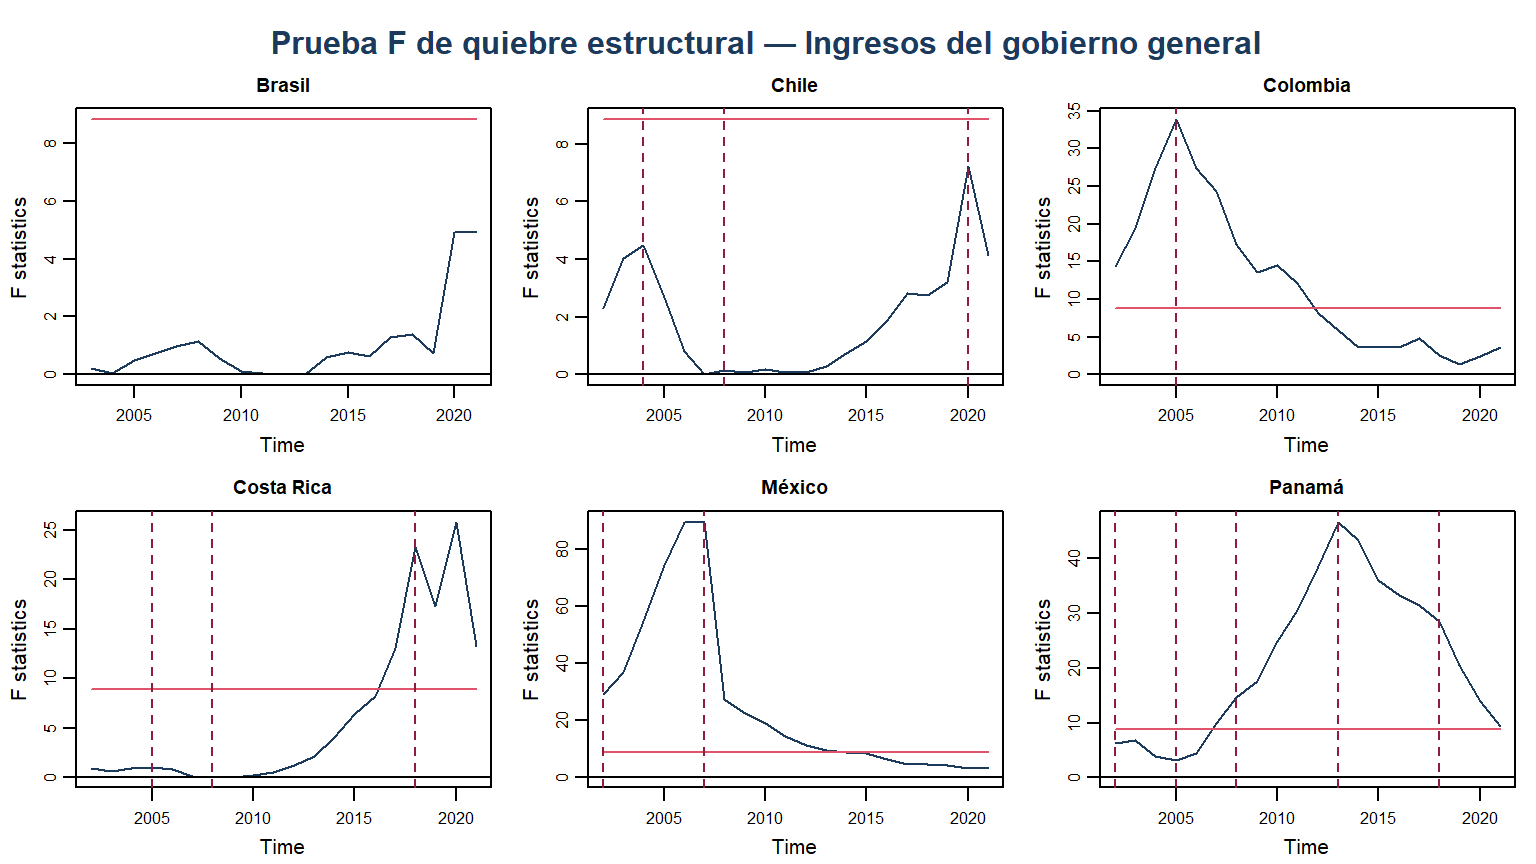
\includegraphics[width=\textwidth]{graficas/anexo_quiebres_ingresos_del_gobierno_general.png}
  \caption{Prueba F de quiebre estructural: ingresos del gobierno general. Línea
  horizontal: valor crítico al 5\,\%; líneas verticales: quiebres de Bai-Perron.}
  \label{fig:q-ingresos}
\end{figure}

\begin{figure}[htbp]
  \centering
  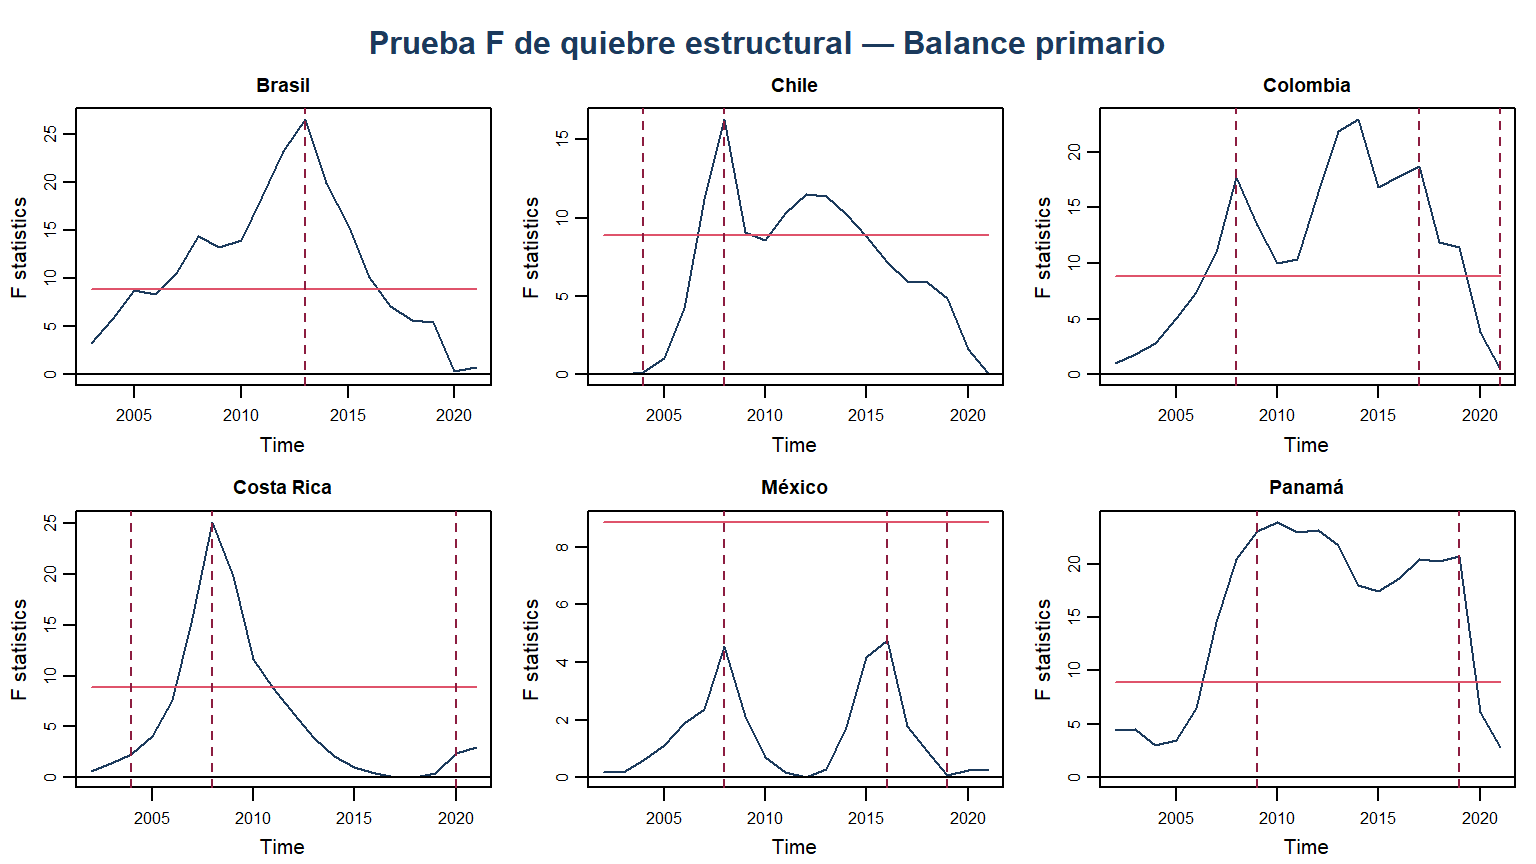
\includegraphics[width=\textwidth]{graficas/anexo_quiebres_balance_primario.png}
  \caption{Prueba F de quiebre estructural: balance primario.}
  \label{fig:q-balance}
\end{figure}

\begin{figure}[htbp]
  \centering
  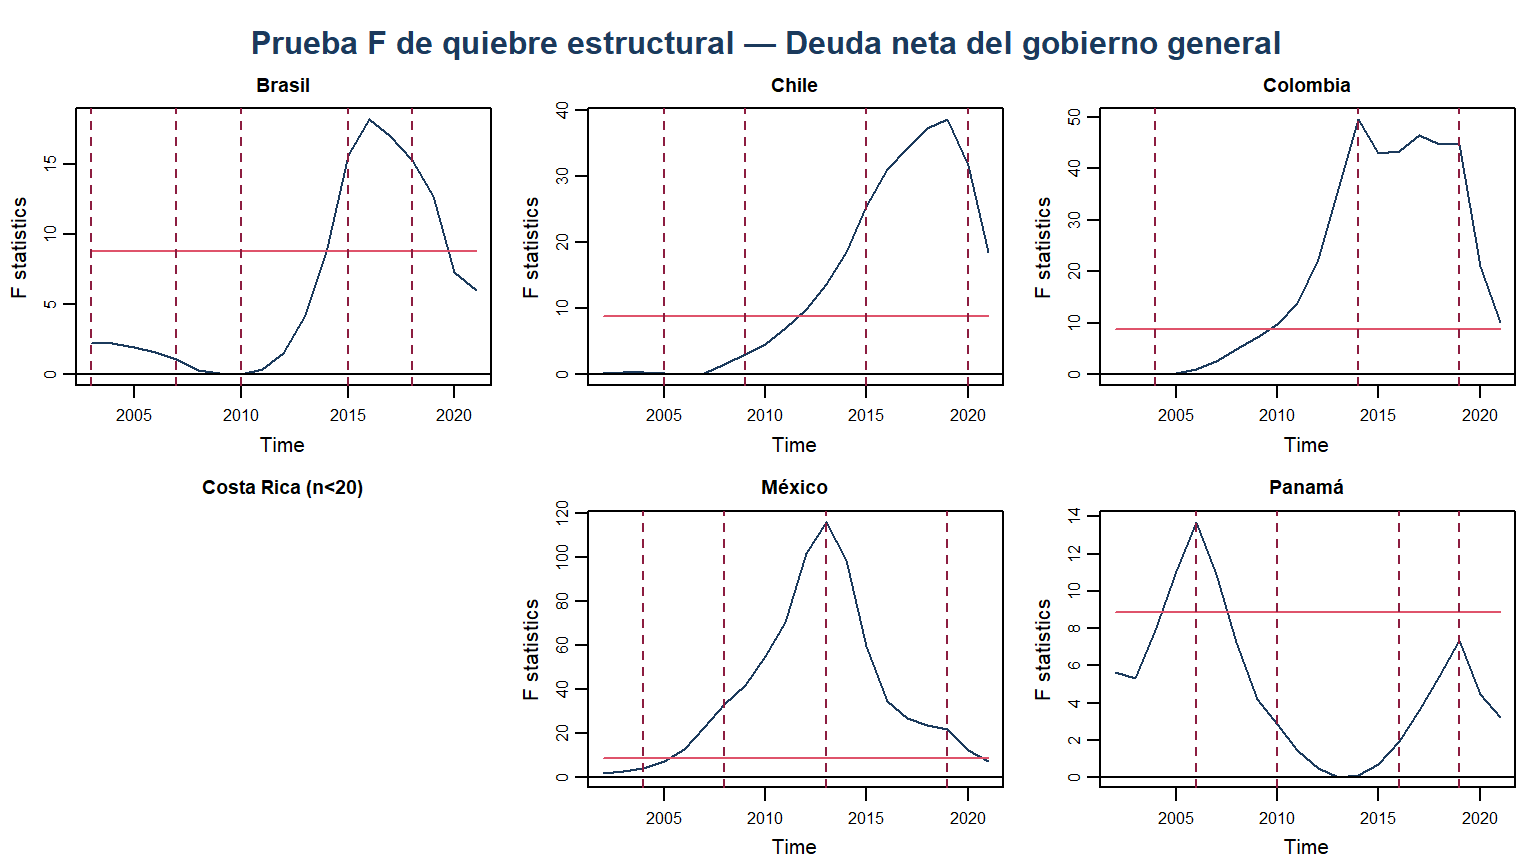
\includegraphics[width=\textwidth]{graficas/anexo_quiebres_deuda_neta_del_gobierno_general.png}
  \caption{Prueba F de quiebre estructural: deuda neta del gobierno general.}
  \label{fig:q-deuda}
\end{figure}

\begin{figure}[htbp]
  \centering
  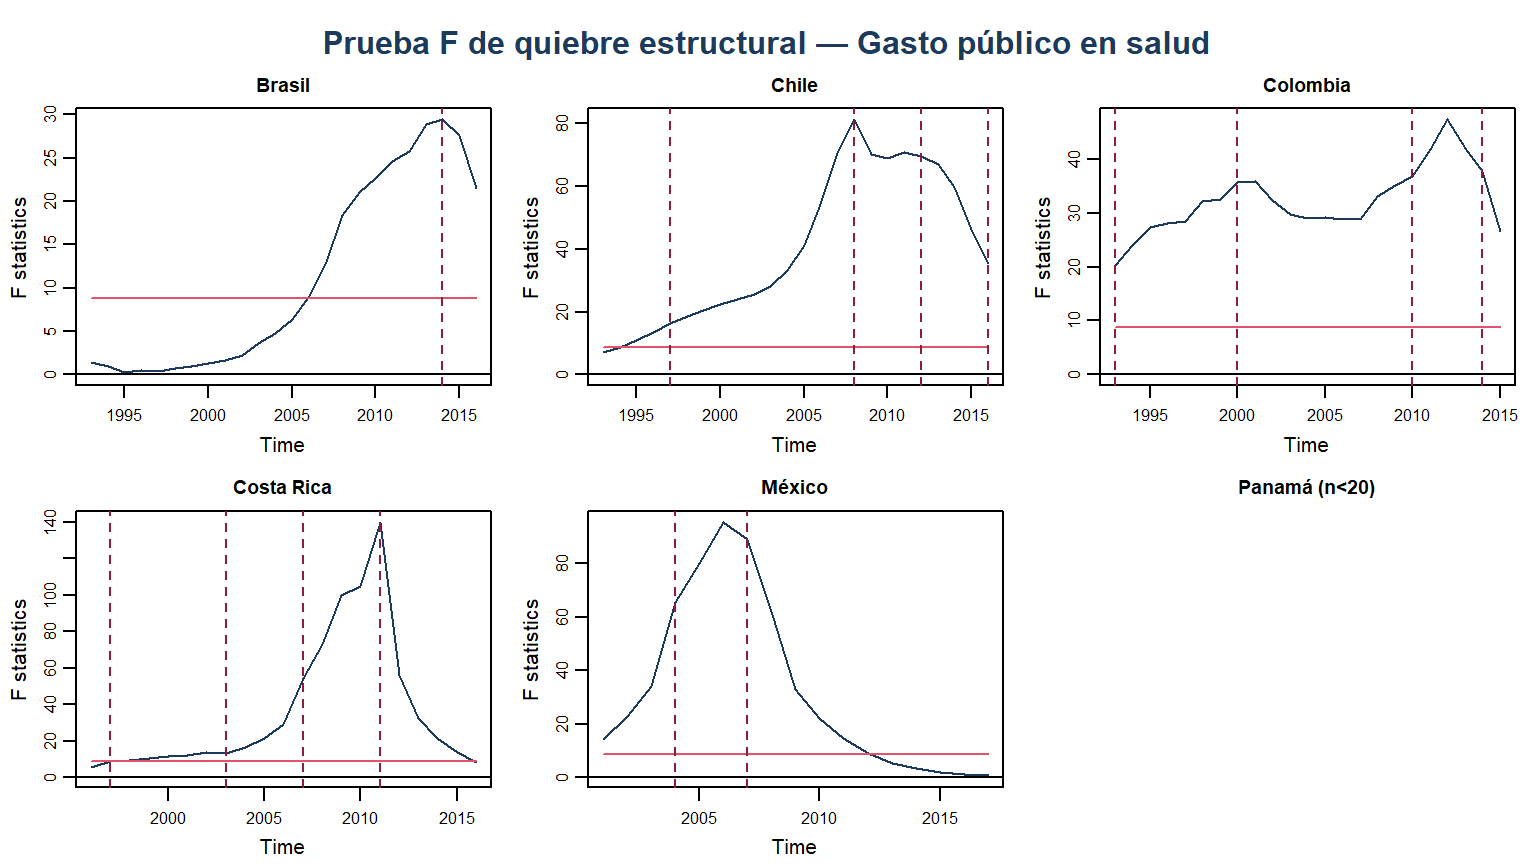
\includegraphics[width=\textwidth]{graficas/anexo_quiebres_gasto_publico_en_salud.png}
  \caption{Prueba F de quiebre estructural: gasto público en salud.}
  \label{fig:q-salud}
\end{figure}

\begin{figure}[htbp]
  \centering
  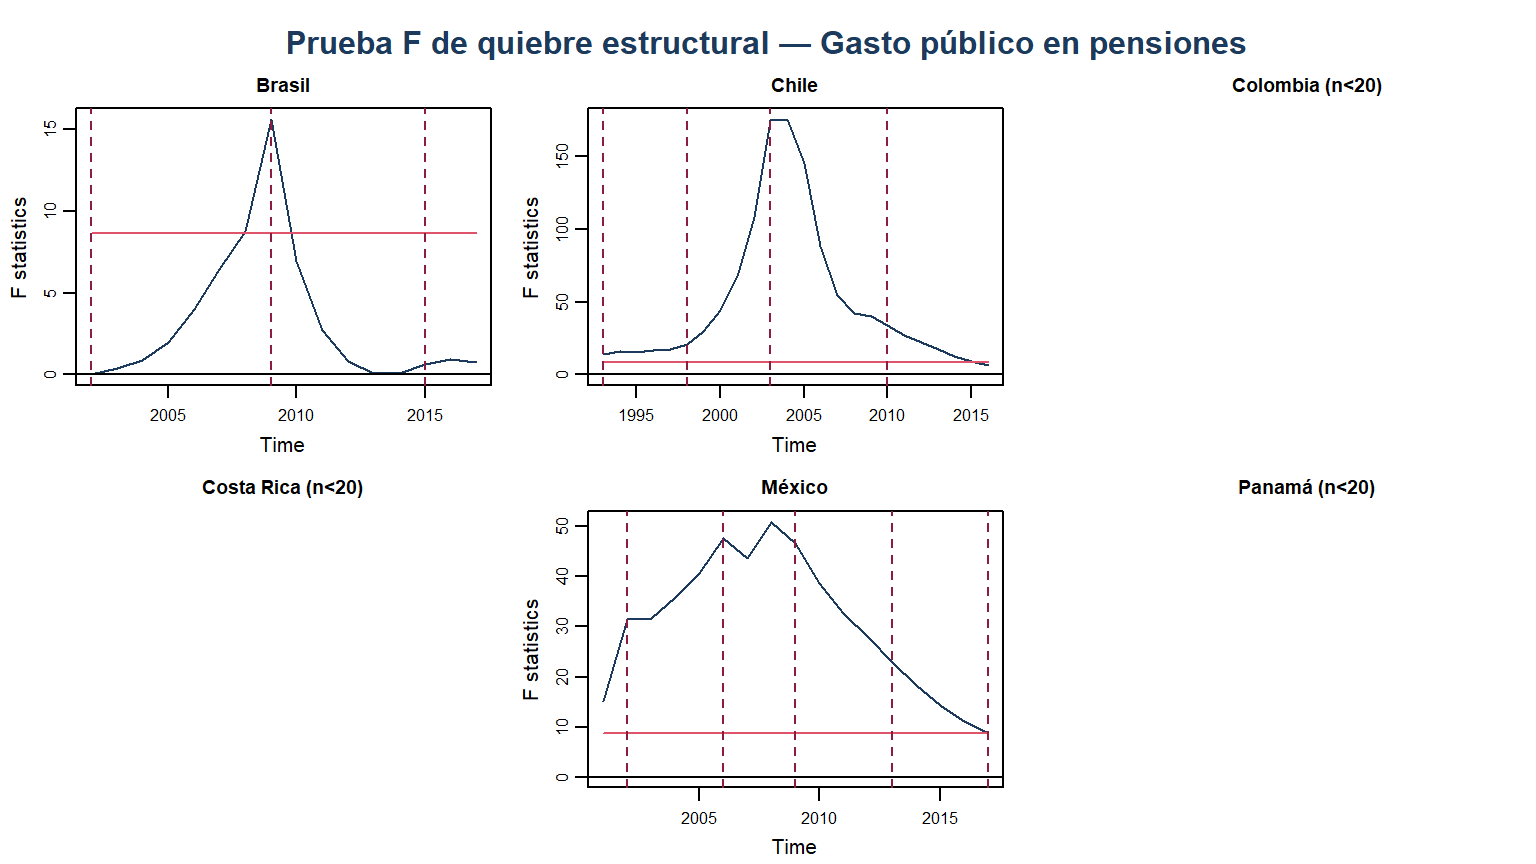
\includegraphics[width=\textwidth]{graficas/anexo_quiebres_gasto_publico_en_pensiones.png}
  \caption{Prueba F de quiebre estructural: gasto público en pensiones.}
  \label{fig:q-pensiones}
\end{figure}

\clearpage
\subsection{Diccionario de la base de datos}
\label{ap:diccionario}

Todo el análisis cuantitativo del documento se apoya en una base consolidada
única, \texttt{base\_analisis\_P4.csv}, que reúne las series demográficas y
fiscales de los seis países, las proyecciones propias corregidas y las dos series
del WEO incorporadas para el cálculo de la Sección~\ref{sec:espacio}. La
Tabla~\ref{tab:diccionario} reproduce su diccionario, incluida la advertencia de
uso actualizada, como respaldo de auditoría. La base de la versión intermedia
(\texttt{base\_analisis\_P3.csv}) se conserva sin modificación como registro de
procedencia.

\begin{table}[htbp]
  \centering
  \caption{Diccionario de \texttt{base\_analisis\_P4.csv}.}
  \label{tab:diccionario}
  \footnotesize
  \begin{tabular}{>{\raggedright\arraybackslash}p{4.3cm}>{\raggedright\arraybackslash}p{10.4cm}}
\toprule
Campo & Descripción \\
\midrule
\texttt{pais} & Nombre del país \\
\texttt{iso3} & Código ISO 3166-1 alfa-3 \\
\texttt{anio} & Año de referencia \\
\texttt{indicador} & Nombre del indicador \\
\texttt{codigo\_indicador} & Código de la serie en la fuente original \\
\texttt{tipo} & Observado | Estimación de la fuente | Proyección de la fuente | Proyección propia \\
\texttt{modelo} & Especificación empleada; vacío salvo en proyección propia \\
\texttt{valor} & Valor del indicador \\
\texttt{unidad} & Unidad de medida \\
\texttt{cobertura\_institucional} & Perímetro institucional del dato \\
\texttt{fuente} & Fuente primaria \\
\texttt{nota} & Advertencia de construcción o comparabilidad, cuando aplica \\
\midrule
\textbf{ADVERTENCIA DE USO} & \small Las proyecciones de gasto en salud y pensiones (tipo = 'Proyección propia') se re-estimaron en el Producto 4 (Opción 1: ventana de validación 2016-2019, anterior al choque de 2020). Tras la corrección 2 serie(s) siguen excediendo el rango histórico y conservan advertencia textual. Las series con MASE > 2 respecto del método ingenuo (Chile: ingresos del gobierno general; Costa Rica: ingresos del gobierno general; Brasil: balance primario; Chile: balance primario; Costa Rica: balance primario; Panamá: balance primario; Costa Rica: deuda neta del gobierno general; Colombia: gasto público en salud; México: gasto público en salud; Brasil: gasto público en pensiones) se conservan en la base marcadas como no informativas y no deben citarse como estimación puntual. El balance primario no se grafica: es estacionario y su extrapolación univariada no aporta información más allá de su media. Las series 'Crecimiento nominal del PIB' y 'Balance fiscal global' se incorporaron del WEO abril 2025 para el cálculo del diferencial (r - g) de la Sección 6. \\
\bottomrule
\end{tabular}

\end{table}


% =======================================================================
%  BIBLIOGRAFÍA
% =======================================================================
\newpage
\addcontentsline{toc}{section}{Referencias}

\begin{thebibliography}{99}

\bibitem[Aaron(1966)]{aaron1966} Aaron, H. (1966). The Social Insurance Paradox.
\textit{Canadian Journal of Economics and Political Science}, 32(3), 371--374.

\bibitem[Bai y Perron(2003)]{baiperron2003} Bai, J. y Perron, P. (2003).
Computation and Analysis of Multiple Structural Change Models.
\textit{Journal of Applied Econometrics}, 18(1), 1--22.

\bibitem[Banco Interamericano de Desarrollo(2026)]{bid2026} Banco Interamericano de
Desarrollo (2026). \textit{Spending Smarter}. Documento de trabajo financiado con
el apoyo de la Red de Investigación de América Latina y el Caribe del BID.
Copyright \copyright~2026 Inter-American Development Bank. Used by permission. The
opinions expressed in this publication are those of the authors and do not
necessarily reflect the views of the Inter-American Development Bank, its Board of
Directors, or the countries they represent.

\bibitem[CEPAL(2020)]{cepal2020} CEPAL (2020). \textit{El sistema de pensiones en
Costa Rica: institucionalidad, gasto público y sostenibilidad financiera}.
Elizondo, H., Pacheco, J.~F. y Pacheco, J.~C. Serie Macroeconomía del Desarrollo.
Santiago: Comisión Económica para América Latina y el Caribe.

\bibitem[DANE(2025)]{dane2025} Departamento Administrativo Nacional de Estadística
(2025). \textit{Estadísticas Vitales (EEVV): Nacimientos 2024, cifras preliminares}.
Boletín técnico, 26 de marzo de 2025. Bogotá: DANE.

\bibitem[Fernández-Villaverde(2026)]{fv2026} Fernández-Villaverde, J. (2026).
\textit{A Recent Population History of Latin America and the Caribbean}.
Presentación, 15 de septiembre de 2026. University of Pennsylvania, NBER y CEPR.
Material de presentación no publicado.

\bibitem[Holzmann y Hinz(2005)]{holzmann2005} Holzmann, R. y Hinz, R. (2005).
\textit{Old-Age Income Support in the 21st Century: An International Perspective
on Pension Systems and Reform}. Washington, DC: Banco Mundial.

\bibitem[INE(2025)]{ine2025} Instituto Nacional de Estadísticas de Chile (2025).
\textit{Boletín Demográfico Anual Provisional de Estadísticas Vitales 2024}.
Santiago: INE, 15 de mayo de 2025.

\bibitem[INEC Costa Rica(2025)]{ineccr2025} Instituto Nacional de Estadística y
Censos de Costa Rica (2025). \textit{Indicadores demográficos 2024}, Año 26. San
José: INEC, noviembre de 2025.

\bibitem[INEC Panamá(2025)]{inecpan2025} Instituto Nacional de Estadística y Censo,
Contraloría General de la República de Panamá (2025). \textit{Estadísticas Vitales,
Volumen II: Nacimientos vivos y defunciones fetales, año 2023}. Panamá: INEC, enero
de 2025.

\bibitem[INEGI(2024)]{inegi2024} Instituto Nacional de Estadística y Geografía
(2024). \textit{Encuesta Nacional de la Dinámica Demográfica (ENADID) 2023}.
Comunicado de prensa 305/24, 22 de mayo de 2024. Aguascalientes: INEGI.

\bibitem[Hyndman y Athanasopoulos(2021)]{hyndman2021} Hyndman, R.~J. y
Athanasopoulos, G. (2021). \textit{Forecasting: Principles and Practice},
3.\textsuperscript{a} ed. Melbourne: OTexts.

\bibitem[Krueger y Ludwig(2007)]{krueger2007} Krueger, D. y Ludwig, A. (2007). On
the Consequences of Demographic Change for Rates of Returns to Capital, and the
Distribution of Wealth and Welfare. \textit{Journal of Monetary Economics}, 54(1),
49--87.

\bibitem[World Bank(2025)]{wb2025} World Bank (2025). \textit{(In)Formalizing Jobs in Latin America
and the Caribbean}. Fietz, K., et al. Washington, DC: The World Bank.

\end{thebibliography}

\section*{Bases de datos}
\addcontentsline{toc}{section}{Bases de datos}

\begin{itemize}
  \item Naciones Unidas, División de Población. \textit{World Population
        Prospects 2024}, revisión mediana.
  \item Organización Mundial de la Salud. \textit{Global Health Expenditure
        Database} (GHED), clasificación SHA 2011.
  \item Organización Internacional del Trabajo. \textit{ILOSTAT}, indicadores de
        empleo informal.
  \item SEDLAC --- Socio-Economic Database for Latin America and the Caribbean
        (CEDLAS, Universidad Nacional de La Plata, y Banco Mundial).
  \item Fondo Monetario Internacional. \textit{World Economic Outlook}, abril de
        2025 (agregados fiscales del gobierno general; para la
        Sección~\ref{sec:espacio}, además, PIB nominal en moneda nacional y balance
        global del gobierno general).
  \item Registros vitales nacionales citados en la Sección~\ref{sec:insumo}:
        DANE (Colombia), INE (Chile), INEC (Costa Rica), INEGI (México), INEC y
        Contraloría General de la República (Panamá); véanse las entradas
        correspondientes en la bibliografía.
  \item CEPAL/FMI-GFS. Gasto público por función, cobertura de gobierno central.
\end{itemize}

\section*{Fuentes normativas}
\addcontentsline{toc}{section}{Fuentes normativas}

\begin{itemize}
  \item \textbf{México:} Constitución Política de los Estados Unidos Mexicanos
        (arts.\ 4.\textsuperscript{o}, 123 y 127); Ley del Seguro Social (1973 y
        1995); Ley del ISSSTE (2007); Ley de los Sistemas de Ahorro para el
        Retiro (1996).
  \item \textbf{Costa Rica:} Ley Constitutiva de la CCSS;
        Ley N.\textsuperscript{o}~2738 de 1961; Ley N.\textsuperscript{o}~7523 de
        1995; Ley de Protección al Trabajador N.\textsuperscript{o}~7983 de 2000;
        Ley Integral para la Persona Adulta Mayor N.\textsuperscript{o}~7935.
  \item \textbf{Panamá:} Ley 51 de 2005; Ley 86 de 2010; Ley 462 de 2025.
  \item \textbf{Colombia:} Constitución Política (art.\ 48); Ley 100 de 1993;
        Ley 797 de 2003; Ley 2381 de 2024 (vigencia general suspendida por el
        Auto A-841 de 2025 de la Corte Constitucional).
  \item \textbf{Brasil:} Constitución Federal de 1988 (arts.\ 40, 201, 202 y
        203); Emenda Constitucional 103/2019; Lei Orgânica da Assistência Social
        (LOAS, 1993); Leyes Complementarias 108 y 109 de 2001.
  \item \textbf{Chile:} Decreto Ley N.\textsuperscript{o}~3.500 de 1980;
        Ley N.\textsuperscript{o}~20.255 de 2008;
        Ley N.\textsuperscript{o}~21.419 de 2022;
        Ley N.\textsuperscript{o}~21.735 de 2025.
\end{itemize}

\end{document}
